\documentclass[a4paper,UTF8,fontset=windows]{ctexart}
\title{拓扑学H 作业解答}
\author{原生生物}
\date{}

\usepackage{amsmath,amssymb,enumerate,geometry,tikz}

\geometry{left = 2.0cm, right = 2.0cm, top = 2.0cm, bottom = 2.0cm}
\setlength{\parindent}{0pt}
\DeclareMathOperator{\diam}{diam}
\DeclareMathOperator{\Homeo}{Homeo}
\DeclareMathOperator{\Id}{Id}
\DeclareMathOperator{\lcm}{lcm}
\DeclareMathOperator{\supp}{supp}

\begin{document}
\maketitle
*对应王作勤老师《拓扑学H》课程作业,包含几乎全部Not Required部分。

\tableofcontents
\newpage
\section{第一周作业}
\subsection{}
\begin{enumerate}[(1)]
    \item
    a. $\Pi,\Sigma,\Psi,\Gamma,\Upsilon,\Omega,\pi,\gamma,\mu,\tau,\epsilon,+,\times,\cup,\sim,\to$
    
    b. $\heartsuit,\varphi,\alpha,\delta,\nabla,\propto$
    
    c. $\Phi,\phi,\theta,\beta$
    
    d. $\otimes$
    
    e. $\Theta$
    
    f. $\Xi$
    
    \item
    若其每个面均为六边形,设面数为$F$,由于每个面有六条边,两个面共用一条边,因此边数$E=\frac{6F}{2}=3F$,同理顶点数$V=\frac{6F}{3}=2F$,因此$V-E+F=0$,与多面体$V-E+F=2$矛盾。
    
    \item
    由$C$为简单闭曲线可知$f$在$(0,1)$上不为0,不妨设恒大于0。再令$[0,1]$外$f(x)=0$,使其在$\mathbb{R}$上连续。设$g(x)=f(x)-f(x+f(x))$,则$g$也在$\mathbb{R}$上连续。下证其在$(0,1)$上有零点。若否,其必然恒正或恒负:
    
    恒负:由于$f(x)<f(x+f(x))$,取$a_0\in(0,1),a_{n+1}=a_n+f(a_n)$,由于$f\ge0$知此数列单调,且不会超过$1+\max_{[0,1]}f(x)$,因此存在极限,设为$a$,由两边取极限知$a=a+f(a)$,因此$f(a)=0$,但$f(a_n)$单调增加且$f(a_0)>0$,矛盾。
    
    恒正:类似地,取$a_0\in(0,1),a_n=a_{n+1}+f(a_{n+1})$。由于$0+f(0)<a_n,a_n+f(a_n)>a_n$,必存在$0<a_{n+1}<a_n$满足递推,与上方类似得矛盾。
    
    由此,设$g(t)=0,t\in(0,1)$,可验证$(t,0),(t,f(t)),(t+f(t),0),(t+f(t),f(t))$即构成了满足要求的正方形。
    
    \item
    \begin{enumerate}[(a)]
    \item 计算端点处的值与0处、$\frac{1}{n}$处左右导数验证即可。
    \item \[\lim_{n\to\infty}F(u_n)=\lim_{n\to\infty}\int_0^\frac{1}{n}\frac{n^2\pi^2x^2}{4}\sin^2(n\pi x)\mathrm{d}x=\lim_{n\to\infty}\frac{1}{n}\int_0^1\frac{\pi^2x^2}{4}\sin^2(\pi x)\mathrm{d}x=\lim_{n\to\infty}\frac{C}{n}=0\]
    \item 若存在,由于$u(1)=1$且连续,$F(u)>0$,因此存在$m$使$F(u)>F(u_m)$,矛盾。
    \end{enumerate}
\end{enumerate}

\subsection{}
\begin{enumerate}[(1)]
    \item
    良定:若$p(x_1)=p(x_2),p(y_1)=p(y_2)$,则由于$\begin{cases}d(y_2,y_1)+d(y_1,x_1)+d(x_1,x_2)\ge d(y_2,x_2)\\d(y_1,y_2)+d(y_2,x_2)+d(x_2,x_1)\ge d(y_1,x_1)\end{cases}$,且$d(x_1,x_2)=d(y_1,y_2)=0$,由此$d(x_1,y_1)=d(x_2,y_2)$,从而此距离良好定义。
    
    正定:$\bar{d}(p(x),p(y))=d(x,y)\ge0,\bar{d}(p(x),p(y))=0\Leftrightarrow d(x,y)=0\Leftrightarrow p(x)=p(y)$
    
    对称:$\bar{d}(p(x),p(y))=d(x,y)=d(y,x)=\bar{d}(p(y),p(x))$
    
    三角不等式:$\bar{d}(p(x),p(y))+\bar{d}(p(y),p(z))=d(x,y)+d(y,z)\ge d(x,z)=\bar{d}(p(x),p(z))$
    
    \item
    \begin{enumerate}[(a)]
    \item
    $f(0)=f(d(x,x))=\tilde{d}(x,x)=0$,若$f$还有其他零点,考虑$\mathbb{R}$上$d(x,y)=|x-y|$即知矛盾。
    
    若有$f(\alpha)+f(\beta)<f(\alpha+\beta)$,在上方度量中考察$\tilde{d}(\alpha,0),\tilde{d}(0,-\beta),\tilde{d}(\alpha,-\beta)$即知矛盾。
    
    \item
    由$f^{-1}(\{0\})=\{0\}$可知正定,由$f(d(x,y))=f(d(y,x))$可知对称,故只须证明三角不等式。
    \begin{enumerate}[(i)]
    \item
    $\tilde{d}(x,y)+\tilde{d}(y,z)\ge f(d(x,y)+d(y,z))\ge f(d(x,z))=\tilde{d}(x,z)$
    
    \item
    只须证明其满足第一小问条件。以下利用凹函数性质:设$x<y$,则$t>y$时$f(t)\le l(t)$,其中$l$为连接$(x,f(x)),(y,f(y))$的直线(此性质可由斜率的不等式证明)。
    
    不减:若否,存在$x<y,f(y)>f(x)$,连线与$x$轴有交点,此后只能$f<0$,与值域矛盾。
    
    次可加:$(\alpha,f(\alpha)),(\beta,f(\beta)),0<\alpha<\beta$连线为$l(x)=\frac{f(\beta)-f(\alpha)}{\beta-\alpha}x+\frac{\beta f(\alpha)-\alpha f(\beta)}{\beta-\alpha}$,由此
    \[f(\alpha+\beta)\le l(\alpha+\beta)=f(\alpha)+f(\beta)-\frac{\beta f(\alpha)-\alpha f(\beta)}{\beta-\alpha}\le f(\alpha)+f(\beta)\]
    最后一步是由于连接$(0,0),(\alpha,f(\alpha))$可知$\frac{f(\alpha)}{\alpha}\ge\frac{f(\beta)}{\beta}$,于是$\beta f(\alpha)-\alpha f(\beta)\ge0$
    
    由此即得证。
    
    \item
    $f(d(x,y))+f(d(y,z))\ge c+c=2c\ge f(d(x,z))$
    \end{enumerate}
    \end{enumerate}
    
    \item
    \begin{enumerate}[(a)]
    \item
    设$x_n\to x_0$,对任意$a\in A$,$\begin{cases}d(x_0,a)+d(x_0,x_n)\ge d(x_n,a)\\d(x_n,a)+d(x_0,x_n)\ge d(x_0,a)\end{cases}$,由此
    \[\begin{cases}\inf_{a\in A}d(x_0,a)+d(x_0,x_n)\ge\inf_{a\in A}d(x_n,a)\\\inf_{a\in A}d(x_n,a)+d(x_0,x_n)\ge\inf_{a\in A}d(x_0,a)\end{cases}\]
    取极限后$\lim_{n\to\infty}d(x_0,x_n)=0$,因此有$\lim_{n\to\infty}d_A(x_n)=d_A(x_0)$。
    
    \item
    当:由条件,若$x\notin A$,则$d_A(x)=c>0$,由此$B_{\frac{c}{2}}(x)\subset A^c$,$A^c$为开集,$A$为闭集。
    
    仅当:由定义$A^c$开,由此$\forall x\notin A,\exists\varepsilon, B_\varepsilon(x)\subset A^c$,由此$d_A(x)\ge\varepsilon$,即得证。
    
    \item
    定义$f(x)=\frac{d_A(x)}{d_A(x)+d_B(x)}$,由(b)与两集合不交可知分母不可能为0,再由(a)知连续,可验证符合要求。 
    \end{enumerate}
    
    \item
    \begin{enumerate}[(a)]
    \item
    $\forall x\in X,\forall\varepsilon>0,\exists N,\forall n>N, d(f_n(x),f(x))<\varepsilon$
    
    \item
    设$x_m\to x_0$,对任意$\varepsilon$,取$N$使$\forall n>N, d(f_n(x),f(x))<\frac{1}{3}\varepsilon$,再取$M$使$m>M$时$d(f_n(x_m),f_n(x_0))<\frac{1}{3}\varepsilon$,则$m>M$时$d(f(x_m),f(x_0))\le d(f(x_m),f_n(x_m))+d(f(x_0),f_n(x_0))+d(f_n(x_m),f_n(x_0))<\varepsilon$,即证明连续。
    
    \item
    \begin{enumerate}[(i)]
    \item
    记$\phi(x)=\frac{x}{1+x}$,其满足(2)(b)(ii)条件,由此只需证明$d(f,g)=\sup_{x\in X}d_Y(f(x),g(x))$是度量(上界不存在定义为$\bar{d}$中1)。
    
    正定:由$d_Y$正定性知$d\ge0$,$d(f,g)=0\Leftrightarrow\forall x\in X,d_Y(f(x),g(x))=0\Leftrightarrow f=g$。
    
    对称:由$d_Y$对称知结论。
    
    三角不等式:由于$d_Y(f(x),g(x))+d_Y(g(x),h(x))\ge d_Y(f(x),h(x))$,取$\sup$后仍保持性质。
    
    \item
    由$\phi(x)$单调且在0处连续,
    \[\forall\delta,\exists N,\forall n>N, \bar{d}(f_n,f)<\delta\Leftrightarrow\forall\varepsilon,\exists N,\forall n>N, \sup_{x\in X}d_Y(f_n(x),f(x))<\varepsilon\]
    左侧即为度量空间意义下收敛,右侧即为一致收敛。
    \end{enumerate}
    \end{enumerate}
\end{enumerate}

\section{第二周作业}
\subsection{}
\begin{enumerate}[(1)]
    \item
    \begin{enumerate}[(a)]
    \item
    由于$\arctan{x}$在$\mathbb{R}$上单调增可知正定,由形式知对称,且
    \[|\arctan{x}-\arctan{y}|+|\arctan{y}-\arctan(z)|\ge|\arctan{x}-\arctan(z)|\]
    由此成立。
    
    \item
    由于$\arctan{x}$为单调连续函数,$\forall\varepsilon,\exists\delta,|x-y|<\delta\Rightarrow|\arctan{x}-\arctan{y}|<\varepsilon$。
    
    另一方面,由$\tan$连续类似可得$\forall\varepsilon,\exists\delta,|\arctan{x}-\arctan{y}|<\delta\Rightarrow|x-y|<\varepsilon$,由此考虑开集中每个点所属于的开球可知拓扑等价。
    
    由$d_0(x,y)<\pi$,$d(x,y)$无界可知不强等价。
    
    \item
    由于$\arctan{x}$导函数有界,在$\mathbb{R}$上一致连续,可知$f:(\mathbb{R},d)\to(\mathbb{R},d_0)$一致连续。
    
    $f:(\mathbb{R},d_0)\to(\mathbb{R},d)$并不一致连续。取$\varepsilon=1$,由于$\lim_{x\to\infty}\arctan{x}=\frac{\pi}{2}$,由柯西收敛定理可知$\forall\delta,\exists t,\forall x,y>t,|\arctan{x}-\arctan{y}|<\delta$,因此$|x-y|$可以任意大,矛盾。
    
    \item
    满足一致连续。设$d'_X$与$d_X$强等价,$d'_Y$与$d_Y$强等价,$f:(X,d_X)\to(Y,d_Y)$一致连续,下证$f:(X,d'_X)\to(Y,d'_Y)$一致连续。
    
    设$d_X\le C_1d'_X,d'_Y\le C_2d_Y$,$\forall\varepsilon>0,\exists\delta>0,d_X(x_1,x_2)<\delta\Rightarrow d_Y(f(x_1),f(x_2))<\frac{\varepsilon}{C_2}$,由此
    \[d'_X(x_1,x_2)<\frac{\delta}{C_1}\Rightarrow d_X(x_1,x_2)<\delta\Rightarrow d_Y(f(x_1),f(x_2))<\frac{\varepsilon}{C_2}\Rightarrow d'_Y(f(x_1),f(x_2))<\varepsilon\]
    
    由此得证。
    \end{enumerate}
    
    \item
    \begin{enumerate}[(a)]
    \item
    $W=U\times V,\varnothing=\varnothing\times\varnothing$均为开集。
    
    若$W_1,W_2$开集,对每个$(x,y)\in W_1\cap W_2$,设$x\in U_1,y\in V_1,U_1\times V_1\subset W_1;x\in U_2,y\in V_2,U_2\times V_2\subset W_2$,则考虑邻域$U_1\cap U_2\times V_1\cap V_2$即知$W_1\cap W_2$为开集。
    
    若有一族开集,对并中每个$(x,y)$直接取其原来所在某个中邻域即知其并为开集。
    
    由此即验证了其为拓扑空间。
    
    \item
    \begin{enumerate}[(i)]
    \item
    对某个$(x,y)\in U\times V$,设$B(x,a)\subset U,B(y,b)\subset V$,则考虑$B((x,y),\min(a,b))$。此球中的点$(s,t)$满足$d_X(x,s)+d_Y(y,t)\le\min(a,b)$,因此$s\in U,t\in V$,从而得证。
    
    \item
    当:由于$B(x,r)\times B(y,r)\subset W$,可验证$B((x,y),r)\subset W$,由此满足开集定义。
    
    仅当:对$(x,y)$,由开集知存在$r$使得$B((x,y),r)\subset W$,可验证$B(x,\frac{r}{2})\times B(y,\frac{r}{2})\subset W$,由此得证。
    \end{enumerate}
    
    \item
    与(b)中证明过程完全相同,可直接估算验证。
    \end{enumerate}
    
    \item
    \begin{enumerate}[(a)]
    \item
    O1: 由定义空集为开集,由邻域非空与N2可知$X$为开集。
    
    O2: 由N3可知两开集的交仍为开集。
    
    O3: 由N2可知开集的任意并仍为开集。
    
    \item
    
    N1: 由定义知成立。
    
    N2: 由$U\subset N,N\subset M$可知$U\subset M$,因此成立。
    
    N3: 设$x\in U_1,U_1\subset N_1;x\in U_2,U_2\subset N_2$,由于$U_1,U_2$为开集,其交集亦为开集,且包含于$N_1\subset N_2$,由此得证。
    
    N4: 取$M$为$U$,由定义可验证成立。
    
    \item
    如果不存在N4,不同邻域结构可能对应相同的拓扑:
    
    设$X=\{1,2,3\}$,1邻域为$\{1\},\{1,2\},\{1,3\},X$,2邻域为$\{1,2\},X$,3邻域只有$X$或为$X$与$\{2,3\}$,对应的拓扑中开集均为$\varnothing,\{1\},\{1,2\},X$。
    
    \item
    拓扑$\to$邻域$\to$拓扑:若$U$为开集,根据诱导邻域定义,其必在其中每个点的邻域中,因此为邻域诱导的开集。若$U$为邻域诱导的开集,根据邻域定义,对每个点$x\in U$,存在原本开集$U_x$,$x\in U_x,U_x\subset U$,因此$U=\bigcup_xU_x$,由$U_x$为原本开集知$U$为原本开集。
    
    邻域$\to$拓扑$\to$邻域:若$N$原本为$x$邻域,考虑所有以$N$为邻域的点组成的集合$A$,利用N4考虑每个点对应的$M$可知$A$中任何点都以$A$为邻域,从而$A$为包含$x$的开集,$N$为诱导邻域系统中$x$的邻域。若$N$为诱导邻域系统中$x$的邻域,由于其中有包含$x$开集,而开集为其中任何点邻域,由N2知$N$原本即为$x$邻域。
    
    由以上两点知(a)(b)的过程可逆,从而两系统等价。
    \end{enumerate}
    
    \item
    \begin{enumerate}[(a)]
    \item
    \begin{enumerate}[(i)]
    \item
    空集由定义为开集,$\forall a,N_{a,1}\subset\mathbb{Z}$,故为开集。
    
    对两个开集的交,设$a\in U_1\cap U_2,N_{a,b_1}\subset U_1,N_{a,b_2}\subset U_2$,可验证$N_{a,b_1b_2}\subset U_1\cap U_2$,从而得证。
    
    由定义可知任意开集的并仍为开集,由此其为拓扑。
    
    \item
    $\forall x\in N_{a,b},N_{x,b}=N_{a,b}$,从而其为开集。
    
    \item
    由开集的并为开集可知$\bigcup_{i=1}^{n-1}N_{b+i,b}$为开集,可验证其补集即为$N_{a,b}$,故为闭集。
    
    \item
    由于正负1外的任何整数至少有一个素因子,原式成立。
    
    \item
    若此集合有限,根据(iii)可知(iv)中定义的集合为闭集的有限并,因此为闭集,从而其补集$\{-1,1\}$为开集,这与开集定义矛盾,从而素数有无穷多个。
    \end{enumerate}
    
    \item
    \begin{enumerate}[(i)]
    \item
    由定义知正定、对称。当$a,b,c$有相等时三角不等式成立,否则设$\tau(a-b)=x,\tau(b-c)=y$,则$\forall t<\min(x,y),t|a-b,t|b-c\Rightarrow t|b-c$,因此$\tau(b-c)\ge\min(x,y)$,从而$d(a,c)\le\max(d(a,b),d(b,c))$,自然小于其和。
    
    \item
    每个$B(a,r)$都代表着与$a$的差距能整除某个$\lcm(1,2,\dots,k),k\in N^*$的整数集合。
    
    \item
    对度量诱导拓扑下开集$U$,其若非空,由(ii)知必有$N_{a,t}\subset U,t=\lcm(1,2,\dots,k)$,由此为拓扑下开集。
    
    对拓扑下非空开集$U$,$\forall a,\exists N_{a,b}\subset U$,取$t=\lcm(1,2,\dots,b)$则$N_{a,t}\subset U$,由此$B(a,2^{-b})\in U$,从而为度量诱导拓扑下开集。
    
    因此此拓扑即为度量诱导的拓扑。
    \end{enumerate}
    \end{enumerate}
\end{enumerate}

\subsection{}
\begin{enumerate}[(1)]
    \item
    \begin{enumerate}[(a)]
    \item
    空集与全集为开集。开集的交取$\varepsilon_1,\varepsilon_2$中较小者可知仍为开集,开集的并由定义仍开,由此其为拓扑。
    
    \item
    开集对任意$x$直接取$\varepsilon=b-x$即可。其补集中,若$x<a$,取$\varepsilon=a-x$,否则取$\varepsilon=1$,即可知补集为开集,因此其为闭集。
    
    \item
    对$\mathbb{R}$上任何寻常开集,由于其对每个$x$包含$(x-\varepsilon,x+\varepsilon)$,必然包含$[x,x+\varepsilon)$,由此为此拓扑开集。而$[0,1)$不为寻常拓扑中开集,因此严格强。
    
    \item
    考虑$[x,x+\varepsilon)$这样的开集即知需要通常意义收敛且只有至多有限多项在$x$左侧。
    
    \item
    当:由于连续必然序列连续,而由(d)可得此拓扑下收敛即为右极限,从而知右连续。
    
    仅当:设$f(x)$包含于某通常开集$U$,由右连续,$\forall\varepsilon,\exists\delta,t\in[x,x+\delta)$时$|f(t)-f(x)|<\varepsilon$,从而可知存在$x$的邻域使其像包含于$U$,因此$U$的原像是开集,即证明了连续。
    
    \item
    定义$U\subset\mathbb{R}$为开集当且仅当$U=\varnothing,\mathbb{R}$或$\exists a\in\mathbb{R},U=(-\infty,a)$。对并集$\bigcup_iU_i$取$a'=\sup_ia_i$可知其为开集,从而可验证其为拓扑。
    
    当:此拓扑下$x_n$收敛于$x$即为$\forall\varepsilon,\exists N,\forall n>N,x_n<x+\varepsilon$,从而由连续必然序列连续可推出上半连续。
    
    仅当:与(e)中仅当类似验证,利用上半连续定义可得连续。
    \end{enumerate}
    
    \item
    \begin{enumerate}[(a)]
    \item
    对$Y$中任何闭集,其在$f|_A$与$f|_B$下原像$U,V$均为子空间拓扑意义下闭集,由$A,B$为闭集与闭集交集为闭集可知$U,V$均为闭集。由此其在$f$下原像为两原像并集$U\cup V$,两闭集的并仍为闭集,从而$f$任意闭集的原像是闭集,因此连续。
    
    \item
    $X=[0,1],Y=\mathbb{R},A_n=\begin{cases}\{0\}&n=1\\\big[\frac{1}{n},\frac{1}{n-1}\big]&n>1\end{cases},f(x)=\begin{cases}0&x=0\\\frac{1}{x}&x>0\end{cases}$即为反例。
    
    \item
    将$(a)$中的闭集替换为开集,通过开集的并集仍为开集即得证。
    \end{enumerate}
    
    \item
    \begin{enumerate}[(a)]
    \item
    对球上任何点$(x_1,\dots,x_{n+1})$,将其与$N$点连线得到$(tx_1,\dots,tx_n,1-t+tx_{n+1}),t\in\mathbb{R}$,与$\mathbb{R}^n$交点为$(\frac{x_1}{1-x_{n+1}},\dots,\frac{x_n}{1-x_{n+1}},0)$,由此球极投影$(x_1,\dots,x_{n+1})\to(\frac{x_1}{1-x_{n+1}},\dots,\frac{x_n}{1-x_{n+1}})$即为所求同胚。
    
    \item
    不妨设$n>m$,由于$\mathbb{R}^m$可看作$\mathbb{R}^n$子集,由区域不变性定理可知若存在同胚$f:\mathbb{R}^n\to\mathbb{R}^m\subset\mathbb{R}^n$,由于其为连续双射,必为开映射。但开集$\mathbb{R}^n$的像$\mathbb{R}^m$不为开集,矛盾。
    
    \item
    由于$f$为连续双射,限制后的$f$仍为连续双射。由于$X\backslash A$中开集为原开集与$X\backslash A$的交,其像集为原本像集与$Y\backslash f(A)$之交。由原本为开映射可知限制后的$f$仍为开映射,结合连续双射知同胚。
    
    \item
    $\Id$映射即为单位元,由同胚的复合与逆也是同胚、映射复合具有结合律可知构成群。
    
    若有同胚$\varphi:X\to Y$,则可验证$\varphi^*:\Homeo(X)\to\Homeo(Y),\varphi^*(f)=\varphi\circ f\circ\varphi^{-1}$即为同构。
    \end{enumerate}
    
    \item
    *此题将几乎处处相等的函数视为同一函数
    \begin{enumerate}[(a)]
    \item
    由几乎处处相等视为同一函数可知正定,由定义可知对称,分类讨论验证$\min(|f(x)-g(x)|,1)+\min(|g(x)-h(x)|,1)\ge\min(|f(x)-h(x)|,1)$,从而满足三角不等式。因此其为度量。
    
    \item
    当:由于度量意义下收敛,$\forall\varepsilon>0,\exists N,\forall n>N,d(f_n,f)<\varepsilon$,从而$\forall\sigma>0$,$m\{|f_n(x)-f(x)|\ge\sigma\}<\frac{\varepsilon}{\sigma}$。由此,$\forall\varepsilon,\delta>0$取$N$使$n>N$时$d(f_n,f)<\delta\varepsilon$,即有$m\{|f_n(x)-f(x)|\ge\delta\}<\varepsilon$,故依测度收敛。
    
    仅当:由依测度收敛定义,$\forall\varepsilon,\sigma>0,\exists N,\forall n>N,m\{|f_n(x)-f(x)|\ge\delta\}<\varepsilon$,设$|f(x)|\le M$,则$d(f_n,f)<\delta+M\varepsilon$,变化$\delta,\varepsilon$即可知度量意义下收敛。
    
    \item
    构造$f(x)=0$,$f_n(x)=1$当且仅当$\exists 0<t<\frac{1}{n+1},x=\{\sum_{k=1}^{n}\frac{1}{k}+t\}$(大括号代表小数部分),否则为0。
    
    由于$f_n$仅在长度为$\frac{1}{n+1}$的区间上为1,其依测度收敛于$f$,但由调和级数发散可知除1外每个点会无穷次取到1,因此不满足几乎处处收敛。
    
    此例子结合提示过程即可得到完整证明。
    \end{enumerate}
\end{enumerate}

\section{第三周作业}
\subsection{}
\begin{enumerate}[(1)]
    \item
    \begin{enumerate}[(a)]
    \item
    $\mathcal{N}(x)=\{N|\exists B\in\mathcal{B}(x),B\subset N\}$
    
    \item
    设集族$\mathcal{S}(x)\subset \mathcal{P}(X)$满足$\forall S\in\mathcal{S}(x), x\in S$,记$\mathcal{B}(x)=\{B|\exists S_1,\dots,S_m\in S,B=S_1\cap\dots\cap S_m\}$,则$\mathcal{B}(x)$成为邻域基,$\mathcal{S}(x)$成为邻域子基。
    
    \item
    记$f:Y\to X,f(y)=x$,则$f$在$y$连续
    
    $\Longleftrightarrow\forall B\in\mathcal{B}(x)$,$f^{-1}(B)$为$y$邻域
    
    $\Longleftrightarrow\forall S\in\mathcal{S}(x)$,$f^{-1}(S)$为$y$邻域
    
    根据邻域的定义与邻域基包含邻域子基,只需证明$\forall S\in\mathcal{S}(x)$,$f^{-1}(S)$为$y$邻域$\Longrightarrow f$在$y$连续。
    
    由于邻域的有限交仍为邻域,$f^{-1}(S_1)\cap f^{-1}(S_2)=f^{-1}(S_1\cap S_2)$可知$\forall B\in\mathcal{B}(x)$,$f^{-1}(B)$为$y$邻域。而对任何$x$的邻域$N$,设$B_0\subset N$,则$f^{-1}(B_0)\subset f^{-1}(N)$,从而$x$的任何邻域原像为$y$邻域,命题得证。
    \end{enumerate}
    
    \item
    \begin{enumerate}[(a)]
    \item
    由于子基(基)生成的拓扑是包含子基(基)的最小拓扑,只需证明乘积拓扑的子基都是一致拓扑下的开集,一致拓扑的基都是箱拓扑下的开集。
    
    乘积拓扑的一组子基中元素$S$为第$i$个分量是通常$\mathbb{R}$上开集$U$,其余分量为$\mathbb{R}$的笛卡尔积。$\forall x\in S,\exists r, B(x_i,r)\subset U$,由此一致拓扑下$B(x,\min(r,\frac{1}{2}))\subset S$,从而为开集。
    
    一致拓扑的基为$B(x,r),r>0$,可验证其为$\begin{cases}(x_1-r,x_1+r)\times(x_2-r,x_2+r)\times\cdots&r\le1\\X&r>1\end{cases}$,每个分量均为开集,由此是箱拓扑下开集。
    
    \item
    由例1.80可知逐点收敛拓扑的一个子基为全体某分量是$(x_i-\varepsilon,x_i+\varepsilon),x_i\in\mathbb{R},\varepsilon>0$,其余为$\mathbb{R}$的集合。由于$(x_i-\varepsilon,x_i+\varepsilon),x_i\in\mathbb{R},\varepsilon>0$是$\mathbb{R}$上通常拓扑的一组基,此子基亦为乘积拓扑的一组子基。由此两拓扑子基相同,故拓扑相同。
    
    \item
    对乘积拓扑,考虑的一组子基(一个分量为开集,其余分量为$\mathbb{R}$),由于每个分量为连续映射,$\mathbb{R}$的原像为$\mathbb{R}$,开集分量的原像为开集,因此子基的原像为开集,由此乘积拓扑下连续。
    
    对箱拓扑,考虑的一组基(每个分量均为开集),由于每个分量为连续映射,基的原像的每个分量仍为开集,由此基的原像为开集,因此箱拓扑下仍连续。
    \end{enumerate}
    
    \item
    \begin{enumerate}[(a)]
    \item
    当:由命题1.83知只需说明$f^{-1}(f_\beta^{-1}(V_\beta))$为开集,其中$V_\beta\subset Y_\beta$为开集,而其即为$(f_\beta\circ f)^{-1}(V_\beta)$,由此为开集。
    
    仅当:由连续映射复合连续知结果。
    
    唯一:若还有某拓扑满足,考虑其与$X$的诱导拓扑之间作恒等映射。利用泛性质可知此映射与逆均连续,由此两拓扑相同。
    
    \item
    当:由条件,对$Z$的任何开集$U$,$f_\alpha^{-1}(f^{-1}(U))$为开集,由此$f^{-1}(U)$在每个$f_\alpha$下的原像开,由余诱导拓扑的显示表达可知其为开集,从而得证。
    
    仅当:由连续映射复合连续知结果。
    
    唯一:若还有某拓扑满足,考虑其与$Y$的诱导拓扑之间作恒等映射。利用泛性质可知此映射与逆均连续,由此两拓扑相同。
    \end{enumerate}
    
    \item
    构造恒等映射$\Id:\prod_{\alpha}X_\alpha\to\prod_{\beta}\prod_{\alpha\in\Lambda_\beta}X_\alpha$。利用乘积映射泛性质,$f$为连续映射当且仅当其每个$\pi_\beta\circ\Id:\prod_{\alpha}X_\alpha\to\prod_{\alpha\in\Lambda_\beta}X_\alpha$为连续映射,再次使用即得当且仅当$\pi_\alpha\circ\pi_\beta\circ\Id:\prod_{\alpha}X_\alpha\to X_\alpha$为连续映射,而此映射即为$\prod_{\alpha}X_\alpha$上投影映射,由此连续。
    
    另一方面,恒等映射$\Id:\prod_{\beta}\prod_{\alpha\in\Lambda_\beta}X_\alpha\to\prod_{\alpha}X_\alpha$连续当且仅当$\pi_\alpha\circ\Id:\prod_{\beta}\prod_{\alpha\in\Lambda_\beta}X_\alpha\to X_\alpha$连续,而此映射可拆为$\prod_{\beta}\prod_{\alpha\in\Lambda_\beta}X_\alpha\to\prod_{\alpha\in\Lambda_\beta}X_\alpha$与$\prod_{\alpha\in\Lambda_\beta}X_\alpha\to X_\alpha$两个投影映射的复合,因此连续。
    
    由以上两方面可得两拓扑相同。
\end{enumerate}

\subsection{}
\begin{enumerate}[(1)]
    \item
    构造映射$\phi:\mathbb{R}\mathbb{P}^2\to\mathbb{R}^4$,$\varphi(x:y:z)=\frac{1}{x^2+y^2+z^2}(y^2-x^2,xy,xz,yz)$。
    
    良定性:由于分母不可能为0且分式上下每项都为两次,对等价的$(x:y:z)$映射到同一点。
    
    连续:记商映射$g:S^2\to\mathbb{R}\mathbb{P}^2$,$g(x,y,z)=(x:y:z)$,可验证$f=\varphi\circ g$。由于每个分量均为初等函数,$f$连续,从而由商映射泛性质可知$\varphi$连续。
    
    满射:同样由$f=\varphi\circ g$可知满射。
    
    单射:当且仅当$x,y,z$均不为0时,后三个分量均不为0,从而考虑倒数之比可还原出$(x:y:z)$。再分类讨论一个分量为0与两个分量为0的情况可知为单射。
    
    综合以上,利用闭映射引理(紧集到豪斯多夫空间的连续双射为同胚)可知$\varphi$为同胚,从而得证。
    
    \item
    \begin{enumerate}[(a)]
    \item
    设$x=(x_1,\dots,x_{n+1})\in S^n,t\in[0,1]$,定义$\varphi:C(S^n)\to B^{n+1}$,$\varphi(x,t)=tx$,可验证符合要求。
    
    \item
    仍沿用(a)中记号,定义$\varphi:S(S^n)\to S^{n+1}$,$\varphi(x,t)=(2\sqrt{t-t^2}x,2t-1)$,由于$2\sqrt{t-t^2}=\sqrt{1^2-(2t-1)^2}$,可验证符合要求。
    
    \item
    设$x=(x_1,\dots,x_n)\in B^n$,定义$\varphi:B^n/S^{n-1}\to S^n$,$\varphi(x)=\left(2\dfrac{\sqrt{||x||-||x||^2}}{||x||}x,2||x||-1\right)$,类似(b)可验证符合要求。
    \end{enumerate}
    
    \item
    \begin{enumerate}[(a)]
    \item
    开映射:当$V\subset Y$为开集时,由连续知$p^{-1}(V)$为开集。当$p^{-1}(V)$为开集时,由于$p(p^{-1}(V))=V$与开映射可知$V$为开集,从而得证。
    
    闭映射:仿照开映射的证明,取补集即可。
    
    \item
    设$X=\{1,2,3\}$,开集为$\varnothing,\{1\},\{1,2\},X$。令$Y=\{1,2\}$,$p(1)=p(3)=1,p(2)=2$。可验证$p$诱导的商拓扑只有$\varnothing,Y$为开集,取开集$\{1\}$与闭集$\{3\}$可知$p$非开非闭。
    
    \item
    \begin{enumerate}[(i)]
    \item
    满射:计算可知$f$的结果为矩阵的最后一列构成的向量,取包含这个向量的一组$\mathbb{R}^n$的标准正交基组成矩阵(若此时行列式为$-1$将第一列取为相反数即可),即为$S^{n-1}$中元素的原像。
    
    连续:$f$可看作$\mathbb{R}^{n^2}$到$\mathbb{R}^n$的投影映射,由此连续。
    
    开:由于$x$在$\mathbb{R}^{n^2}$中的邻域在投影后仍然为邻域,此映射为开映射。
    
    \item
    由(i)知$f$的纤维为所有最后一列相同的$SO(n)$中矩阵,而$A\begin{pmatrix}B&0\\0&1\end{pmatrix}$不改变最后一列,由此所在轨道必然包含于纤维。
    
    对于$A,A'$满足$Ae_1=A'e_1$,可知$A'^TAe_1=e_1$,即$A'^TA=\begin{pmatrix}B&0\\c&1\end{pmatrix}$,由于正交阵的逆与乘积仍正交,可知$c=1$,从而$A'^TA=\begin{pmatrix}B&0\\0&1\end{pmatrix}$,利用正交基可验证$B\in SO(n-1)$,而$A'(A'^TA)=A$,因此$A'$与$A$位于同一轨道。
    
    综合以上可知群作用的轨道与$f$的纤维相同。
    
    \item
    利用(ii),构造映射$p:SO(n)\to SO(n)/SO(n-1)$,$p(A)=[A]$,$[A]$代表所有满足$A'=A\begin{pmatrix}B&0\\0&1\end{pmatrix},B\in SO(n-1)$的矩阵构成的等价类。利用(ii)可知$f^*(p(A))=f(A)$良好定义,从而由上方证明可验证$f^*$即为同构。
    \end{enumerate}
    \end{enumerate}
    
    \item
    \begin{enumerate}[(a)]
    \item
    由群作用定义,$\forall g,\tau_g(x)$为连续映射,由于$U$为开集,在此映射下的原像$(\tau_g)^{-1}U$为开集。由于$\tau_{g^{-1}}\circ\tau_g=\tau_g\circ\tau_{g^{-1}}=\Id$,$\tau_g$为双射且其逆即为$\tau_{g^{-1}}$。由此,$\tau_{g^{-1}}(U)$为开集。由于$g^{-1}$可取遍群中元素,$\tau_g(U)$为开集。当
    
    利用商映射的性质,欲证明$p(U)$为开集,只需说明$p^{-1}(p(U))$为开集,由轨道定义,此即为$\bigcup_{g\in G}\tau_g(U)$,由开集的并为开集可知其开。
    
    \item
    连续:由商映射与群作用定义可知$p,\tau_g$连续,由此其复合连续。
    
    双射:(a)中证明了$\tau_g$为双射,从而只需要证明$U\to p(U)$为双射。满射由定义成立。若其不为单射,也即存在不同元素$u_1,u_2$在同一轨道中,设$g\cdot u_1=u_2$,则$u_2\in g\cdot U\cap U$,矛盾。
    
    逆映射连续:由$\tau_g$与$\tau_{g^{-1}}$互逆已说明了此部分连续,故只需说明$p:U\to p(U)$为开映射。对$U$中任何开集$U_0$,与(a)完全相同方法可说明$p(U_0)$开,由此得证。
    \end{enumerate}
\end{enumerate}

\section{第四周作业}
\subsection{}
\begin{enumerate}[(1)]
    \item
    当:由于序列连续,对$f(x_0)$的任何邻域$N$,若$f^{-1}(N)$不是$x_0$的邻域,考虑$x_0$的一组可数邻域基$U_n$,并每次将前$k$个取交得到一组越来越小的可数邻域基$U_n'$。由于$f^{-1}(N)$不为$x_0$邻域,其不包含邻域基中的任何一个,故可在每个$U_i'$中取出一个$x_i$使得其不在$f^{-1}(N)$中,从而得到了一个$f(x_i)\notin N,x_i\to x_0$的序列,与序列连续矛盾。
    
    仅当:之前讲义已证明连续必然序列连续。
    
    \item
    \begin{enumerate}[(a)]
    \item
    左包含于右:若$x\in\overline{A\cup B}$,由定义$x$的任何开邻域与$A\cup B$有交。若$x$的任何开邻域与$A$有交,则$x\in\overline{A}$,已得证。若否,设$U$为$x$所有与$A$交为空的开邻域之并,仍为$x$的开邻域。对$x$的任何开邻域$V$,$V\cap U$与$A$交为空,且仍为开邻域,故$V\cap U\cap B\ne\varnothing$,因此$V\cap B\ne\varnothing$,从而$x\in\overline{B}$。
    
    右包含于左:见(b)。
    
    \item
    由定义,存在$\alpha$使得$x$任何开邻域与$A_\alpha$交非空,从而与$\bigcup_\alpha A_\alpha$交非空,因此得证。
    
    \item
    $A_n=(\frac{1}{n},1),\bigcup_{n=1}^\infty\overline{A_n}=(0,1],\overline{\bigcup_{n=1}^\infty A_n}=[0,1]$
    
    \item
    由(b),只需证右包含于左。若$x\in\overline{\bigcup_\alpha A_\alpha}$,设开邻域$U$与只与有限个$A_\alpha$(记为$A_1,\dots,A_n$)交非空,对$n$归纳证明$x$在至少其中之一的闭包中。
    
    $n=1$时,对$x$的任何开邻域$V$,$V\cap U$与$A_1$外的集合交为空,且仍为开邻域,故$V\cap U\cap A_1\ne\varnothing$,因此$V\cap A_1\ne\varnothing$,从而$x\in\overline{A_1}$。
    
    $n=k$时若成立,$n=k+1$时,若$x\in\overline{A_1}$则已得证,否则存在开邻域$V$与$A_1$交为空,则$V\cap U$为只与$A_2,\dots,A_{k+1}$交非空的开邻域,由归纳假设知结论成立。
    
    综合以上即得证。
    \end{enumerate}
    
    \item
    $f$连续当且仅当$\forall B\subset Y,f^{-1}(B^\circ)\subset f^{-1}(B)^\circ$。
    
    当:对任何开集$V\subset Y$,$f^{-1}(V^\circ)=f^{-1}(V)\subset f^{-1}(V)^\circ$,又由于$f^{-1}(V)^\circ\subset f^{-1}(V)$可知$f^{-1}(V)=f^{-1}(V)^\circ$,从而为开集,由此得证。
    
    仅当:由于$B^\circ$为开集,$f^{-1}(B^\circ)$为开集,且包含于$f^{-1}(B)$,由此包含于$f^{-1}(B)^\circ$。
    
    \item
    \begin{enumerate}[(a)]
    \item
    设$U,V\in\mathcal{N}(x)$,$U\preceq V\Leftrightarrow V\subset U$,则$U,V\preceq U\cap V$,由此可验证其为定向集。
    
    \item
    当:取定向集为(a)中构造,由定义$x$的任何邻域与$A$有交,对每个邻域,任取一交中的点构成网$(x_\alpha)$。对$x$的任意邻域$U$,取$\alpha=U$,则所有满足$\alpha\preceq\beta$的$V$有$V\subset U$,故$x_\beta\in U$,由此得证。
    
    仅当:若存在这样的网$(x_\alpha)$,由网收敛定义知$x$的任何邻域与$A$交均非空,由此得证。
    
    \item
    当:利用(b)可知,$\forall A\subset X$,若$x\in\overline{A}$,则$f(x)\in\overline{f(A)}$,从而$f(\overline{A})\subset\overline{f(A)}$,由此可知连续。
    
    仅当:由于$f$连续,$f(\overline{A})\subset\overline{f(A)}$,即$x\in\overline{A}\Rightarrow f(x)\in\overline{f(A)}$,由此利用(b)知结论。
    \end{enumerate}
\end{enumerate}

\subsection{}
\begin{enumerate}[(1)]
    \item
    闭映射:紧空间中闭集为紧集,其连续映射下像为紧集,Hausdorff空间中紧集为闭集,由此得证。
    
    逆紧映射:Hausdorff空间中紧集为闭集,其连续映射下原像为闭集,紧空间中闭集为紧集,由此得证。
    
    同胚:由2.1.20其为闭映射,从而其逆映射闭集的原像为闭集,连续,因此其为同胚。
    
    非Hausdorff:考虑紧Hausdorff拓扑到较弱拓扑恒等映射,由于包含关系可知其为连续映射,且其为双射,若满足Hausdorff则由2.1.21其为同胚,但由包含关系知逆映射不连续,矛盾。
    
    非紧:考虑较强拓扑到紧Hausdorff拓扑的恒等映射,由于包含关系可知其为连续映射,且其为双射,若满足紧则则由2.1.21其为同胚,但由包含关系知逆映射不连续,矛盾。
    
    \item
    \begin{enumerate}[(a)]
    \item
    紧:考虑开覆盖$\bigcup_{n=1}^\infty(-\infty,n)$可知不紧。
    
    序列紧:考虑序列$x_n=n$可知不序列紧。
    
    极限点紧:任何无穷子集,比其中某个元素大的点均为极限点,由此极限点紧。
    
    \item
    一切满足$\sup E=\max E<+\infty$的集合$E$。
    
    若$E$满足此条件,任何$E$的开覆盖必然包含$(-\infty,a),a>\sup E$,取出此开集即可覆盖$E$。
    
    若$E$无上界,类似(a)中构造即得矛盾;若$E$无法取到其上界,设$E$中的点列$e_i$在$\mathbb{R}$上通常意义下趋于上界,取开覆盖$\bigcup_{n=1}^\infty(-\infty,e_n)$则不存在有限子覆盖。
    
    \item
    紧集上的上半连续函数必可取到最大值。
    
    设$A$为$X$中紧集,其到$\mathbb{R}$的上半连续函数即为上半连续拓扑下的连续函数,由此紧集的像为上半连续拓扑中的紧集,由(b)知可取到最大值。
    \end{enumerate}
    
    \item
    \begin{enumerate}[(a)]
    \item
    对其闭子集$B$任何开覆盖$\bigcup_{n=1}^\infty U_n$,$B^c\cup\bigcup_{n=1}^\infty U_n$为空间的可数开覆盖,由此可取出有限个,再去除$B^c$即得子集的有限开覆盖。
    
    \item
    假设$S$无极限点,由导集为空可知其为闭集,若$S$为无穷集合,可从中取出可数子集$T$,仍为闭集。对$T$中每个点取邻域$U_n$使其中无$T$中其他点,与$T^c$构成空间的可数开覆盖,由此存在有限子覆盖,考虑$T$中点知$T$只能为有限集,矛盾。
    
    \item
    当:对任何可数开覆盖$\bigcup_{n=1}^\infty U_n$,记$V_k=\bigcup_{i=1}^kU_k$为开集,$F_k=V_k^c$,由于$F_k$为递减且交为空的闭集,其中必然存在空集,由此即得到有限子覆盖。
    
    仅当:若$\bigcap_{n=1}^\infty F_n=\varnothing$,$\bigcup_{n=1}^\infty F_n^c$构成空间的可数开覆盖,因此存在有限子覆盖$\bigcup_{i=1}^kF_{n_k}^c$,故$\bigcap_{i=1}^kF_{n_k}=\varnothing$,但$\bigcap_{i=1}^kF_{n_i}=\max_{n_i}F_{n_i}$,矛盾。
    
    \item
    利用(c),对任何闭集套$F_i$,在每个中取点$x_i$,由序列紧可知有收敛子列。由于闭集中的收敛点列收敛到闭集中,且对任何$F_i$,当$k>i$时$x_k\in F_i$,极限必然在每个闭集中,由此在其交中,即交集非空。
    
    \item
    由开集的原像开,对可数紧集像的可数开覆盖可通过原像成为对此集合的可数开覆盖,从而可取出有限,即得证。
    \end{enumerate}
    
    \item
    \begin{enumerate}[(a)]
    \item
    构造映射$f:\mathbb{R}\to S^1,f(x)=\big(\frac{x}{x^2+1},\frac{1}{x^2+1}\big)$,$g:\mathbb{R}\to[0,1],g(x)=\frac{1}{\pi}\arctan{x}+\frac{1}{2}$,可验证成立。
    
    \item
    引理1:两紧集之并为紧集。若$K_1,K_2$为紧集,对$K_1\cup K_2$的任意开覆盖,从中取出覆盖$K_1$的有限个开集与覆盖$K_2$的有限个开集即有有限子覆盖。
    
    引理2:紧集与闭集之交为紧集。若$K$为紧集,$B$为闭集,对$K\cap B$的任意开覆盖,增加$B^c$可覆盖$K$。从中取出包含$K$的有限子覆盖,去除$B^c$即得到$B\cap K$的有限子覆盖。
    
    拓扑:全集与空集由定义在其中。若两开集不全包含$\infty$,其交即为原本$X$中开集。若某开集为$X^*$,交为另一开集自身,亦满足。由此只需要考虑两开集均为$K^c\cup\infty$的形式,此时其交为$(K_1\cup K_2)^c\cup\infty$,利用引理1知此仍为开集。若取一族开集,不包含$\infty$结论成立,包含则利用引理2知其仍为开集。由此其为拓扑。
    
    紧化:考虑$f:X\to X^*,f(x)=x$,由于不包含$\infty$的开集保持不变,$X$到$f(X)$为同胚。由于$X$不紧,$\{\infty\}$不开,故$\infty$的任何开邻域与$X$有交,由此在$X$的闭包中,从而为紧化。
    
    紧性:对其任何开覆盖,先找包含无穷远点的开集,剩余的为某个紧集的开覆盖,由此即可取出有限子覆盖。
    
    \item
    由于$\mathbb{N}$中的紧集即为有限子集,新开集即为任意无穷子集与$\infty$之并,由此构造映射$f:\mathbb{N}\cup\{\infty\}\to\mathbb{R},f(n)=\frac{1}{n+1},f(\infty)=0$,可验证其为同胚。
    
    \item
    考虑$X\backslash\{x_0\}$的离散拓扑,再在$x_0$作单点紧化。下证其即为紧Hausdorff拓扑:
    
    紧:由于离散拓扑中每点都开,紧集为有限集合,因此紧化后新增开集为余有限集合与$x_0$取并。由此,对任何开覆盖,先找到含$x_0$的开集,再将剩下的有限个点对应开集即得到了有限子覆盖。
    
    Hausdorff:由定义可验证对任何$x\ne x_0$,$\{x\}$与$\{x\}^c$均开,因此任两点可用开集分割。
    \end{enumerate}
\end{enumerate}

\section{第五周作业}
\subsection{}
\begin{enumerate}[(1)]
    \item
    \begin{enumerate}[(a)]
    \item
    每次挖去后均为闭集,对任何点$x$,令$x_n$为挖去第$n$次开集后$x$所在区间的左端点,则可验证$x_n\in C$且$|x_n-x|\le\frac{1}{3^n}$,从而得证。
    
    \item
    由(1)知$C$闭,故$\overline{C}=C$,直接计算可知$C$测度为0,因此无内点,从而无处稠密。
    
    \item
    由于$\mathbb{R}$上开集为至多可数个不交开区间的并,$F^c$亦为如此。对每个满足$a_i,b_i\in F,(a_i,b_i)\cap F=\varnothing$的开区间$(a_i,b_i)$,由$C$无处稠密可取出一点$d_i\notin C$。
    
    定义$f(x)=\begin{cases}x&x\in F\\\min_F&x<\min_F\\\max_F&x>\max_F\\a_i&a_i<x<d_i\\b_i&d_i<x<b_i\end{cases}$,可发现$f$单调不减,且任意开区间的原像为$C\cap(e_1,e_2)$,其中$e_i$为某个$d_i$或$\pm\infty$,由此为开集,而全体开集构成一组拓扑基,故$f$连续。
    
    \item
    单射:假设$a,b$的像相同,绝对值估算知$|a_1-b_1|\le\sum_{k=2}^\infty\frac{|a_k-b_k|}{3^{k-1}}\le\sum_{k=2}^\infty\frac{1}{3^{k-1}}=\frac{1}{2}$,由此$a_1=b_1$,同理归纳可知$\forall i,a_i=b_i$,即证为单射。
    
    满射:此极限过程即为(a)中的$x_n$,从而知为满射。
    
    连续:对$C$开集的一组拓扑基,即$C\cap(a,b)$,记$M=[-\log_3(b-a)]+2$,则由于$\frac{1}{3^{M-1}}<b-a$,$C\cap(a,b)$的原像为$U\times\{0,1\}^{\mathbb{N}-M}$,$U\subset\{0,1\}^M$,由于$\{0,1\}$上为离散拓扑可知$U$开,由此知其为乘积拓扑中开集,故连续。
    
    逆映射连续:由乘积拓扑泛性质,只需证明$a_i=0$与$a_i=1$的原像均为闭集。类似单射验证可知$a_i=0,a_i=1$原像可写为
    \[C\cap\bigcup_{a_k=\{0,1\},k<i}\bigg[\sum_{m=1}^{i-1}\frac{2a_m}{3^m},\sum_{m=1}^{i-1}\frac{2a_m}{3^m}+\frac{1}{3^i}\bigg],C\cap\bigcup_{a_k=\{0,1\},k<i}\bigg[\sum_{m=1}^{i-1}\frac{2a_m}{3^m}+\frac{2}{3^i},\sum_{m=1}^{i-1}\frac{2a_m}{3^m}+\frac{1}{3^{i-1}}\bigg]\]
    从而知为闭集。
    
    \item
    
    满射:考虑二进制表示逼近可知为满射。
    
    连续:利用(d)中的同胚与$C$上的拓扑为度量拓扑可定义$\{0,1\}^\mathbb{N}$中度量$d(a,b)=|g(a)-g(b)|$。对任意$\varepsilon$,取$N=[-2\log_2{\varepsilon}]+1$,由(d)中证明可控制$d(a,b)<\delta$使$a_n=b_n,n\le 2N$,从而
    \[d(h(a),h(b))\le\sqrt{\bigg(\sum_{n>N}\frac{1}{2^n}-0\bigg)^2+\bigg(\sum_{n>N}\frac{1}{2^n}-0\bigg)^2}=\frac{1}{2^{(2N-1)/2}}<\varepsilon\]
    由此对任何$\varepsilon$可取出合适的$\delta$使$d(a,b)<\delta$时$d(h(a),h(b))<\varepsilon$,故连续。
    
    不为单射:可验证$h(1,1,0,0,0,\dots)=h(0,0,1,1,1,\dots)=\big(\frac{1}{2},\frac{1}{2}\big)$,由此不为单射。
    \end{enumerate}
    
    \item
    \begin{enumerate}[(a)]
    \item
    对$X_1\times\cdots\times X_n$的每个无穷序列,先取出子列使得$X_1$上的投影收敛,再从中取出子列使$X_2$上的投影收敛,这样取出$n$次后即得到每个分量都收敛的子列。
    
    由乘积拓扑的拓扑基定义,乘积空间中每点邻域必须在每个分量上投影亦为邻域,由此将取$n$个数最大值可知每个分量都收敛必然在原空间收敛,从而找到了收敛子列,得证。
    
    \item
    考虑$a_k\in\{0,1\}^\mathbb{N}$满足$a_{kn}=\begin{cases}0&n\le k\\1&n>k\end{cases}$。由于每个$\{0,1\}$上为离散拓扑,由箱拓扑定义任意点都为开集,但此序列并不存在某个点出现无穷多次,由此不存在收敛子列,从而箱拓扑下不序列紧。
    
    \item
    先说明度量拓扑的基是乘积拓扑下的开集。$B((x_n),r)$中的任何一点$(z_n)$,设其与$(x_n)$距离为$t$,由三角不等式知$B((z_n),r-t)\subset B((x_n),r)$,再取$N$使$\frac{1}{2^N}<\frac{r-t}{2}$,取$r_k,k\le N$使$\frac{r_k}{1+\diam(X_k)\cdot 2^k}<\frac{r-t}{2N}$,则$\prod_{k=1}^NB(z_k,r_k)\times\prod_{k>N}X_k\subset B((x_n),r)$,而左为乘积拓扑下开集,由此$B((x_n),r)$中任意点为内点,故乘积拓扑下开。
    
    再说明乘积拓扑的子基是度量拓扑下的开集。一组子基为$\prod_{k\ne m}X_k\times U$,$U\subset X_m$为开集。对任何属于此集合的$(x_n)$,存在$r$使得$B(x_m,r)\subset U$,由此取$r_0=\frac{r}{1+\diam(X_m)\cdot 2^m}$可验证$B((x_n),r_0)$包含于此集合,从而任意点为其内点,故度量拓扑下开。
    
    综合以上两点即得证。
    \end{enumerate}
    
    \item
    当:$\{x|x>a\},a\in X$若可以覆盖$X$,可验证空集不存在上确界,而$\{x|x<a\},a\in X$若可以覆盖$X$,可验证全集不存在上确界,均矛盾。由Alexander子基定理,$X$的任意子基覆盖必然既包含$\{x|x<a\}$类型也包含$\{x|x>a\}$类型。
    
    设$X$的某个开覆盖为$\{x|x<a\},a\in A,\{x|x>b\},b\in B$,若$\forall a\in A,b\in B, a\le b$,则$A$的上确界不能被覆盖(若其属于某个$\{x|x<a\}$,则不为上界,若属于某个$\{x|x>b\}$,则$b$是更小的上界),矛盾。从而存在某个$a_0>b_0$,取出$\{x|x<a_0\}$与$\{x|x>b_0\}$即构成了有限子覆盖。
    
    仅当:若有某个集合$A$不存在上确界,下证$X$不紧。
    
    当$A=\varnothing$时,令开集族为$\{x|x>a\},a\in X$。若其不为开覆盖,存在$t$使$t<x,\forall x\in X$,由此$t$即为$\varnothing$的上确界,矛盾。对任意有限个$\{x>a_1\},\dots,\{x>a_n\}$,考虑$a_i$在序关系下的最小元(可归纳证明存在)知不能覆盖$X$,从而其不存在有限子覆盖。
    
    当$A\ne\varnothing$时,先证明$\overline{A}$亦不存在上确界。若$\overline{A}$有上确界$t$,由于$A\subset\overline{A}$,$\forall a\in A,a\le t$,另一方面,$\forall t'<t, \exists a'\in\overline{A},a'>t'$,取$a'$的邻域$\{x|x>t'\}$,由闭包性质其与$A$有交,记交为$a^*$,则$a^*>t'$,由此即证明了$t$也是$A$的上确界。由$A$无上确界,$\overline{A}$亦无上确界,取开集族$\{x|x<a\},x\in\overline{A}$与$\overline{A}^c$,与上一种情况类似可验证其为开覆盖且不存在有限子覆盖。
    
    综合以上知结论。
    
    \item
    \begin{enumerate}[(a)]
    \item
    由定义知线性,$\sup a_n\le a_i\le\inf a_n$,从而$L_m$是一个平均函数。
    
    $\lim_{m\to\infty}|L_m(T(\{a_n\}))-L_m(a_n)|=\lim_{m\to\infty}\big|\frac{a_1-a_{m+1}}{m}\big|$,由$a_i$有界知为0。
    
    \item
    $\mathcal{M}\subset\prod_{\{a_n\}\in X}[\inf a_n,\sup a_n]$,右侧Tychonoff定理可知紧,从而由紧集闭子集紧只需说明$\mathcal{M}$是闭集。
    
    考虑映射下的像的极限知$\mathcal{M}$的任何极限点仍满足$\in\prod_{\{a_n\}\in X}[\inf a_n,\sup a_n]$,且考虑分量知线性映射的极限点仍为线性映射,从而$\mathcal{M}'\subset\mathcal{M}$,故其闭,从而紧。
    
    \item
    由(b)紧性可知极限点紧,找到$L_m,m\in\mathbb{N}^*$的一个极限点,即为所需的Banach极限。
    
    \item
    由Stolz定理可知对收敛列Banach极限即为极限,$(0,1,0,1,0,\dots)$的Banach极限为$\frac{1}{2}$。
    \end{enumerate}
\end{enumerate}

\subsection{}
\begin{enumerate}[(1)]
    \item
    \begin{enumerate}[(a)]
    \item
    由定义可知自反、对称。由$d_Y$三角不等式可知每点满足三角不等式,从而取$\sup$后满足。
    
    \item
    若一列$f_n$构成柯西列,当$\sup_{x\in X}d_Y(f_n(x),f_m(x))<\varepsilon$时,$\forall x,d_Y(f_n(x),f_m(x))<\varepsilon$,由此可知$f_n(x)$对每个$x$构成柯西列,由$Y$完备性设其收敛到$f(x)$。
    
    若$f_n$不收敛到$f$,由定义$f_n$存在子列$f_{k_n}$使$\exists\varepsilon,x,d_Y(f_{k_n}(x),f(x))>\varepsilon$,但$\exists N,m,n>N$时$d_\infty(f_{k_n},f_{k_m})<\frac{\varepsilon}{2}$,设$d_Y(f_{k_{N+1}}(x_0),f(x_0))>\varepsilon$,则对$n>N$均有$d_Y(f_{k_n}(x_0),f(x_0))>\frac{\varepsilon}{2}$,与逐点收敛矛盾。再利用$d_\infty$下收敛可知$f$有界连续,从而得证。
    
    \item
    由三角不等式$|f_a(x)|\le d_X(a,x_0)$,由此得证。
    
    \item
    $|f_a(x)-f_b(x)|=|d_X(a,x)-d_X(b,x)|\le d_X(a,b)$,且取$x=a$时$f_a(x)-f_b(x)=d_X(a,b)$,故为等距嵌入。
    
    \item
    利用(d)构造等距嵌入,再由(b)与$\mathbb{R}$完备性取出所有$f_a$的闭包即为完备化。
    
    \item
    设到$Y_1,Y_2$的等距嵌入为$f_1,f_2$,可构造$\varphi:Y_1\to Y_2$,满足$\varphi(y_1)=y_2$当且仅当存在一列$x_n\in X$,$\lim_{k\to\infty}f_1(x_k)=y_1,\lim_{k\to\infty}f_2(x_k)=y_2$。
    
    良好定义:由于$\overline{f_1(X)}$中的点为$f_1(X)$点列极限,利用完备化定义可知像非空。若$f_1(X)$中两列点趋于同一极限,交替排列后仍为Cauchy列,因此每点的像唯一。
    
    双射:由定义的对称性,与良好定义类似可证明每点存在唯一原像,由此可知为双射。
    
    等距:由定义可验证度量空间中$d\big(\lim_{k\to\infty}x_k,\lim_{k\to\infty}y_k\big)=\lim_{k\to\infty}d(x_k,y_k)$,因此等距。
    
    同胚:由于等距,$\varphi(B(y,r))=B(\varphi(y),r)$,由此考虑拓扑基知开集的像为开集,即逆映射连续,同理得映射连续,由此为同胚。
    \end{enumerate}
    
    \item
    \begin{enumerate}[(a)]
    \item
    由A1可知每点附近存在可数邻域基$U_n^x$,取$V_n^x=\bigcap_{k=1}^nU_n^x$即得到递降的可数邻域基。
    
    由于T2比T1强,在(b)中证明T1可推出第二句后即得证。
    
    \item
    先说明T1可推出第二句:若$x$为$A$的极限点,假设$x$的某邻域$U$中只有$A$中有限个点$a_1,\dots,a_n$,取出包含$x$但不包含$a_i$的开集$U_i$,则$U\cap\bigcap_{i=1}^nU_i$仍为邻域,且其中无$A$的点,矛盾。
    
    由A1可推出第一句,组合即可得结论。
    
    \item
    T1等价于任何单点集是闭集。
    
    左推右:对某个$x$,假设$X$中每个点$a$可取出$U_a$包含$a$而不包含$x$,则$X\backslash\{x\}=\bigcup_{a\ne x}U_a$,因此为开集,从而$\{x\}$为闭集。
    
    右推左:取$U=X\backslash\{y\},V=X\backslash\{x\}$即可。
    \end{enumerate}
    
    \item
    \begin{enumerate}[(a)]
    \item
    由于$\forall k,d((x_n),(y_n))\ge d(x_k,y_k)$,此度量下的柯西列每个分量必然收敛。下证整体收敛(同减去收敛结果可不妨设收敛到0)。
    
    对任意$\varepsilon$,取$N$使得$\forall m,n>N,||(x_k)_n-(x_k)_m||<\varepsilon$,再取$M$使得$\sum_{k=M}^\infty (x_k)^2<\varepsilon^2$,取前$M$项极限后拆分估算可知收敛。
    
    \item
    $S(0,1)$:取$(x_i)$为只有有限项不为0的数列,考虑所有$B((x_i),1)$,考虑极限知其可以覆盖$S(0,1)$。若取出有限个$B((x_i)_k,1)$,任取一个所有$(x_i)_k$都为0的分量为1,其余为0,不能覆盖。
    
    $\overline{B(0,1)}$:取上一种情况中的所有开集与$B(0,1)$即可说明不紧。
    
    \item
    若$K$有内点,可知包含某闭球,类似(b)中构造$U_i=B((x_i),\delta)$,与$U=\big(\bigcup_iU_i\big)^c$构成不存在有限子覆盖的开覆盖,矛盾。
    \end{enumerate}
    
    \item
    \begin{enumerate}[(a)]
    \item
    Lebesgue性质+完全有界=紧
    
    \item
    考虑逆否命题。假设某度量空间不完备,即柯西列$\{x_n\}$不存在极限,其闭包为自身,由此为闭集。取$U=\{x_n\}^c,U_k=B(x_k,\varepsilon_k)$,其中$\varepsilon_k<\frac{1}{k}$,且保证只有$x_k$在其中(由于其不为极限点,$\varepsilon_k$存在),其构成开覆盖且无Lebesgue数。
    
    \item
    当:考虑逆否命题。取不存在Lebesgue数的开覆盖$\{U_\alpha\}$,取子列$\{x_n\}$使得$B(x_i,\frac{1}{i})$不包含在任何一个开集中,若$\{x_n\}$有收敛子列,则类似讲义列紧推Lebesgue性质可知矛盾,由此$\{x_n\}$无收敛子列,因此为闭集。
    
    取$y_i\in B\big(x_i,\frac{1}{i}\big)\ne x_i$(若不存在$y_i$则其为$x_i$本身,必被某开集包含,矛盾),$B\big(y_i,\frac{2}{i}\big)$包含$B\big(x_i,\frac{1}{i}\big)$,因此不在任何开集中,类似知$\{y_n\}$为闭集。
    
    由习题1.2(3)(c)可构造$\{x_n\}$上为0,$\{y_n\}$上为1的连续函数,由$d(x_i,y_i)<\frac{1}{i},f(y_i)-f(x_i)=1$可知不一致连续。
    
    仅当:对任何$\varepsilon$,考虑$f(X)$中每个点$y_i$的$B(y_i,\frac{\varepsilon}{2})$,其构成像集的开覆盖,故原像构成$X$的开覆盖,设勒贝格数为$\delta$,可知$\forall d_X(x_1,x_2)<\delta$时像必然落在某个$B(y_i,\frac{\varepsilon}{2})$中,从而距离不超过$\varepsilon$,由此得证。
    
    \item
    若否,可找到两列点使其距离趋近0,考虑其闭包,利用(c)可类似构造连续但不一致连续的函数,矛盾。
    \end{enumerate}
\end{enumerate}

\section{第六周作业}
\subsection{}
\begin{enumerate}[(1)]
    \item
    \begin{enumerate}[(a)]
    \item
    \begin{enumerate}[(i)]
    \item
    直接取原本的分割开集与$X$的交即可知Hausdorff性。由$K$Hausdorff性,$\forall x\in X$,取分割$x$与$p$的开集$U,V$,下证$\overline{U}$在$X$中为紧集,即有LCH。
    
    由于$\overline{U}$闭,其在$K$中为紧集,而对$\overline{U}$在$X$中的任何有限开覆盖,考虑每个开集还原为$K$中开集可取到有限子覆盖,这些开集在$X$中仍覆盖$\overline{U}$,即得证。
    
    \item
    由定义可得紧性。对两个$x,y\in X$,直接取$X$中原本开集即可分割。对$x\in X$与$\infty$,取$X$中$x$的开邻域$U$与包含其的紧集$V$,$U$与$V^c\cup\{\infty\}$即构成分割,从而有Hausdorff性。
    \end{enumerate}
    
    \item
    \begin{enumerate}[(i)]
    \item
    $\mathbb{Q}$中任何点的邻域均包含某开区间与$\mathbb{Q}$的交,由其为度量拓扑,紧即为列紧,而任取此区间中收敛于无理数的柯西列可知其不列紧,从而不紧。从而$\mathbb{Q}$每点都不存在紧邻域,因此不局部紧。
    
    \item
    由$q_1\notin\overline{A}$可知$d(q_1,A)\ne0$,定义$f(q)=\frac{d(q,A)}{|q-q_1|+d(q_1,A)}$即满足要求。
    
    \item
    由拓扑基,$(q_0,f_0)$的任何邻域包含$q_0$的邻域$U$与$f_0$的邻域$V$。取出$V$包含的$f_0$的拓扑基,设其中函数在某紧集$K$上与$f_0$接近,由(a)可知$K$不包含$U$,取$q_1\in U\backslash K$,由(b)构造$f_1$,则有$e(q_1,f_1)=1$,由此可知不连续。
    \end{enumerate}
    \end{enumerate}
    
    \item
    \begin{enumerate}[(a)]
    \item
    先说明紧收敛拓扑的基是紧开拓扑的开集:对于$B(f;K,\varepsilon)$的每一点$g$,$\forall x\in K$可找到邻域$U$使得$\varepsilon-\sup_{y\in K}d(f(y),g(y))-\sup_{y,z\in U}d(f(y),f(z))>0$,记其为$c_x$。由此作开覆盖并取出有限子覆盖$\bigcup_{k=1}^nU_k$。由紧集的闭子集紧可知$\overline{U_k}$($K$中闭包)在$K$中紧,由此对其任何开覆盖取与$K$的交的有限子覆盖可知其也在$X$中紧。取$g$的邻域$\bigcap_{k=1}^nS(\overline{U_k},V_k)$,其中$V_k$为$Y$中的$B(x_k,c_{x_k})$,即知包含于$B(f;K,\varepsilon)$中。
    
    再说明紧开拓扑的子基是紧收敛拓扑的开集:对$S(K,V)$中的任何函数$f$,假设$B(\max_Kf,\varepsilon_1)\subset V,B(\min_Kf,\varepsilon_2)\subset V$,考虑$B(f;K,\min(\varepsilon_1,\varepsilon_2))$可知其包含于$S(K,V)$,从而得证。
    
    \item
    只需证明拓扑子基的原像是开集,也即$S(K_X,V_Z)$的原像是开集。对任何映射$g\circ f\in S(K_X,V_Z)$,由$f,g$连续可知$f(K_X)$为紧集$K_Y$,而$g^{-1}(V_Z)$为开集$V_Y$,$K_Y\subset V_Y$,由此利用命题2.4.16可构造满足要求的开集$U_Y$。取$f$的邻域$S(K_X,U_Y)$与$g$的邻域$S(\overline{U_Y},V_Z)$,则$S(K_X,U_Y)\times S(\overline{U_Y},V_Z)$包含于$S(K_X,V_Z)$的原像,由此得证。
    
    \item
    由定义可知左包含右。为证右包含左,只需证$f(x)\in U$可推出存在$x$的紧邻域$K$使得$f(K)\subset U$。由于$\{x\}$为紧集,$f^{-1}(U)$为开集,利用命题2.4.16可构造满足要求的开集$V$,则$f(\overline{V})\subset U$,从而得证。
    \end{enumerate}
    
    \item
    \begin{enumerate}[(a)]
    \item
    当:考虑与任何紧子集交为其中开集的集合$A$。$\forall x\in A$,取$x$的紧邻域$V$,由定义$A\cap V$为$V$中开集,设其为$B\cap V$,$B\subset X$为开集,则$A\cap B$即为$x$在$A$中邻域,从而得证。
    
    仅当:利用子拓扑开集定义知成立。
    
    \item
    当:考虑与任何紧子集交为其中闭集的集合$B$。若$B$不为闭集,由A1可取出一列点$x_k$,其序列极限点$x_0$不在$B$中,令$K=\{x_k,k\in\mathbb{N}^*\}\cup\{x_0\}$。由极限点定义,对其任意开覆盖可取出包含$x_0$的开集,不在其中的最多只有有限项,由此可取出有限子覆盖,故$K$紧,但$B\cap K$不包含序列极限点,不闭,矛盾。
    
    仅当:利用子拓扑开集定义知成立。
    
    \item
    考虑$\mathbb{Q}$,由度量拓扑可知紧生成,(1)(b)(i)说明不局部紧。
    
    (或由习题5.2(3)(c)知$l^2$不局部紧,由度量拓扑知紧生成,即得证。)
    
    \item
    定义开集为所有与原拓扑紧子集相交为其中开集的集合,由此原拓扑开集与$\varnothing,X$为开集。由于$(A\cap B)\cap K=(A\cap K)\cap(B\cap K),\bigcup_\alpha A_\alpha\cap K=\bigcup_\alpha(A_\alpha\cap K)$,开集有限交与并仍为开集,因此新定义的开集构成拓扑。
    
    由于开集增多,紧集必为原拓扑紧集,只需证明原拓扑紧集$K$仍为紧集。对任意开覆盖$\bigcup_\alpha U_\alpha$,由于$U_\alpha\cap K$为$K$作为子空间的开覆盖,可取出紧子空间的有限子覆盖,由此得证。
    \end{enumerate}
    
    \item
    \begin{enumerate}[(a)]
    \item
    由有界定义知$\exists M,\forall f\in\mathcal{F},x,|f(x)|<M$。证明其像集包含在某紧集中,只需证明其闭包为紧集。由于一致收敛度量$d_\infty$在紧区间下即构成紧收敛拓扑,由AA定理只需证明等度连续与逐点预紧。
    
    由$\big|\int_0^1k(x,y)f(y)\mathrm{d}y\big|\le|\max{k}|M$与$\mathbb{R}$上有界即为预紧可知其逐点预紧。而
    \[\bigg|\int_0^1(k(x,y)-k(x_0,y))f(y)\mathrm{d}y\bigg|\le\int_0^1|k(x,y)-k(x_0,y)||f(y)|\mathrm{d}y\le M\int_0^1|k(x,y)-k(x_0,y)|\mathrm{d}y\]
    由于$k$在紧集上连续,可知一致连续,从而存在$\delta$使得$(x-x_0)^2+(y-y_0^2)<\delta^2$时$|k(x,y)-k(x_0,y_0)|<\frac{\varepsilon}{M}$,由此即有$|x-x_0|<\delta$时$\big|\int_0^1k(x,y)f(y)\mathrm{d}y-\int_0^1k(x_0,y)f(y)\mathrm{d}y\big|<\varepsilon$,从而等度连续,由此得证。
    
    \item
    \begin{enumerate}[(i)]
    \item
    下界为0,由于连续可知积分不可能为0,因此不能取到。
    
    \item
    $\mathcal{F}_C$在每点的取值为闭区间,因此逐点预紧。由于对任何$\varepsilon$取$\delta=C\varepsilon$可知等度连续。利用紧空间上的AA定理可知下界能取到。当$C\le1$时取$f(x)=\begin{cases}-Cx+1-C&x\le0\\Cx+1-C&x>0\end{cases}$,当$C>1$时取$f(x)=\begin{cases}-Cx+1-C&x\le\frac{1-C}{C}\\0&\frac{1-C}{C}<x\le\frac{C-1}{C}\\Cx+1-C&x>\frac{C-1}{C}\end{cases}$即能取到下界。
    \end{enumerate}
    
    \item
    由条件知存在并为全空间的紧集列$B_n$,先说明存在一列紧集$K_n$满足$\bigcup_{n=1}^\infty K_n=X$且$\forall n, K_n\subset K_{n+1}^\circ$。取$K_0=\varnothing$,当已有$K_n$时,如下构造$K_{n+1}$:先取$B=K_n\bigcup B_{n+1}$,习题4.2(4)(b)中已证明紧集有限并为紧集,因此$B$为紧集。由局部紧考虑$B$中每个点$x$的邻域$U_x$满足$\overline{U_x}$为紧集,从所有$U_x$中选出有限子覆盖$U_{x_1},\dots,U_{x_t}$,令$K_{n+1}=\bigcup_{i=1}^t\overline{U_{x_i}}$,由紧集有限并为紧集知$K_{n+1}$紧,而$\bigcup_{i=1}^tU_{x_i}$为开集,由此$K_n\cup B_{n+1}\subset K_{n+1}^\circ$,从而得证。
    
    由定义知$\mathcal{F}$在紧子集上的限制映射等度连续且逐点预紧,由在习题(4)(b)中已证明紧集的有限并为紧集,因此可取出子列使其在$K_1$上一致收敛,再取它的子列使其在$K_2$上一致收敛,对每个$n$取出子列后取对角线即可使其在所有$K_n$上一致收敛。
    
    下证任何紧集$K$一定包含于某个$K_n$,因此必然在每个紧集上一致收敛。若否,$\forall n,K\backslash K_n\ne\varnothing$,从中取出不同的$x_n$(若不能取出说明存在某一个里只有至多有限个点,可直接推出矛盾),利用紧集极限点紧可知这些$x_n$存在极限点。若此极限点在某个$K_n$中,考虑其在$K_{n+1}$中的邻域,其中有无穷多个$\{x_n\}$中的点,与$m>n$时$x_m\notin K_{n+1}$矛盾,从而得证。
    \end{enumerate}
\end{enumerate}

\subsection{}
\begin{enumerate}[(1)]
    \item
    \begin{enumerate}[(a)]
    \item
    加法:考虑拓扑子基,若$(f+g)(K)\subset V,B(a,\varepsilon)\subset V$,取$f(K)\subset B(a,\frac{\varepsilon}{2}),g(K)\subset B(a,\frac{\varepsilon}{2})$即为原像中$(f,g)$的邻域,由此知原像为开集,因此连续。
    
    乘法:考虑拓扑子基,若$(fg)(K)\subset V,B(a,\varepsilon)\subset V$,可取$\varepsilon$足够小,从而$f(K)\subset B(1,\frac{\varepsilon}{|a|+2}),g(K)\subset B(a,\frac{\varepsilon}{|a|+2})$即为原像中$(f,g)$的邻域,由此知原像为开集,因此连续。
    
    数乘:考虑拓扑子基,若$(\lambda g)(K)\subset V,B(a,\varepsilon)\subset V$,可取$\varepsilon$足够小,从而$\lambda\subset B(1,\frac{\varepsilon}{|a|+2}),g(K)\subset B(a,\frac{\varepsilon}{|a|+2})$即为原像中$(\lambda,g)$的邻域,由此知原像为开集,因此连续。
    
    \item
    由定义只需验证其为子代数。考虑拓扑基可知$\mathcal{A}_1\times\mathcal{A}_1$的闭包即为$\overline{\mathcal{A}_1}\times\overline{\mathcal{A}_1}$,而连续函数$f(\overline{X})\subset\overline{f(X)}$,从而得证。
    \end{enumerate}
    
    \item
    \begin{enumerate}[(a)]
    \item
    可一致逼近:$[0,1]$为紧Hausdorff空间,验证可知所给的函数集合构成含幺子代数,直接取$\mathrm{e}^x$即分离点,从而由SW定理得证。
    
    积分为0推$f=0$:设$\forall x,|g(x)-f(x)|<\varepsilon$,计算可知$\big|\int_0^1f(x)g(x)\mathrm{d}x-\int_0^1f^2(x)\mathrm{d}x\big|<\varepsilon\big|\int_0^1f(x)\mathrm{d}x\big|$,从而若$\big|\int_0^1f^2(x)\mathrm{d}x\big|\ne0$可取足够逼近的函数得矛盾,再由连续可知$f=0$。
    
    偶数项为0时:由于只取偶数项仍然构成含幺子代数,且$\mathrm{e}^{2x}$分离点,结论仍然成立。
    
    \item
    有限乘积保持紧性与Hausdorff性,验证可知所给的函数集合构成含幺子代数,对不同的两点$(x_0,y_0)$与$(x_1,y_1)$,若$x_0\ne x_1$可构造$g=1$,$f$分离$x_0,x_1$从而分离两点,$y_0\ne y_1$时类似,从而由SW定理得证。
    \end{enumerate}
    
    \item
    \begin{enumerate}[(a)]
    \item
    由自伴性与原函数和差可知只需证明$f$的实部、虚部分别在$\mathcal{C}(X,\mathbb{R})$中稠密。由含幺可知$1\in\mathcal{A}$,从而$1,\mathrm{i}\in\mathcal{A}$,由此只需说明实部与复部可分离点。
    
    若实部不可分离点,也即$\exists x,y\in X,\forall f\in\mathcal{A},f(x)+\overline{f(x)}=f(y)+\overline{f(y)}$,取$g=\mathrm{i}f$,代入化简得$f(x)-\overline{f(x)}=f(y)-\overline{f(y)}$,从而$f(x)=f(y)$,由此利用SW定理即得证。
    
    \item
    $S^1$为度量空间,由列紧可知紧,而验证可知所给的函数集合构成自伴的含幺子代数,取$\mathrm{e}^{-2\pi\mathrm{i}x}$即可分离点,由此利用复函数上的SW定理即得证。
    \end{enumerate}
    
    \item
    \begin{enumerate}[(a)]
    \item
    利用紧集的并仍为紧集,对乘积可取紧集$K_1$使$|f_1(x)|<\sqrt\varepsilon$在$K_1^c$上成立,紧集$K_2$使$|f_2(x)|<\sqrt\varepsilon$在$K_2^c$成立,再取紧集$K_1\cup K_2$;对加法把$\sqrt\varepsilon$替换为$\frac{\varepsilon}{2}$即可;对数乘取$K$使$|f(x)|<\frac{\varepsilon}{\lambda}$即可。由此知构成子代数,
    
    \item
    加上$\infty$作单点紧化,可定义$\mathcal{C}_0(X,\mathbb{R})$中所有函数在$\infty$为0,由单点紧化定义知仍然连续。另一方面,若某$X^*$中连续函数在$\infty$为0,由连续性定义可知其在$X$上的限制映射$\in\mathcal{C}_0(X,\mathbb{R})$。
    
    由无处消失可知其可分离任何点与$\infty$,再由分离$X$中任何两点可知其分离$X^*$中任何两点,利用定理2.6.13可知其闭包即为在$\infty$处为0的所有连续函数,因此即得证。
    
    \item
    $[0,+\infty)$为LCH空间,验证可知所给的函数集合构成子代数,其与$\mathcal{C}_0([0,+\infty),\mathbb{R})$的交包含$\mathrm{e}^{-x}$,其分离点且无处消失,从而由LCH上的SW定理得证。
    \end{enumerate}
\end{enumerate}

\section{第七周作业}
\subsection{}
\begin{enumerate}[(1)]
    \item
    \begin{enumerate}[(a)]
    \item
    A2:考虑一组可数拓扑基$U_n$,对每个$n$,若有某个开集包含$U_n$则选出此开集。由于每点必有邻域包含在某个开集中,可知这样选取即得可数开覆盖。
    
    $\sigma$-紧:考虑并为全空间的可数个紧集$K_n$,对每个紧集选取有限子覆盖再取并即得可数开覆盖。
    
    \item
    闭子空间:对闭子空间$Y$的任何开覆盖$U_\alpha$,假设每个$U_\alpha$为$Y\cap V_\alpha$,$V_\alpha$为开集,则$\bigcup_\alpha V_\alpha \cup Y^c$构成原空间的开覆盖,选出可数子覆盖后去掉$Y^c$与$Y$取交即得$U_\alpha$中选出的可数子覆盖。
    
    像集:若$U_\alpha$构成像集的开覆盖,由开集原像开知$f^{-1}(U_\alpha)$构成原空间的开覆盖,取出可数子覆盖后利用$f(f^{-1}(U))=U$即得像集的可数子覆盖。
    
    度量空间:只需证明度量空间Lindel\"of可推出A2。构造开覆盖$B(x,\frac{1}{n}),x\in X$,由定义对任何$n\in\mathbb{N}^*$都可取出可数子覆盖$\bigcup_{k=1}^\infty U_{nk}$,下证一切$U_{ij}$构成拓扑基。对任何开集$U$,假设其中包含$B(x_0,\varepsilon)$,取$n>\frac{2}{\varepsilon}$,利用$X=\bigcup_{k=1}^\infty U_{nk}$可知某个$U_{nt}\subset U$,从而得证。
    
    \item
    Lindel\"of:由于余可数拓扑中任何开集不包含至多可数个点,对任何开覆盖先取一个开集,再将剩下的点逐个对应开集即为可数开覆盖。
    
    不$\sigma$-紧:若某集合有无穷个元素,从中取出可数无穷子集$x_n$,再令$U_n=\big(\bigcup_{k\ne n}\{x_k\}\big)^c$,可发现其无有限子覆盖,故紧集只能为有限集合,而$\mathbb{R}$不可数,故不$\sigma$-紧。
    
    \item
    类似紧性,只需要考虑拓扑基构成的覆盖,设其为$\bigcup_\alpha[a_\alpha,b_\alpha)$,先证明$\mathbb{R}\backslash\bigcup_\alpha(a_\alpha,b_\alpha)$可数。$\forall x\notin\bigcup_\alpha(a_\alpha,b_\alpha),\exists\beta,x=a_\beta$,由此对每个$x=a_\beta$,$(a_\beta,b_\beta)$为不交开区间,从而可数。
    
    由于$\bigcup_\alpha(a_\alpha,b_\alpha)$为通常拓扑中开集,可找到可数个$(a_n,b_n)$将其覆盖,再取上一部分中的$[a_\beta,b_\beta)$即得到了可数开覆盖。
    \end{enumerate}
    
    \item
    \begin{enumerate}[(a)]
    \item
    A1:对每个点$(x_0,y_0)$,考虑$[x_0,x_0+q)\times[y_0,y_0+q),q\in\mathbb{Q}$,由有限乘积拓扑的拓扑基可知其为可数邻域基。
    
    可分:取$\mathbb{Q}\times\mathbb{Q}$,任何点的邻域中必存在有理点,从而其闭包为全空间。
    
    不A2:由拓扑基可知开集的投影仍为开集,从而若此平面有一组可数拓扑基$B_n$,取投影得$U_n$,由于任何开集可写为拓扑基的并,考虑$U\times\mathbb{R}$,$U$为Sorgenfrey直线上的任意开集,可知$U$可写为某些$U_n$的并,从而$U_n$构成Sorgenfrey直线的可数拓扑基,与例2.7.8矛盾。
    
    \item
    对$(x_0,y_0),(x_1,y_1)$,取$[x_0,x_0+\varepsilon)\times[y_0,y_0+\varepsilon),[x_1,x_1+\varepsilon)\times[y_1,y_1+\varepsilon),\varepsilon<\min(|x_0-x_1|,|y_0-y_1|)$即可分离,从而Hausdorff。
    
    \item
    是闭集。由于Sorgenfrey拓扑包含通常平面上的拓扑,直线为通常拓扑中的闭集,因此为Sorgenfrey拓扑中闭集。由于对此直线上任何点$(x_0,-x_0)$均可作与直线其他点不交的开集$[x_0,x_0+1)\times[-x_0,-x_0+1)$,在其上的子拓扑为离散拓扑。
    
    \item
    在(1)(b)中已证明Lindel\"of空间的闭子空间Lindel\"of,而(c)中的例子作为Sorgenfrey平面的闭子空间并不Lindel\"of(直接取每个单点集作为开覆盖),由此Sorgenfrey平面不Lindel\"of。
    \end{enumerate}
    
    \item
    \begin{enumerate}[(a)]
    \item
    左推右:若某$(x_0,y_0)\notin G_f$,由Hausdorff可存在开集$U,V$分割$f(x_0)$与$y_0$。考虑$W=f^{-1}(U)\times V$,由开集原像为开集可知此为$(x_0,y_0)$邻域,又由$U,V$不交可知$G_f\cap W=\varnothing$,从而$G_f^c$为开集,因此$G_f$为闭集。
    
    右推左:考虑恒等映射$\Id:Y\to Y$,由于其图像为闭,考虑$(y_1,y_2),y_1\ne y_2$可知存在开集$U,V$满足$y_1\subset U,y_2\subset V$,且$\forall y\in Y,(y,y)\notin U\times V$,也即$U\cap V=\varnothing$,从而得证。
    
    \item
    $f(x)=\begin{cases}\frac{1}{x}&x\ne0\\0&x=0\end{cases}$即可。
    
    \item
    左推右:由(a)知成立。
    
    右推左:由于图像为闭,考虑$(x,y),y\ne f(x)$可知存在开集$U,V$满足$x\subset U_y,y\subset V_y$,且$\forall x\in X,(x,f(x))\notin U_y\times V_y$。对$f(x)$的任何开邻域$V_0$,由定义$V_y,y\in V_0^c$构成$V_0^c$的开覆盖,且其中不可能包含$f(x)$。由于$V_0^c$为闭,其为紧集,因此可取出有限子覆盖$V_{y_1},\dots,V_{y_n}$。取$U_0=\bigcap_{k=1}^nU_{y_n}$,可验证$f(U_0)\subset V_0$,由此知$f(x)$在每点处连续,故$f$连续。
    \end{enumerate}
    
    \item
    \begin{enumerate}[(a)]
    \item
    A1/A2:取原空间每点处邻域基/全空间拓扑基与子空间的交,利用子空间拓扑定义得可遗传。
    
    T4:考虑$\mathbb{R}$上的余有限拓扑,其不T4。但将其看作$\mathbb{R}\cup\{\infty\}$的子空间,并令原空间开集为子空间所有开集与$\mathbb{R}\cup\{\infty\}$,由此时原空间任意非空闭集包含$\infty$,不交的非空闭集不存在,可知原空间T4,从而T4不可遗传。
    
    \item
    紧/列紧:考虑$[0,1]$的子空间$(0,1)$知不可遗传。
    
    局部紧:考虑$[0,1]$的子空间$[0,1]\cap\mathbb{Q}$,由习题6.1(1)(b)(i)知不可遗传。
    
    可分:不可遗传,与下方Lindel\"of构造类似。
    
    Lindel\"of:对$\mathbb{R}$上的离散拓扑,其不Lindel\"of,但将其看作$\mathbb{R}\cup\{\infty\}$的子空间,并令原空间开集为子空间所有开集与$U\cup\{\infty\}$,其中$U$为$\mathbb{R}$上的余可数集合,由此时原空间任意开覆盖可先取包含$\infty$的开集,再将剩下的点逐个对应开集即为可数开覆盖,可知原空间Lindel\"of,从而Lindel\"of不可遗传。
    
    T1,T2:取原空间中的分割方式与子空间的交,利用子空间拓扑定义得可遗传。
    
    T3:将闭集还原为原空间闭集后仍不交,取原空间中的分割方式与子空间的交,利用子空间拓扑定义得可遗传。
    
    \item
    T4:由定义可验证闭集的闭子集为闭集,因此可直接取原空间中的分割方式与子空间的交,利用子空间拓扑定义得闭遗传。
    
    紧/列紧:由命题2.1.16知闭遗传。
    
    局部紧:利用习题4.2(4)(b)中已证,紧集与闭集之交为紧集,由此取原空间紧邻域包含的开邻域的闭包与子空间的交,利用子空间拓扑定义得闭遗传。
    
    Lindel\"of:由(1)(b)知闭遗传。
    \end{enumerate}
\end{enumerate}

\subsection{}
\begin{enumerate}[(1)]
    \item
    \begin{enumerate}[(a)]
    \item
    T1,T2:直接考虑两个点不相同的分量作开集分割,其他分量取全空间即可。
    
    T3:T3等价于对任何包含点$(x_\alpha)$的开集$U$,存在开集$V$使得$\overline{V}\subset U$,考虑开集中的拓扑基知只需证明对拓扑基成立。利用$\overline{A\cap B}\subset\overline{A}\cap\overline{B}$可知只需证明对拓扑子基成立。不妨设拓扑子基的第一个分量为包含$x_1$的开集$U_1$,其他分量为全空间,则取第一个分量对应的$V$,其他全空间即可分割,从而结论成立。
    
    \item
    类似(a)中T3证明中,将在某个空间上的投影看作乘积拓扑的子拓扑,利用习题7.1(4)(b)可知每个分量上都T1/T2/T3。
    
    \item
    T4、Lindderl\"of均不满足可乘。由例2.8.12可知Sorgenfrey直线满足T4,由习题7.1(d)知其Linderl\"of。由习题7.2(d)知Sorgenfrey平面不Linderl\"of,下证其不T4:利用习题7.1(2)(c)过程可知$\{(x,-x)\}$直线上任何点集为闭集(利用$\{(x,y)|y\ne -x\}$为通常开集,因此为Sorgenfrey平面开集)。假设对点集$A$存在连续函数$f_A(x)$满足$f(A)=1,f(A^c\cap\{(x,-x)\})=0$,由于Sorgenfrey平面有可数稠密点集,所有连续函数被此点集取值完全确定,因此基数不超过$\aleph_1^{\aleph_0}=\aleph_1$,而$\{(x,-x)\}$子集的基数为$2^{\aleph_1}=\aleph_2$,矛盾。
    
    \item
    均不可乘。考虑$\{0,1\}^{\aleph_2}$,类似例2.8.5可知不A1,从而不A2,不可度量化。下说明其不可分:设其有可数稠密子集$A$,对其中任何一个分量$\beta$,考虑此分量取$\{0\}$,其他取全空间所构成的开集与$A$的交。由于$A$在任何分量的投影均为$\{0,1\}$,这构成了所有分量到$A$的全部子集的单射,而分量基数为$\aleph_2$,$A$子集基数为$\aleph_1$,从而矛盾。
    
    \item
    定义为在可数乘积$\prod_{n=1}^\infty X_n$下保持。
    
    可分:假设$A_n$为$X_n$中的可数稠密子集,任取点$b$,则$B_n=\prod_{k=1}^nA_k\times\prod_{k>n}^\infty\{b_k\}$闭包包含前$n$个空间,从而$\bigcup_{n=1}^\infty B_n$即为所求。
    
    可度量化:可先将每个度量空间的度量有界化($d_n'=\max(1,d_n)$),再利用习题5.1(2)(c)中的构造即可证明。
    
    A1:与可分类似,对任何点,取第$n$个分量在$X_n$的一族可数邻域基$A_{nk}$,考虑$\bigcup_{n=1}^\infty\big\{\prod_{m=1}^nA_{mt_m}\times\prod_{m>n}X_m,t_i\in\mathbb{N}^*\big\}$,即为一族可数邻域基。
    
    A2:将A1证明过程中的邻域基替换为拓扑基即可。
    \end{enumerate}
    
    \item
    \begin{enumerate}[(a)]
    \item
    可数个无内点的闭集之并无内点。
    
    \item
    考虑无内点闭集之并$\bigcup_{n=1}^\infty B_n$,假设有内点$x_0$满足$B(x_0,\varepsilon)$在其中,由于$x_0$不为$B_1$内点,$\exists x_1\in B(x_0,\varepsilon)\cap B_1^c$,由于右侧为开集,可假设$B(x_1,\varepsilon_1)\subset B(x_0,\varepsilon)\cap B_1^c$,且$\varepsilon_1<\frac{\varepsilon}{2}$。以此类推可取出一系列互相包含的$B(x_i,\varepsilon_i)$,使得每次半径至少减半。此时$x_i$构成柯西列,由完备性知收敛,且考虑第二次取出的半径可知收敛在$B(x_0,\varepsilon)$中,但其不在任何$B_n$中,矛盾。
    
    \item
    由于紧蕴含局部紧,由(d)可知结论。
    
    \item
    考虑无内点闭集之并$\bigcup_{n=1}^\infty B_n$,假设有内点$x_0$满足邻域$U$在其中,利用命题2.4.16可构造开集$V$,其闭包$\overline{V}\subset U$为紧集。反复利用命题2.4.16类似(b)可取出$V_i$使得$\overline{V_{i+1}}\subset V_i$,若其交为空,可取出有限个$\overline{V_i}^c$覆盖$\overline{V}$,矛盾,因此交非空,而其交不在任何$B_n$中,即导出矛盾。
    \end{enumerate}
    
    \item
    \begin{enumerate}[(a)]
    \item
    通过平移可不妨设$f(x_0)=0$,从而利用连续函数性质,$(-\varepsilon,\varepsilon)$原像是$x_0$的邻域$W$,取$U_0=U\cap W$,利用命题2.4.16可构造$V$满足$\overline{V}\subset U_0$且为紧集。取连续函数$h$满足$h(x)\in[0,1],h(\overline{V})=0,h(U_0^c)=1$,记$g=fh$,可验证成立。
    
    \item
    由支撑集定义知其为$\mathcal{C}_0(X,\mathbb{R})$子集,有界函数上的$d_\infty$拓扑即为紧开拓扑,利用定理2.6.17只需要说明其为无处消失且分离点的子代数。
    
    子代数:由两紧集的并为紧集,相加/相乘后的支撑集为原支撑集并的闭子集,因此紧,而数乘会变为恒0或不改变支撑集,从而构成子代数。
    
    无处消失:对任何$x$,取包含开邻域$U$的紧邻域$K$(由Hausdorff知$K$闭),构造$x$上为1,$U^c$上为0的连续函数,其支撑集为$\overline{U}$子集,从而为$\overline{K}=K$子集,因此紧,由此即得到$x$上不消失的紧支函数。
    
    分离点:单点集为紧集,由Hausdorff知闭,因此可构造分离闭集与紧集的连续函数。利用无处消失,对任何满足$f(x)\ne0$的紧支函数$f$,构造在$x$上为1,$y$上为0的连续函数g,则$fg$即为紧支且分离$x,y$的函数。
    \end{enumerate}
    
    \item
    只需证明当。设每个点对应的可度量化的开邻域为$U_x$,由紧Hausdorff可知T3,从而存在开邻域$V_x$满足$\overline{V_x}\subset U$,可从$V_x$中取出有限个覆盖全空间,则全空间可被紧集$\overline{V_{x_1}},\dots,\overline{V_{x_n}}$覆盖。利用归纳法,不妨设$n=2$,则空间被分为两紧集$K_1,K_2$之并。由于$K_1,K_2$均为度量化的紧Hausdorff空间,其必然第二可数,而任何开集$A=(A\cap K_1) \cup (A\cap K_2)$为两子空间开集之并,由此取出两空间的各一组可数拓扑基即构成全空间可数拓扑基,由推论2.8.14知结论。
\end{enumerate}

\section{第八周作业}
\subsection{}
\begin{enumerate}[(1)]
    \item
    \begin{enumerate}[(a)]
    \item
    若有两个扩张$g,h$,假设$g(x)\ne h(x)$,构造开集$U,V$分割$g(x),h(x)$,$g^{-1}(U)\cap h^{-1}(V)$为$x$邻域,由稠密其必然包含$a\in A$,因此$g(a)=h(a)$,与分割矛盾。
    
    \item
    对T1不成立。考虑$\mathbb{R}$上余有限拓扑到自身的连续函数。由于$\mathbb{Z}$为其中稠密集,假设其上有$f(x)=x$,可以发现任何$f(x)=\begin{cases}x&x\ne t\\0&x=t\end{cases}$,对某个$t\notin\mathbb{Z}$,都为其扩张。
    \end{enumerate}
    
    \item
    引理:$X\to\mathbb{R}$上有连续函数$f(x),g(x)$,则$\max(f,g),\min(f,g)$为连续函数。
    
    证明:只需说明$|f|$与$f+g$为连续函数即可类似构造出$\max$与$\min$。考虑拓扑子基$(a,+\infty),(-\infty,b)$,分类讨论得$|f|$连续,而$\{x:f(x)+g(x)>a\}=\bigcup_{q\in\mathbb{Q}}\{x:f(x)>a-q\}\cap\{x:g(x)>q\}$,因此$(a,+\infty)$原像为开集,类似可得$(-\infty,b)$的情况,从而$f+g$为连续函数,由此引理得证。
    
    \begin{enumerate}
    \item
    设$f(x)=u(x)+\mathrm{i}v(x)$为实部虚部的分解,利用Tietze扩张定理扩张实部可得$X$上连续的$u_0(x)$,又由于$|u(x)|\le|f(x)|\le1$,可使$|u_0(x)|\le1$。接着扩张虚部得$v_0(x)$,记$v_1=\min\big(\max(v_0,-\sqrt{1-u_0^2}),\sqrt{1-u_0^2}\big)$,由引理与连续函数复合连续可知$v_1$连续,且由于$|f(x)|\le1$可知$A$上仍有$f(x)=u_0(x)+\mathrm{i}v_1(x)$,从而$u_0(x)+\mathrm{i}v_1(x)$即为所需扩张。
    
    \item
    由引理,扩张为$f_0(x)$后取$\tilde{f}=\min\big(\max(f_0,g_1),g_2\big)$即可。
    \end{enumerate}
    
    \item
    \begin{enumerate}
    \item
    假设$A$不闭,设$a\in\overline{A}$且不在$A$中,若存在满足要求的$r$,假设$r(a)=r(b),b\in A$,作开集$U,V$分割$a,b$,则$r^{-1}(U\cap A)$与$r^{-1}(V\cap A)$不交,但$r^{-1}(V\cap A)$包含$a$的某邻域,其中有$U\cap A$中的点,矛盾。
    
    \item
    当:取$Y=A,f=\Id$,则$\tilde{f}$即为$r$。
    
    仅当:对任何$f$,取$\tilde{f}=f\circ r$即可。
    
    \item
    $f$可以看作$A\to\mathbb{R}^J$的连续映射。利用乘积映射的泛性质,将每个分量分别扩张为$\mathbb{R}$上的连续映射后,即得到$X\to\mathbb{R}^J$上的连续映射,再与$r:\mathbb{R}^J\to A$复合即可。
    \end{enumerate}
    
    \item
    \begin{enumerate}
    \item
    单点紧化:利用球极投影可知结果同胚于$S^2$。
    
    Stone-Cech紧化:不同的趋于无穷的点列将被紧化到不同的极限。
    
    还可以将$\mathbb{R}^2$同胚至$B(0,1)$后紧化为$\overline{B(0,1)}$。
    
    \item
    利用Stone-Cech紧化的泛性质可构造出连续映射$F$满足$F\circ\beta=\varphi$,由闭映射引理知$F$为闭映射,从而$F(\overline{\beta(X)})=\overline{\phi(X)}=Y$,因此其为满射,从而得证。
    
    \item
    先说明LCH空间的Hausdorff紧化映射$\varphi:X\to Y$为开映射,由拓扑嵌入定义,只需说明$\varphi(X)$为开集,即可利用开集之交为开集得到开映射。对任何$x$,取紧邻域$\overline{U}$,$U$为开集,由连续映射保持紧集与Hausdorff空间紧集为闭集可知$f(\overline{U})$为闭集,从而其即为$\overline{f(U)}$。于是$Y=\overline{f(X)}=\overline{f(U)}\cup\overline{f(X)\backslash f(U)}$,而$\overline{f(X)\backslash f(U)}$为闭集,且与$f(U)$不交,又由$f(U)$在$f(X)$中开,$f(\overline{U})\subset f(X)$可知$f(U)$在$\overline{f(U)}$中开,假设$f(U)=A\cap\overline{f(U)}$,$A$为$Y$中开集,则$f(U)=A\cap\overline{f(X)\backslash f(U)}^c$,由此为开集,而$X$为所有$f(U)$之并,故开。
    
    对$X$的任何Hausdorff紧化$K$,定义$F:K\to X^*$,$F(k)=\begin{cases}x&\varphi(x)=k\\\infty&k\notin\varphi(X)\end{cases}$,此必然为满射,利用闭映射引理只需证明连续。不包含无穷远点的原像必然为开集,而包含无穷远点的开集$U$补集为$X$中紧集$B$,其原像即为$\varphi(B)$,利用$\varphi$连续知$\varphi(B)$为紧集,从而闭,因此补集为开,即得证。
    
    \item
    \begin{enumerate}[(i)]
    \item
    由于$\Id_{\beta X}\circ\beta=\beta=\beta\circ\Id$,满足$\beta\Id_X$定义,利用提升的唯一性可知$\beta\Id_X=Id_{\beta X}$。
    
    \item
    利用映射结合性知$\beta\psi\circ\beta\varphi\circ\beta=\beta\psi\circ\beta\circ\varphi=\beta\circ\psi\circ\varphi$,由提升唯一性得证。
    \end{enumerate}
    \end{enumerate}
\end{enumerate}

\subsection{}
\begin{enumerate}[(1)]
    \item
    \begin{enumerate}[(a)]
    \item
    Sorgenfrey直线仿紧:习题7.1(1)(d)知其Lindel\"of,由例2.8.12知其T2,T4,因此T3,从而利用命题2.10.7知仿紧。
    
    Sorgenfrey平面不仿紧:反证。考虑闭子集$\{-x,x\}$,其上的子拓扑为离散拓扑,考虑每点作为开集构成的开覆盖知不仿紧,从而由闭遗传性知平面不仿紧。
    
    \item
    由(a)知不可乘。考虑$\mathbb{R}$上通常拓扑到上半连续拓扑的恒等映射,由于通常拓扑包含上半连续拓扑可知连续,但其不保持仿紧。
    
    \item
    先取每个点$(x,y)$在某个开集中的邻域$U_{x,y}\times V_{x,y}$,对固定的$y_0$,$U_{x,y_0}$构成了$X$的开覆盖,从而取出有限子覆盖$U_{x_1},\dots,U_{x_n}$。由于开集的有限交为开集,这个有限子覆盖盖住了$y_0$的某开邻域,由此其并为$X\times W_{y_0}$,找到局部有限的开加细$W'_{y_\alpha}$(假设$W'_{y_\alpha}\subset W_{y_\alpha}$)后,所有$U_{x_i,y_\alpha}\times W'_{y_\alpha}$即为所求。
    \end{enumerate}
    
    \item
    \begin{enumerate}[(a)]
    \item
    引理:若开集$A,B,C,D$满足$\overline{A}\subset B,\overline{C}\subset D$,则$\overline{A\backslash\overline{D}}\subset B\backslash\overline{C}$。
    
    证明:$U\cap V\subset\overline{U}\cap\overline{V}$,且右侧为闭集,因此$\overline{U\cap V}\subset\overline{U}\cap\overline{V}$。$\overline{D}^c\subset D^c$,且右侧为闭集,因此$\overline{\overline{D}^c}\subset D^c$。从而$\overline{A\backslash\overline{D}}\subset\overline{A}\cap\overline{\overline{D}^c}\subset\overline{A}\cap D^c\subset B\cap\overline{C}^c =B\backslash\overline{C}$,即得证。
    
    假设$x$有开邻域$B_x$使闭包紧,取$U_x$为包含$x$的某个$U_\alpha$与$B_x$的交,寻找开集$Z_{1x},Z_{2x},Z_{3x},Z_{4x}$使得$x\in Z_{1x}\subset\overline{Z_{1x}}\subset Z_{2x}\subset\overline{Z_{2x}}\subset Z_{3x}\subset\overline{Z_{3x}}\subset Z_{4x}\subset\overline{Z_{4x}}\subset U_x\subset B_x\subset\overline{B_x}$,考虑$Z_{1x}$构成的开覆盖中取出可数个,记为$Z_{1n}$,令$V_n=Z_{4n}\backslash\bigcup_{i=1}^{n-1}\overline{Z_{1i}},W_n=Z_{3n}\backslash\bigcup_{i=1}^{n-1}\overline{Z_{2i}}$,与命题2.10.7过程类似可知$W_n,V_n$均为局部有限开加细,而利用引理与有限个集合闭包的并等于并的闭包可知$\overline{W_n}\subset V_n$,又由$\overline{V_n}\subset\overline{Z_{4n}}\subset\overline{B_n}$,从而紧,由此得证。
    
    \item
    类似可构造更小的$Z_n$,对$\overline{Z_n}\subset W_n$运用定理2.9.23,此时$\supp\rho_n\subset\overline{V_n}$,由此紧,从而得证。
    \end{enumerate}
    
    \item
    \begin{enumerate}[(a)]
    \item
    若点$x$附近与$\mathbb{R}^n$的开邻域$U_x$有同胚映射$f_x$,设$B(x,\varepsilon)\subset U_x$,由拓扑基定义可找到包含于$f_x^{-1}\big(B(x,\frac{\varepsilon}{2})\big)$的拓扑基,由同胚知其闭包即为紧集。由于对每个$x$找到的都是某个拓扑基的闭包,最终找到了可数个紧集覆盖$X$。
    
    \item
    局部欧:考虑$\varphi_k:\mathbb{R}\mathbb{P}^n\cap\{a_k\ne0\}\to\mathbb{R}^n$,$\varphi_k(a_1:a_2:\dots:a_{n+1})=(\frac{a_1}{a_k},\dots,\frac{a_{k-1}}{a_k},\frac{a_{k+1}}{a_k},\dots,\frac{a_{n+1}}{a_k})$,考虑拓扑基可知其每个都为与$\mathbb{R}^n$的同胚,而$\mathbb{R}\mathbb{P}^n$中每个元素至少属于其中一个,即得证。
    
    T2:任何两点若处于同一坐标卡中,其像可以通过$\mathbb{R}^n$中开集分离,再考虑原像知可分。若否,直接通过坐标卡即可分离。
    
    A2:由于每个坐标卡都是A2,取所有坐标卡中有理数半径的有理点即为可数拓扑基。
    
    \item
    A2:由于原空间存在可数拓扑基$\{B(q,r)\times0\}\cup\{B(q,r)\times1\},q,r\in\mathbb{Q}$,利用商拓扑开集定义与此商拓扑为开映射可知其像构成商拓扑的可数拓扑基。
    
    局部欧:对$x\ne0$,$\big[B(x,\frac{|x|}{2})\times\{0\}\big]$可同胚于$B(x,\frac{|x|}{2})$,而$[B(0,1)\times\{0\}]$与$[B(0,1)\times\{1\}]$均同胚于$B(0,1)$。
    
    不T2:利用商拓扑开集定义可知$(0,0),(0,1)$不能被分离。
    
    \item
    \begin{enumerate}[(i)]
    \item
    对任何$x=(a,p)$,可取$b<a,q>p$,即有$(b,p)\prec x\prec(a,q)$,因此这些区间覆盖全空间。考虑序关系可知区间交若非空,仍为区间,从而其构成一族拓扑基。
    
    \item
    引理:$\Omega$中任何$a$有后继。若$\Omega$中有最大元,设为$m$,由$\{b:b<m\}$可数可知$\Omega$可数,矛盾。由此对任何$a$,$\{b:b>a\}$非空,由良序存在最小元,即为$a$后继,记为$a'$。
    
    T2:对$(a,x)$与$(b,y)$,若$a<b$,利用$\big((a,\frac{x}{2}),(a',\frac{y}{2})\big)$与$\big((a',\frac{y}{2}),(b',1)\big)$可分割,$a>b$时同理,若$a=b$,不妨设$x<y$,利用$\big((a,\frac{x}{2}),(a,\frac{x+y}{2})\big)$与$\big((a,\frac{x+y}{2}),(a',1)\big)$可分割。
    
    局部欧:对任何$a$,可定义映射$\varphi:\{a\}\times(0,1]\cup\{a'\}\times(0,1)$,满足$\varphi(a,t)=t-1,\varphi(a',t)=t$。利用区间的对应关系即知此为到$(-1,1)$的同胚,从而知其局部欧。
    
    不A2:由于有不可数个不交开集$\{a\}\times(0,1)$,不可能存在可数拓扑基。
    \end{enumerate}
    \end{enumerate}
    
    \item
    由下半连续性,存在$x$邻域$U_x$使得$\forall u\in U_x,f(u)>f(x)-\varepsilon$,同理存在$x$邻域$V_x$使得$\forall v\in V_x,g(v)<g(x)+\varepsilon$,由此,取$\varepsilon=\frac{f(x)-g(x)}{2}$,则可在$W_x=U_x\cap V_x$上取$h_x(t)=\frac{f(x)+g(x)}{2}$,满足此邻域中$f>h_x>g$。取从属于$W_x$的一个单位分解$\rho_x$,令$h(t)=\sum_x\rho_x(t)h_x(t)$即得结果。
\end{enumerate}

\section{第九周作业}
\subsection{}
\begin{enumerate}[(1)]
    \item
    \begin{enumerate}[(a)]
    \item
    由于$A\cap\overline{B}=A\cap Y\cap\overline{B}$,而利用闭包为被包含的最小闭集可由子空间拓扑定义知$Y\cap\overline{B}$即为$B$在$Y$中的闭包,从而等价。
    
    \item
    由$A\cap Y$与$B\cap Y$均为$Y$中开集与$Y$中开集都能写为$U\cap Y$,$U$为$X$中开集可知等价。
    
    \item
    不等价。在$\mathbb{R}$上定义开集为空集与包含0的所有集合,$\mathbb{R}\backslash\{0\}$上为离散拓扑,因此不连通,但所有$X$中非空开集包含0,从而无法找到$A,B$。
    
    \item
    不等价。将(c)中例子的开集定义改为闭集定义即为反例。
    
    \item
    不等价。(c)中例子即为反例。
    
    \item
    由命题3.1.3知等价。
    \end{enumerate}
    
    \item
    \begin{enumerate}[(a)]
    \item
    由取并可知最大性,利用命题3.1.14,其交至少包含$x$,因此连通,从而得证。
    
    \item
    若其不闭,由连通集合闭包连通取闭包即知矛盾。
    
    \item
    考虑Sorgenfrey直线上的单点集。由完全不连通知其连通分支就是自身,但其不开。
    
    \item
    利用命题3.1.14可反证得连通分支彼此不交,由此可对连通分支计数。
    
    假设$A=\bigcup_\alpha A_\alpha,f(A)=\bigcup_\beta B_\beta$,其中$\alpha\in I_A,\beta\in I_B$,每个$A_\alpha,B_\beta$为不同的连通分支。对某个$A_\alpha$,假设有$x_\alpha\in A_\alpha$,$f(x_\alpha)=y_\beta$,其所在连通分支为$B_\beta$,由$f(A_\alpha)$连通知$f(A_\alpha)\subset B_\beta$,因此可构造$I_A$到$I_B$的满射,从而得证。
    
    \item
    假设包含它的连通分支为$C$,由投影映射连续可知$\pi_\alpha(C)$连通,而$C\subset\prod_\alpha\pi_\alpha(C)$,后者利用乘积保持连通性知连通,因此$C=\prod_\alpha\pi_\alpha(C)$。再分别考虑每个分量的连通分支即得证。
    \end{enumerate}
    
    \item
    \begin{enumerate}[(a)]
    \item
    $\mathbb{Z}$不连通,其余连通,因此与其他不可能存在同构。
    
    $\mathbb{R}$去掉任何一个点后都有两个连通分支,而剩下四个均存在去掉点仍连通的去法,考虑去掉点后的原像集可知$\mathbb{R}$不可能与剩下四个同构。
    
    $\mathbb{R}^2$去掉任意有限个点后仍连通,而剩余三个去掉三点则不连通,类似得不同构。
    
    $[0,1]$去掉$0,1$两点后仍连通,而剩下两个去掉两点则不连通,类似得不同构。
    
    $S^1$紧,$[0,1)$不紧,从而不同构。
    
    综合以上得证。
    
    \item
    定义$f(x)=\begin{cases}x&x\ne2\\1&x=2\end{cases},g(x)=\begin{cases}\frac{x}{2}&x\in(0,1]\\\frac{x}{2}-1&x\in(3,4)\\x-3&x>4\end{cases}$,考虑拓扑基可发现即为符合要求的连续双射。
    
    若存在同构$h:B\to A$,类似(2)(b)可知$h((0,1])$为$A$中的某个连通分支,但$A$中没有连通分支与$(0,1]$同胚,矛盾。
    \end{enumerate}
    
    \item
    \begin{enumerate}[(a)]
    \item
    由T1可知单点集为闭集,利用T4,考虑其中某两点$a,b$,由Uryson引理知存在映射$f:X\to\mathbb{R}$使得$f(a)=1,f(b)=0$,由连通可知$[0,1]\subset f(X)$,从而其不可数。
    
    \item
    若$X$至多可数,其Lindelo\"f,再利用T3知T4,从而矛盾。
    
    \item
    \begin{enumerate}[(i)]
    \item
    其并构成全空间,而类似中国剩余定理得$D_{a_1,b_1},D_{a_2,b_2}$的交只要非空,一定为某些$D_{c,[b_1,b_2]}$的并,且$c$与$[b_1,b_2]$互素,从而知为拓扑基。
    
    \item
    对任何$0<x<y$,取素数$p>y$,则$\{x+pk|k\ge0\},\{y+pk|k\ge0\}$即构成分割。
    
    \item
    若其不连通,一定可以划分为两个不交的非空开集$A_1,A_2$,假设$A_1=\bigcup_\alpha D_{a_\alpha,b_\alpha},A_2=\bigcup_\alpha D_{a_\beta,b_\beta}$,由中国剩余定理可知任何$b_\alpha,b_\beta$不互素。假设某个$b_\alpha$的素因子为$p_1,\dots,p_n$,某个$b_\beta$的素因子为$q_1,\dots,q_m$,若$q_i|b_\alpha$,可知$D_{a_\alpha,b_\alpha}$不能覆盖$q_i$的任何倍数,从而$\prod_{k=1}^np_k\prod_{t=1}^mq_m\notin A_1$,同理其不属于$A_2$,矛盾。
    
    利用(b)可知其不T3,不可度量化。考虑所有拓扑基构成的开覆盖,假设存在有限子覆盖,设对应的$b$为$b_1,\dots,b_n$,则$\prod_{k=1}^nb_k$不可能被覆盖,从而矛盾,由此不紧。
    
    \item
    等价于全体素数为稠密集。
    
    由任何$D_{a,b}$中有无穷个与拓扑基定义可知其闭包为全空间,因此稠密。若有某个$D_{a,b}$中只有有限个素数,可取$t$使得$tb+a$大于其中最大的素数,此时$D_{tb+a,b}$不包含任何素数,因此其补集包含全体素数,而其补集闭,因此不稠密。
    \end{enumerate}
    \end{enumerate}
\end{enumerate}

\subsection{}
\begin{enumerate}[(1)]
    \item
    \begin{enumerate}[(a)]
    \item
    0.1:$\mathbb{R}^n(n\ge2)$去掉可数集后道路连通。
    
    0.2:$X,Y$道路连通,$U\subset X,V\subset Y$,则$U\times Y\cup X\times V\subset X\times Y$道路连通。
    
    \item
    对单点,考虑恒等函数即可知连通。对$v,s$,考虑$\gamma(t)=\begin{cases}v&t\in[0,\frac{1}{2}]\\s&t\in(\frac{1}{2},1]\end{cases}$可发现连通。
    \end{enumerate}
    
    \item
    \begin{enumerate}[(a)]
    \item
    局部连通定义:存在一族连通邻域基(即每个邻域存在包含于其中的连通邻域)。
    
    \item
    连通:由于不存在非空不交开集,因此连通。
    
    局部连通:任何点的任何邻域都不可数,而其中的闭集至多可数,开集不可数,因此任何邻域都连通,从而局部连通。
    
    道路连通:由于$[0,1]$到余可数拓扑的连续函数只能是常函数,因此只有单点集道路连通,从而不道路连通。
    
    局部道路连通:只有单点集道路连通可知不局部道路连通。
    
    \item
    1:${0,1}$上的离散拓扑。
    
    2:$\mathbb{R}$上的通常拓扑。
    
    3:与讲义类似考虑拓扑学家正弦曲线即为例子(与不局部道路连通相同可证不道路连通)。
    
    4:与讲义类似考虑拓扑学家正弦曲线添加连接$(0,0)$到$(1,0)$的曲线即为例子。
    
    5:(b)中即为例子。
    
    6:作为$\mathbb{R}$子空间的$(0,1)\cup(1,2)$。
    
    \item
    利用每个点的连通邻域作为开覆盖可找到有限个连通开集覆盖全空间,又由连通分支唯一性可知每个连通开集属于且仅属于一个连通分支,由此可知连通分支有限。
    
    去掉局部连通结论不成立,如Cantor集紧,但连通分支个数不可数。
    
    \item
    当:对任何$x$与其邻域$V$,假设$V$包含开集$U$,$x$在$U$中的连通分支为$U_x$,由于其开,其为$x$邻域,且$U_x\subset V$,故得证。
    
    仅当:对开集$U$中任何一个点$x$,假设其所在连通分支$U_x$,对任意$y\in U_x$,由局部连通可取出开邻域$V_y$包含$y$且连通。利用连通分支最大性可知$U_x=\bigcup_yV_y$,为开集之并,因此为开集。
    
    \item
    利用习题3.2(3)(a),由$f$开/闭知$f$为$X$到$f(X)$的商映射,由此只需证明商映射保持局部连通。
    
    设$V\subset f(X)$为开集,$V_0$为$V$的某个连通分支,记$U=f^{-1}(V),U_0=f^{-1}(V_0)$,假设$U_0$的某个连通分支为$T$,设$U$包含$T$的连通分支为$T'$,由于$f(T')$与$f(T)$包含于$V$的同一个连通分支,因此$T'\subset U_0$,从而知$T=T'$,也即$U_0$的连通分支都是$U$的连通分支。
    
    由局部连通,$U_0$的每个连通分支都为开集,因此$U_0$可写为开集之并,为开集,而由商映射定义可知$V_0$为开集,即得证。
    
    对一般的$f$,结论不成立,如记$A=\{(t,\sin\frac{2\pi}{t}),t\in(0,2]\}\cup\{(x,y)|(x-1)^2+(y+5)^2=26,y\le0\}$,$B=[0,3)$,考虑$f:B\to A$,$y>0$的部分投影到$A$的第一段,其余圆周与后一段对应,可发现为连续映射,但$A$不局部连通。
    \end{enumerate}
    
    \item
    \begin{enumerate}[(a)]
    \item
    \begin{enumerate}[(i)]
    \item
    由于其完全不连通,连通分支与道路连通分支均为单点集。
    
    \item
    由(2)(b)可知其连通,而道路连通分支为单点集。
    
    \item
    *此处拓扑定义为一致度量$d((a_n),(b_n))=\min\{\sup_n|b_n-a_n|,1\}$生成的拓扑。
    
    任何点$(a_n)$所在连通与道路连通分支为$\{(b_n):\sup_n|b_n-a_n|<\infty\}$。
    
    为证其为连通与道路连通分支,只需说明其既开又闭,且其中任何两点可用道路连接。由于其中每点$(x_n)$,$B((x_n),1)$仍在其中,而不在其中的每点$(y_n)$,$B((y_n),1)$亦不在其中,从而既开又闭。对于其中两点$(a_n),(b_n)$,由定义可知存在$M$使$\forall n,|b_n-a_n|<M$,定义$f:[0,1]\to\mathbb{R}^\mathbb{N}$,每个分量$f_n(t)=ta_n+(1-t)b_n$,下证其连续。对任何拓扑基$B((z_n),\varepsilon),\varepsilon\le1$,若$f(t)\in B((z_n),\varepsilon)$,可设$\sup_n|f_n(t)-z_n|=\delta<\varepsilon$,考虑$B(t,\frac{\varepsilon-\delta}{M})$,由$|f'_n(t)|<M$可知任何分量在$B(t,\frac{\varepsilon-\delta}{M})$中改变量小于$\varepsilon-\delta$,从而其仍在$B((z_n),\varepsilon)$中,因此开集的原像为开集,从而得证。
    
    \end{enumerate}
    \item
    $\pi_c$连续:由于商拓扑中开集当且仅当原像为原拓扑开集,假设$V\in\pi_c(Y)$开,则$\pi_c^{-1}(V)$为开集,因此$f^{-1}(\pi_c^{-1}(V))$为开集,而其为所有映入连通分支$\pi_c^{-1}(V)$中的$X$的连通分支,因此$\pi_c(f^{-1}(\pi_c^{-1}(V)))=\pi_c(f)^{-1}(V)$,由商拓扑知$\pi_c(f^{-1}(\pi_c^{-1}(V)))$开,从而得证连续。
    
    $\pi_0,\pi_c$保持恒等映射:恒等映射不改变连通/道路连通分支,从而知成立。
    
    $\pi_0,\pi_c$保持复合:若$\pi_c(f)([u])=[v],\pi_c(g)([v])=[w]$,即存在$u\in U\subset X,v\in V\subset Y,w\in W\subset Z$,$U,V,W$为连通分支且$f(U)\subset V,g(V)\subset W$,此时$g(f(U))\subset W$,因此$\pi_c(g\circ f)([u])=[w]$,即得证。
    \end{enumerate}
    
    \item
    *$m(g,h)=gh$为乘积映射,$i(g)=g^{-1}$为求逆映射。
    \begin{enumerate}[(a)]
    \item
    由定义需验证在其商拓扑与商群结构下乘积映射与求逆映射连续。对某开集$V\subset G/N$,其在乘积映射下原像为$U$,利用$aNbN=abN$可知$m^{-1}(VN)=\{(at,bt)|(a,b)\in U,t\in N\}$,而左右分别作商即为$V,U$,利用商拓扑性质可知乘积映射。类似地,$V$在取逆映射下原像为$W$,则$i^{-1}(VN)=WN$,同样利用商拓扑性质可知求逆映射连续,从而得证。
    
    \item
    由(a),只需说明1所在的连通分支、道路连通分支均为正规子群。
    
    先证明对任何子空间$g\in G$,$\varphi_g:G\to G,\varphi_g(t)=gt$为$G$的自同胚。构造$\phi_g:G\to G\times G,\phi_g(t)=(g,t)$,利用乘积拓扑泛性质,其一个分量为恒等一个分量为常值,因此连续,从而连续映射的复合$m\circ \phi$仍连续,此即为$\varphi_g$。又由其为双射且逆映射$\varphi_{g^{-1}}$连续可知其为同胚。同理可知$\psi_g(t)=tg$为同胚。
    
    设1所在的(道路)连通分支为$N$,下证$N$为正规子群。设有$g,h\in N$,由$\varphi_{g^{-1}}$连续知$g^{-1}N$(道路)连通,从而$N$与$g^{-1}N$由于有交1,其并(道路)连通,由最大性知$g^{-1}N\subset N$,从而$g^{-1}h\in g^{-1}N\subset N$,由此$N$为子群。对$g\in G$,由于$g^{-1}Ng$与$N$有交1,其并(道路)连通,由最大性知$g^{-1}Ng\subset N$,从而知为正规子群。再利用$\varphi_g$为同胚可知其陪集构成全部(道路)连通分支,从而得证。
    
    由于1所在的道路连通分支$N_1$包含于连通分支$N_2$,因此$\pi_c(G)=G/N_2$为$\pi_0(G)=G/N_1$的商群。
    
    \item
    由于$\pi_c(G)$亦T1,只需说明拓扑群T3即有T2。记$f(g,h)=gh^{-1}=m(g,i(h))$,由其为连续函数复合知连续。对拓扑群$G$中的点$x$与不含$x$的闭集$C$,由连续知$f^{-1}(C^c)$为$G\times G$中开集,且其包含$(x,1)$,由乘积拓扑定义知存在开集$U,V\subset G$满足$(x,1)\in U\times V$,从而$U$可与$\bigcup_{c\in C}c^{-1}V$分离,由$\varphi_{c^{-1}}$为同胚知右侧为开集的并,因此开,从而得证T3。
    
    而$\pi_0(G)$未必T2,反例:
    
    \item
    设1在$G_1\times G_2$中所在的道路连通分支为$N$,在$G_i$中所在的道路连通分支为$N_i$,利用乘积拓扑连通性知$N_1\times N_2\subset N$,而利用投影映射连续性与连续映射保持道路连通可知$N\subset N_1\times N_2$,从而$N=N_1\times N_2$。由此$(G_1\times G_2)/N\cong G_1/N_1\times G_2/N_2$。构造自然同构映射,利用$(a,b)(N_1\times N_2)=aN_1\times bN_2$与商映射性质知其为同胚,即$\pi_0(G_1\times G_2)$同胚于$\pi_0(G_1)\times\pi_0(G_2)$。
    \end{enumerate}
\end{enumerate}

\section{第十周作业}
\subsection{}
\begin{enumerate}[(1)]
    \item
    \begin{enumerate}[(a)]
    \item
    (1) 假设$F:[0,1]\times X\to Y,G:[0,1]\times Y\to Z$为$f_0$与$f_1$、$g_0$与$g_1$间的同伦,定义$H:[0,1]\times X\to Z$,$H(t,x)=G(t,F(t,x))$,由连续函数复合连续与乘积拓扑性质可知$H$连续,且$H(0,x)=g_0\circ f_0(x),H(1,x)=g_1\circ f_1(x)$,从而其为同伦。
    
    (2),(3) 由于函数与自身同伦,由(1)直接得2结论。
    
    \item
    自反性:直接取$\Id$映射知同伦。
    
    对称性:由定义对称可知同伦。
    
    传递性:假设$X,Y$以$f,g_0$同伦等价,$Y,Z$以$g_1,h$同伦等价,下证$X,Z$以$g_1\circ f,g_0\circ h$同伦等价。利用(a),$g_1\circ f\circ g_0\circ h\sim g_1\circ\Id_Y \circ h=g_1\circ h\sim \Id_Z$,另一边同理知成立。
    
    \item
    (1) 直接利用例3.3.12与命题3.3.13的构造,利用$f(0)=0,f(1)=1$可知为道路同伦。
    
    (3) 类似命题3.3.14证明中,构造$\lambda_1,\lambda_2$间的道路同伦$H(t,s)=(1-t)\lambda(s)$,类似(a)中构造可发现复合在道路同伦下亦良定,而$\Id$为道路同伦,因此“推出”在道路同伦下良定,从而得证。
    \end{enumerate}
    
    \item
    \begin{enumerate}[(a)]
    \item
    不妨设$x_0=(0,\dots,0,1)\notin f(x)$,构造$g:\mathbb{R}^{n}\to S^n\backslash\{x_0\},f(x)=\big(\frac{2x_1}{||x||^2+1},\dots,\frac{2x_n}{||x||^2+1},\frac{||x||^2-1}{||x||^2+1}\big)$,可发现其为同胚,因此类似例3.3.5(2)构造$F(t,x)=g((1-t)g^{-1}(f(x)))$,即为同伦。
    
    \item
    构造$H(t,x)=\frac{(1-t)f(x)+tg(x)}{||(1-t)f(x)+tg(x)||}$,由$f(x)+g(x)\ne0$可知分母不会为0,将其看作$[0,1]\times S^n\to\mathbb{R}^{n+1}$上函数时连续,因此由子拓扑性质知其连续,从而即为同伦。
    
    \item
    当:假设映射$F(t,x)$为$\Id_{S^n}$到常值的同伦,定义$f(x)=\begin{cases}F(1-||x||,\frac{x}{||x||})&x\ne0\\F(1,s)&x=0\end{cases}$,其中$s$为$S^n$上任意点,由$t=0$时为常值可知良定,由连续函数复合连续可知其连续,从而即为满足要求的收缩映射。
    
    仅当:若存在这样的$f$,构造$F(t,x)=f((1-t)x)$,当$t=0$时由$f$为收缩映射可知其为$\Id_{S^n}$,由连续函数复合连续知其连续,从而恒等映射可同伦为常值。
    \end{enumerate}
    
    \item
    \begin{enumerate}[(a)]
    \item
    构造$F(t,x)=(\frac{t}{||x||}+1-t)x$,可验证其连续,从而满足要求。
    
    \item
    此处假设$S^1$上坐标为$[-\pi,\pi)$,并且挖掉了$(-\pi,-\pi)$,则令$F(t,(x,y))=(x-t\delta_xm,y-t\delta_ym)$,其中$m=\min(|x|,|y|)$,$\delta_x,\delta_y$为$x,y$的符号,可发现$t=1$时像集为$\{0\}\times S^1\cup S^1\times\{0\}$,且由于$\delta_xm$与$\delta_ym$连续可知连续,从而满足要求。
    
    \item
    题干中的$\iota$与$r$即为所求的同伦等价。
    
    \item
    利用习题8.1.3(b)可知第一个条件等价于$A$是收缩,从而只需证明收缩是弱形变收缩核当且仅当第二个条件成立。
    
    当:取$Y=X$,$f$为$\Id_X$,$g$为收缩映射$r'$复合嵌入$\iota$形成的$\iota\circ r'$,由条件可知$\Id_X$与$\iota\circ r'$同伦,因此$r'$即为所求的$r$,从而得证。
    
    仅当:由于$f|_A=f\circ\iota$,由$f|_A\sim g|_A$可知$f\circ\iota\sim g\circ\iota$,从而$f\circ\iota\circ r\sim g\circ\iota\circ r$,由条件$f\circ\Id_X\sim g\circ\Id_X$,因此$f\sim g$。
    \end{enumerate}
    
    \item
    \begin{enumerate}[(a)]
    \item
    1推2:假设恒等映射$\Id_X$同伦于常值映射$f$,取$f_0:X\to\{x_0\}$为$f$在值域上的限制映射,$\iota:\{x_0\}\to X$为嵌入,则$\iota$与$f_0$即为所求的同伦等价。
    
    2推3:假设$f:X\to\{x_0\}$与$g:\{x_0\}\to X$为同伦等价,假设$g(x_0)=x_1$,可构造$h:X\to\{x_1\}$为$g\circ f$在值域上的限制映射,即为所求的收缩映射。
    
    3推1:弱形变收缩核的条件中的$\iota\circ r$即为与恒等映射同伦的常值映射。
    
    \item
    \begin{enumerate}[(i)]
    \item
    构造$F(t,(x,c))=(x,(1-t)c)$即为$\Id_{C(X)}$与常值映射的同伦。
    
    \item
    当:定义$F(t,x)=\tilde{f}(x,1-t)$,由连续映射复合连续可知为同伦。
    
    仅当:假设存在$f$到常值映射的同伦$F(t,x)$,定义$\tilde{f}(x,c)=F(1-c,x)$,由连续映射复合连续与$F(1,x)$为常值映射可知即为良定的连续扩张。
    \end{enumerate}
    
    \item
    由(a)与(2)(c)知只需证明不存在$\overline{B^n}$到$S^{n-1}$的收缩映射$f$。若存在,考虑$g(x)=-f(x)$,由连续映射复合可知连续,但其没有不动点,矛盾。
    
    \item
    *详见Hatcher《代数拓扑》第0章
    
    设其为$X$,可考虑$X_0=\bigcup_{x\in X}\overline{B(x,\varepsilon)}$,取$\varepsilon$足够小可使$X_0$与$X$同伦,再将两个空洞通过同伦膨胀至补满,可发现其与长方体同伦,从而可缩。
    \end{enumerate}
\end{enumerate}

\subsection{}
\begin{enumerate}[(1)]
    \item
    \begin{enumerate}[(a)]
    \item
    1推2:由于基本群为平凡群,圈的同伦等价类只有一个,而恒等映射为道路,因此任何圈同伦于单点。
    
    2推3:由于$\gamma_1*\overline{\gamma_2}$为圈,其可同伦等价于单点$\gamma_{x_0}$,从而$\gamma_1*\overline{\gamma_2}*\gamma_2$与$\gamma_{x_0}*\gamma_2$道路同伦,左右分别与$\gamma_1,\gamma_2$道路同伦,因此得证。
    
    3推1:由于任何两条道路等价,任何两圈亦等价,从而圈的同伦等价类唯一,即基本群平凡。
    
    \item
    由于若$F:[0,1]\times [0,1]\to X$连续,$f:X\to X_0$为同胚,则$f\circ F$仍连续,因此同胚保持道路的同伦,从而其为拓扑概念。
    
    可乘:由乘积拓扑泛性质,$f:[0,1]\to\prod_\alpha X_\alpha$作为乘积拓扑上的道路,其每个分量亦为道路,从而乘积空间中的圈每个分量亦为圈,假设每个分量由$F_\alpha:[0,1]\times [0,1]\to X_\alpha$同伦于点,则令$F=(F_\alpha)$利用乘积拓扑泛性质可知连续,从而其即将乘积空间的圈同伦为了点。
    
    连续映射保持:未必保持,如$f:[0,2\pi]\to S^1$,$f(\theta)=\theta$。
    
    可遗传:不可遗传,如$\mathbb{R}^2\backslash B(0,1)$作为$\mathbb{R}^2$闭子空间并不单连通。
    \end{enumerate}
    
    \item
    \begin{enumerate}[(a)]
    \item
    见(b)。
    
    \item
    $\pi_1(\prod_\alpha X_\alpha,(x_\alpha))$同构于$\bigotimes_\alpha\pi_1(X_\alpha,x_\alpha)$。类似(1)(b)可乘性证明可知乘积空间中的圈的每个分量都是圈,从而构造出$\pi_1(\prod_\alpha X_\alpha,(x_\alpha))$到$\bigotimes_\alpha\pi_1(X_\alpha,x_\alpha)$的映射,下面说明其为同构。
    
    良定:若$f,g$为乘积空间中两个道路同伦的以$(x_\alpha)$为起点的环,$F:[0,1]\times[0,1]\to\prod_\alpha X_\alpha$为同伦映射,由乘积拓扑的泛性质可知$F$的每个分量连续,从而每个分量亦为道路同伦,由此同一等价类中的圈映射到了同一等价类中,从而良定。
    
    单射:若每个分量都道路同伦,类似(1)(b)构造$F=(F_\alpha)$即得到了两个圈的道路同伦,由此不道路同伦的圈映射到了不同的分量,因此为单射。
    
    满射:若每个分量$f_\alpha:[0,1]\to X_\alpha$为圈,则$f=(f_\alpha)$由乘积拓扑泛性质可知为圈,从而原像存在,因此为满射。
    
    同态:可发现两个圈的乘积的每个分量即为各个分量圈的乘积,因此为群同态。
    
    由此即证明了两群同构。
    \end{enumerate}
    
    \item
    \begin{enumerate}[(a)]
    \item
    $\Gamma_{\gamma_1*\gamma_2}([\gamma]_p)=[\overline{\gamma_1*\gamma_2}*\gamma*\gamma_1*\gamma_2]_p=[\overline{\gamma_2}*\overline{\gamma_1}*\gamma*\gamma_1*\gamma_2]_p=\Gamma_{\gamma_2}\circ\Gamma_{\gamma_1}([\gamma]_p)$,从而得证。
    
    \item
    当:若其不交换,不妨设$[\gamma_1]_p$与$[\gamma_2]_p$不同伦,则$[\gamma_1*\gamma_2]_p=\Gamma_{\gamma_{x_0}}([\gamma_1*\gamma_2]_p)\ne\Gamma_{\gamma_{\gamma_1}}([\gamma_1*\gamma_2]_p)=[\gamma_2*\gamma_1]_p$,而$\gamma_{x_0}$与$\gamma_1$均为$x_0$到$x_0$的道路,即找到了不同的自同构映射。
    
    仅当:若有两条道路$\delta_1$与$\delta_2$诱导的自同构映射不同,类似(a)可知$\gamma=\delta_1*\overline{\delta_2}$与$\gamma_{x_0}$诱导的自同构映射不同,假设$\Gamma_\gamma([\gamma_0]_p)\ne\Gamma_{\gamma_{x_0}}([\gamma_0]_p)$,即有$[\overline{\gamma}*\gamma_0*\gamma]_p\ne[\gamma_0]_p$,即$[\gamma_0*\gamma]_p\ne[\gamma*\gamma_0]_p$,从而不可交换。
    
    \item
    $f_*$与$x_0$到$x_1$的道路$\lambda$可诱导群同态$g_*:\pi_1(X,x_1)\to\pi_1(Y,f(x_1))$,$g_*([\gamma]_p)=f_*([\lambda*\gamma*\overline{\lambda}]_p)$。
    
    证明:$\lambda:[0,1]\to X$为$x_0$到$x_1$间道路,则$f\circ\lambda$即为$f(x_0)$到$f(x_1)$间的道路,由此设$\lambda,f\circ\lambda$诱导的群同构为$\Gamma_\lambda,\Gamma_{f\circ\lambda}$,则$g_*=\Gamma_{f\circ\lambda}\circ f_*\circ\Gamma_\lambda$,由此为同态。
    \end{enumerate}
    
    \item
    \begin{enumerate}[(a)]
    \item
    由其为连续函数的复合可知连续,而由$\gamma_e*\gamma_1$与$\gamma_2*\gamma_e$定义在$s=0,1$时分类$t\le\frac{1}{2}$与$t>\frac{1}{2}$可知符合要求。
    
    \item
    \begin{enumerate}[(i)]
    \item
    $F(s,t)=\big(\gamma_1(ts)\big)^{-1}\bullet\gamma_1(t)\bullet\gamma_2(t)\bullet\gamma_1(ts)$
    
    \item
    $F(s,t)=(\gamma_1*\gamma_e)\big(t-\frac{st}{2}\big)\bullet(\gamma_e*\gamma_2)\big((1-s)t+s\frac{1+t}{2}\big)$
    \end{enumerate}
    \end{enumerate}
\end{enumerate}

\section{第十一周作业}
\subsection{}
\begin{enumerate}[(1)]
    \item
    *记$X$为全空间
    
    \begin{enumerate}[(a)]
    \item
    构造$f:X\times[0,1]\to X$,$f((x_1,\dots,x_{n+k}),t)=((1-t)x_1,\dots,(1-t)x_n,x_{n+1},\dots,x_{n+k})$,可发现$\{0,\dots,0\}\times\mathbb{R}^k\backslash\{\mathbf{0}\}$是$X$的强形变收缩核,而其与$S^{k-1}$同伦,从而基本群为$\begin{cases}\mathbb{Z}&k=2\\\{e\}&k>2\end{cases}$。
    
    \item
    对$\mathbb{R}^3$去掉两个点$(0,0,0),(0,0,1)$,可将其剖分为$z<\frac{2}{3}$与$z>\frac{1}{3}$,利用命题3.5.1可知单连通,从而类似归纳可知$\mathbb{R}^3$去掉任意有限个点均单连通。
    
    由于任何道路$\gamma:[0,1]\to X$为紧集上连续函数,有界,因此可找到一个$B(0,r)\backslash\mathbb{Z}^3$包含这条道路,由于其中只去掉了有限个点,其单连通,从而存在将其收缩为一点的同伦,再复合嵌入映射即得$X$中将其收缩为一点的同伦,由此知$X$单连通,基本群为$\{e\}$。
    
    \item
    不妨设其为$\partial B((0,0,1),1)\cup\partial B((0,0,-1),1)$,将其分为$z>\frac{1}{3}$,$z\in(-\frac{2}{3},\frac{2}{3}),z<-\frac{1}{3}$三部分,第一、三部分同胚于单位圆盘从而单连通,第二部分同胚于零点粘合的两个单位圆盘,考虑上下分别收缩映射可知零点为强形变收缩核,从而单连通,而相邻两部分的交同胚于圆环,从而道路连通,两次运用命题3.5.1知$X$单连通,基本群为$\{e\}$。
    
    \item
    对其中任何一条曲线$\gamma$,由$S^2$单连通可将$\gamma$每次经过$S^2$的部分连续映射到交点,从而任何道路可同伦于只经过$S^1$的道路,基本群与$S^1$相同,为$\mathbb{Z}$。
    
    \item
    构造映射$f:X\times[0,1]\to X$,$f(x,y,z,t)=((1-t)x,g(y,t),z)$,其中$|g(y,t)|=(1-t)|y|+t\max(|y|,1)$,符号与$y$相同,可发现含底边的半圆为$X$的强形变收缩核,其与$S^1$同伦,从而$X$的基本群为$\mathbb{Z}$。
    
    \item
    每个包含$z$轴的平面都被分为了左右两部分,且各挖去一个点,将左右分别同伦到以此点为中心$\frac{1}{2}$为半径的圆,并对所有平面同时同伦,可发现$X$与$T^2$同伦,从而基本群为$\mathbb{Z}^2$。
    
    \item
    对于其中任何道路,由$\mathbb{R}^3\backslash\{(x,y,0)|x^2+y^2\le1\}$单连通可将不穿过中间的部分同伦到$B(0,2)$上,并且经过$(0,0,2)$与$(0,0,-2)$,又由$\{(x,y,z)|x^2+y^2<1\}$单连通可将穿过的部分同伦到连接$(0,0,2)$与$(0,0,-2)$的线段,由此可知$X$与用线段连接$S^2$的一对对称点后得到的图形同伦。类似(d)可将其中的道路同伦到只通过线段与某个半圆形的道路,因此基本群与$S^1$相同,为$\mathbb{Z}$。
    
    \item
    将$X$分为$x>\frac{1}{3},x<\frac{2}{3}$两部分,左侧同伦于$S^1$,右侧同伦于$S^2$,且两部分之交可缩,从而类似(g)收缩可知$X$同伦于$S^2\vee S^1$,从而与(d)相同,为$\mathbb{Z}$。
    \end{enumerate}
    
    \item
    *记$S^1$上坐标为$[0,2\pi)$
    
    \begin{enumerate}[(a)]
    \item
    *(iii)打错,应为$H:\overline{D}\to X$。
    
    1推2:由诱导定义可知任何圈的像都同伦于单点,取圈为$\gamma(t)=2\pi t$,假设$F:[0,1]^2\to X$是$h\circ\gamma$到单点的同伦,则$F':[0,1]\times S^1\to X$,$F'(t,x)=F(t,\gamma^{-1}(x))$,由于$F(t,0)=F(t,1)$,此映射良定,其即为$h$到恒等映射的同伦。
    
    2推3:假设$G:[0,1]\times S^1\to X$为$h$到恒等映射的同伦,取$H(r,\theta)=G(1-r,\theta)$即为所求映射。
    
    3推1:取圈为$\gamma(t)=2\pi t$,则$F:[0,1]^2\to X$,$F(s,t)=H(1-s,h\circ\gamma(t))$即为$h\circ\gamma$到单点的同伦,从而$h_*([\gamma]_p)=e$,而$[\gamma]_p$为$S^1$基本群的生成元,从而可知$h_*$为平凡同态。
    
    \item
    2推4:假设$G:[0,1]\times S^1\to S^1$为$h$到常值映射的同伦,由于$G|_{1\times S^1}$为常值映射,因此可提升,从而利用提升引理知$G$可提升为$\tilde{G}$,再取$\tilde{h}(x)=\tilde{G}(0,x)$即可。
    
    4推2:构造映射$G:[0,1]\times S^1\to S^1$,$G(t,x)=p\big((1-t)\tilde{h}(x)\big)$即为$h$到恒等映射的同伦。
    \end{enumerate}
    
    \item
    \begin{enumerate}[(a)]
    \item
    由习题10.1(2)(a)知结论。
    
    \item
    $(f\circ g)_*([\gamma_1]_p)=f_*([\gamma_1]_p)\circ g_*([\gamma_1]_p)=[\gamma_{\deg f}\circ\gamma_{\deg g}]_p=[\gamma_{\deg f+\deg g}]_p$,从而得证。
    
    \item
    当:由条件知$f\circ\gamma_1$与$g\circ\gamma_1$同伦,假设$F:[0,1]^2\to S^1$为同伦映射,则$G:[0,1]\times S^1\to S^1$,$G(t,x)=F(t,\gamma_1^{-1}(x))$由$F(t,0)=F(t,1)$可知良定,因此即为$f$到$g$的同伦。
    
    仅当:由$f$与$g$同伦,假设$G:[0,1]\times S^1\to S^1$为同伦映射,令$F:[0,1]^2\to S^1$,$F(s,t)=G(s,\gamma_1(t))$即为$f\circ\gamma_1$到$g\circ\gamma_1$间的同伦,从而$\deg f=\deg g$。
    
    \item
    类似例3.3.10知$\partial B(p,1)$为$\mathbb{R}^2\backslash\{p\}$的强形变收缩核,由此取例中的收缩映射$g$,则$W(\gamma,p)$即为$\deg g\circ\gamma$。
    \end{enumerate}
    
    \item
    \begin{enumerate}[(a)]
    \item
    由基本群知任意$S^1$上圈都可同伦于$\gamma_1$或其逆复合,由此只需说明$\gamma_1$可在伪同伦到单点。
    
    记$F:[0,1]^2\to S^1$,$F(s,t)=\gamma_1(t^{1-s})$,且$F(1,0)=1$,由于$\gamma_1(0)=\gamma_1(1)=1$可知其为伪同伦映射,从而得证。
    
    \item
    由于对任何以$x_0$为起点的圈$\gamma:[0,1]\to X$可构造$F:[0,1]^2\to X$,$F(s,t)=\gamma(t^{1-s})$,可验证此即为伪同伦映射,从而均伪同伦至单点。
    
    \item
    提升引理证明中需要$F$将紧集映射到紧集,从而需要连续性。
    \end{enumerate}
\end{enumerate}

\subsection{}
\begin{enumerate}[(1)]
    \item
    \begin{enumerate}[(a)]
    \item
    由$g^{-1}a_1b_1a_1^{-1}b_1^{-1}\cdot a_nb_na_n^{-1}b_n^{-1}g=\prod_{k=1}^ng^{-1}a_kgg^{-1}b_kgg^{-1}a_k^{-1}gg^{-1}b_k^{-1}g$可知其正规。
    
    \item
    商群中一切$[a][b][a]^{-1}[b]^{-1}=[aba^{-1}b^{-1}]=1$,从而$[a][b]=[b][a]$,因此为阿贝尔群。
    
    \item
    先说明其对任何同态$f:G\to H$可诱导同态$Ab(f):Ab(G)\to Ab(H)$,$f(g)=h$时$Ab(f)([g])=[h]$。若$[g_1]=[g_2]$,有$g_1=g_2\prod_{k=1}^na_kb_ka_k^{-1}b_k^{-1}$,由此$f(g_1)=f(g_2)\prod_{k=1}^nf(a_k)f(b_k)f(a_k)^{-1}f(b_k)^{-1}$,$[f(g_1)]=[f(g_2)]$,从而$Ab(f)$良定,即为同态。由定义可知$Ab(\Id_G)=\Id_{Ab(G)}$,$Ab(f\circ g)=Ab(f)\circ Ab(g)$,从而为函子。
    
    \item
    利用商群定义可发现其为$\langle a_1,\dots,a_n|\forall i,j,a_ia_j=a_ja_i\rangle$,即为$\mathbb{Z}^n$。
    
    \item
    由于阿贝尔化已保证了$\prod_{k=1}^na_kb_ka_k^{-1}b_k^{-1}=1$,此与自由群作商结果一致,即为$\mathbb{Z}^{2n}$。
    
    \item
    类似(d)可知其为$\mathbb{Z}^n/((2,2,\dots,2))$,商后的等价类可任取前$n-1$个分量,最后一个分量只能取$0,1$,构造映射可知其同构于$\mathbb{Z}^{n-1}\times\mathbb{Z}_2$。
    \end{enumerate}
    
    \item
    \begin{enumerate}[(a)]
    \item
    \begin{enumerate}[(i)]
    \item
    利用例3.6.13,由此连通图有1个点,$n$条边知结论(或类似“8字形”基本群归纳)。
    
    \item
    记去除$n$个点的基本群为$G_n$,归纳。当去除一个点时同伦于$S^1$,因此$G_1=\mathbb{Z}$,去除$n$个点时,可将平面分为去除$n-1$个点的部分与一个点周围的开邻域,两者的交单连通,从而$G_n=\mathbb{Z}*G_{n-1}$,由此可知$G_n=\langle a_1,\dots,a_n\rangle$。
    
    \item
    考虑每个整点附近的$\partial B(x,\frac{1}{3})$,类似习题11.1(1)(b)可知每条道路包含至多有限个整点,从而可同伦于这些中有限个与其逆的乘积,从而其基本群包含在$*_{\mathbb{N}}\mathbb{Z}$中。另一方面,对其中任何两个不同的字,可取包含所有涉及的整点的子空间,考虑其中的道路可知不同,因此基本群即为$*_{\mathbb{N}}\mathbb{Z}$。
    
    \item
    假设去除了$n$条直线。考虑收缩映射$f(x)=\frac{x}{|x|}$,由$F(t,x)=(1-t)x+t\frac{x}{|x|}$可构造其与恒等映射的同伦,从而此映射的像同伦于原空间。而映射的像为$S^2$挖去$2n$个点,其同胚于$\mathbb{R}^2$挖去$2n-1$个点,因此基本群为$\langle a_1,\dots,a_{2n+1}\rangle$。
    
    \item
    假设$S$中有$n$个元素,考虑$S^1$的$n$次楔和$X$,每个$S^1$为$a_1,\dots,a_n$。对$R$中的每一个字,可添加一个锥使其底边与字对应的道路等同,于是$R$中对应的道路可收缩为单点,从而添加后的基本群即为$G$。
    \end{enumerate}
    
    \item
    \begin{enumerate}[(i)]
    \item
    考虑每个$C_n$上的道路$\gamma_1$,类似(a)(iii)可知基本群为$*_{\mathbb{N}}\mathbb{Z}$。
    
    \item
    类似(a)(iii)可知基本群仍为$*_{\mathbb{N}}\mathbb{Z}$,由于$X$去除一点后即有无穷多个道路连通分支,其与$Y$不同胚,而其均同伦于$\mathbb{R}^2$挖去可数个点,由此可验证同伦等价。
    
    \item
    构造映射$f:\pi_1(Z)=\pi_1(Z,0)\to \prod_{n\ge1}\mathbb{Z}$,令第$k$个分量为1,其余为0的原像为$C_{1/k}$对应的$[\gamma_1]_p$,由此可生成同态,利用此同态即为$f([\gamma]_p)=(W(\gamma,(1,0)),W(\gamma,(\frac{1}{2},0),\dots))$。由于有某个分量相同代表在某个$C_{1/k}$上绕转圈数不同,不可能道路同伦,因此良定,从而只需验证其为满同态。
    
    对$(x_n)$,可构造道路$\gamma:[0,1]\to Z$,$[1-\frac{1}{2^{k-1}},1-\frac{1}{2^k})$部分在$C_{1/k}$上绕$x_k$圈,且$\gamma(1)=0$,可验证其连续且对应的同伦等价类为$(x_n)$原像,因此即得证。
    
    \item
    考虑$D=\bigcup_{k=1}^\infty D_k\subset\mathbb{R}^2\backslash\mathbb{Q}^2$,其中$D_k$为以$(\frac{\sqrt3}{k}+\sqrt2,0)$为中心,以$(\sqrt2,0)$为一边中点的正方形,类似(iii),可构造$\pi_1(D)$到$\prod_{n\ge1}\mathbb{Z}$的满同态,而由于任何正方形内部与两正方形之间都有有理点,$D$到$\mathbb{R}^2\backslash\mathbb{Q}^2$的嵌入映射诱导的群同态为单射,因此$\pi_1(\mathbb{R}^2\backslash\mathbb{Q}^2)$的势不低于$\pi_1(D)$的势,从而不可数。
    \end{enumerate}
    \end{enumerate}
    
    \item
    \begin{enumerate}[(a)]
    \item
    将$\mathbb{RP}^2$看作$S^2$商去对径点可发现即为(c)中$n=2$时情形,利用(c)结论可知即为$\mathbb{Z}/2\mathbb{Z}$。
    
    \item
    类似讲义计算$\mathbb{T}^2$基本群分割,边界的基本群仍为$\mathbb{Z}*\mathbb{Z}$,而$\pi_1(U_1\cap U_2)$的生成元可被形变到边界环路$baba^{-1}$的圆周,从而基本群为$\langle a,b|baba^{-1}=1\rangle$。
    
    \item
    类似讲义计算$\mathbb{T}^2$基本群分割,边界的基本群为$\mathbb{Z}$,而$\pi_1(U_1\cap U_2)$的生成元可被形变到边界环路$a^n$的圆周,从而基本群为$\langle a|a^n=1\rangle\simeq\mathbb{Z}/n\mathbb{Z}$。
    
    \item
    考虑$4n$边形,每条边依次标上$a_1^+,b_1^+,a_1^-,b_1^-,a_2^+,b_2^+,a_2^-,b_2^-,\dots,a_n^+,b_n^+,a_n^-,b_n^-$,其中$+$为逆时针箭头,$-$为顺时针箭头,并将相同编号的边按箭头方向粘贴,分为$n$部分归纳可知其即为$\Sigma_g$,类似讲义计算$\mathbb{T}^2$基本群分割,边界为$2n$个$S^1$楔和,基本群为$2n$个$\mathbb{Z}$自由积,而$\pi_1(U_1\cap U_2)$的生成元可被形变到边界环路$\prod_{k=1}^na_kb_ka_k^{-1}b_k^{-1}$的圆周,从而可得结论。
    
    \item
    当$m=0$时即为$(d)$中情况,设$m\ge1$,则可看作将多边形的内部挖去$m$个小圆盘,其可同伦为边界增添$m-1$条边,从而粘贴后同伦于$2g+m-1$个$S^1$的楔和,基本群为$2g+m-1$个$\mathbb{Z}$自由积。
    
    \item
    考虑$2n$边形,每条边依次标上$a_1,a_1,a_2,a_2,\dots,a_n,a_n$,且均同向,类似(c)知粘贴后即为所求空间,类似讲义计算$\mathbb{T}^2$基本群分割,边界为$n$个$S^1$楔和,基本群为$n$个$\mathbb{Z}$自由积,而$\pi_1(U_1\cap U_2)$的生成元可被形变到边界环路$\prod_{k=1}^na_k^2$的圆周,从而所求基本群为$\langle a_1,\dots,a_n|\prod_{k=1}^na_k^2=1\rangle$。
    \end{enumerate}
    
    \item
    \begin{enumerate}[(a)]
    \item
    假设$x$的邻域$U$由映射$f$同胚于$B(x,r)$,将$X$分割为$U=f^{-1}\big(\overline{B(x,\frac{1}{3}r)}\big)^c$与$V=f^{-1}\big(B(x,\frac{2}{3}r)\big)$,其交与$S^{\dim X-1}$同伦,由此基本群为$\{e\}$,由van Kampen定理可知$\pi_1(X)\simeq\pi_1(X\backslash U)*_{\{e\}}\{e\}\simeq\pi_1(X\backslash U)$,而$U$可收缩为单点$x$,从而$\pi_1(X\backslash U)\simeq\pi_1(X\backslash x)$,即得证。
    
    \item
    类似讲义计算“8字形”基本群作分割,由于$U\cap V$与$B(0,1)\vee B(0,1)$同胚,其可缩,而$U$与$X\vee B(0,1)$同胚,利用$B(0,1)$可缩可知$\pi_1(U)\simeq\pi_1(X)$,同理$\pi_1(V)\simeq\pi_1(Y)$,因此$\pi_1(X\vee Y)\simeq\pi_1(U)*_{\{e\}}\pi_1(V)\simeq\pi_1(X)*\pi_1(Y)$。
    
    \item
    类似讲义计算$\Sigma_2$基本群作分割,由于$U\cap V$与$S^{\dim X-1}$同伦,其单连通,而类似(a)知$U$与$X\backslash\{x\}$同伦,从而由(a)知$\pi_1(U)\simeq\pi_1(X)$,同理$\pi_1(V)\simeq\pi_1(Y)$,因此$\pi_1(X\#Y)\simeq\pi_1(U)*_{\{e\}}\pi_1(V)\simeq\pi_1(X)*\pi_1(Y)$。
    
    \item
    *详见GTM218第一章
    
    每点$x$处存在邻域$U_x$同胚于$B(x,r)$,利用拓扑流形A2可在全体$U_x$构成的开覆盖中取出可数子覆盖$U_n$,由A2与连通分支开可知每个$U_i\cap U_j$($i,j$可相等)的连通分支至多可数,在其每个连通分支中取出$x$,构成集合$A$,对$A$中任何位于同一坐标卡的两点可添加道路,从而产生了至多可数条道路,设这些道路的等价类集合为$H$。下面证明任何圈可同伦于$H$中至多有限条的乘积,从而按照条数分类取并可知等价类个数可数。
    
    由于任何道路$\gamma:[0,1]\to X$,其每个$U_n$的原像构成$[0,1]$的开覆盖,因此存在有限子覆盖,也即其只穿过$U_n$中的有限个。利用开集的交为开集可知存在$a_0=0<a_1<\dots<a_n=1$满足$\gamma([a_i,a_j])$在同一个$U_t$中,而每个$a_i$都在某个$U_s\cap U_t$,考虑每一段从$U_t$中的点到$U_s\cap U_t$中与$\gamma(a_i)$处于同一个连通分支的点的道路,这些道路或其逆乘积即可与$\gamma$同伦,因此任意道路都同伦于$H$中至多有限条的乘积,任何圈亦满足此性质,即得证。
    \end{enumerate}
\end{enumerate}

\section{第十二周作业}
\subsection{}
\begin{enumerate}[(1)]
    \item
    \begin{enumerate}[(a)]
    \item
    满射:由覆叠映射定义,由于$p|_{V_\alpha}$为同胚,其为满射,因此任何$x$都有邻域$U_x$被$p$映满,从而$p$为满射。
    
    原像势相同:由定义可得所有$U_x$中的点的原像集的势均与$\alpha$所在指标集的势相同,从而势相同。对任何两点$x,y$,考虑连接两点的道路$\gamma([0,1])$,由其为紧集像集可知其紧,从而每点取出符合要求的邻域$U$后存在有限个$U_n$覆盖此道路。由开集的原像为开集可知这些$U_n$不可能分为不相交的两部分,因此必可排序使得一切$\bigcup_{i=1}^kU_i\cap U_{k+1}$非空,由此利用每个$U_i$中原像等势可知所有之并中原像等势,从而$x,y$原像等势。
    
    \item
    假设$x_1\in X$有邻域$U_1$,其在$p$下原像为$\bigcup_\alpha V_\alpha$,$x_2\in X'$有邻域$U_2$,其在$p'$下原像为$\bigcup_\beta W_\beta$且满足对应性质,则$(x_1,x_2)$在$p\times p'$下有邻域$U_1\times U_2$,原像为$\bigcup_{\alpha,\beta}V_\alpha\times W_\beta$,由于有限乘积拓扑开集的乘积为开集可知仍满足对应性质,从而仍为覆叠映射。
    
    \item
    若$x$有开邻域$U$满足要求的性质,可发现$U$的任何子集仍有此性质,因此开邻域可取为拓扑基。而无穷乘积的任何拓扑基只有有限个分量为对应空间中的开集,其余为全空间,假设点$(1,1,\dots,1)$的邻域$U_1\times\cdots\times U_n\times S^1\times\cdots$满足要求的性质,其中$U_1$到$U_n$不为全空间,其原像为$p^{-1}(U_1)\times\cdots\times p^{-1}(U_n)\times\mathbb{R}\times\cdots$。但利用习题10.2(2)(b)可知前者不单连通,后者的道路连通分支单连通,从而不存在同胚,因此矛盾。
    \end{enumerate}
    
    \item
    \begin{enumerate}[(a)]
    \item
    当:由定义可知存在圈$\gamma_0$使得存在$f\circ\gamma_0$到$\gamma$的道路同伦$F$,利用推论3.7.10得到$F$的提升$\tilde{F}$,则$\tilde{\gamma}(t)=\tilde{F}(1,t)$即为$\gamma$的提升。
    
    仅当:由于$[\gamma]\notin p_*(\pi_1(\tilde{X},\tilde{x_0}))$,不存在以$\tilde{x_0}$为基点的圈$\gamma_0$满足$p\circ\gamma_0$与$\gamma$道路同伦,从而不可能相等,由此知不存在。
    
    \item
    任取$\tilde{x_0}$到$p^{-1}(x_0)$中每一点$x_\alpha$的一条道路$\gamma_\alpha$。下面说明,$[p(\gamma_\alpha)]_p$即为$p_*(\pi_1(\tilde{X},\tilde{x_0}))$对$\pi_1(X,x_0)$的一组右陪集代表元。
    
    良好定义:由于$p(\gamma_\alpha)$均为以$x_0$为基点的圈,其良定。
    
    属于不同陪集:若有$\gamma_0*p(\gamma_\alpha)$与$p(\gamma_\beta)$道路同伦,$\gamma_0\in p_*(\pi_1(\tilde{X},\tilde{x_0}))$,则由推论3.7.10可知提升后仍道路同伦,但提升后终点不同,不可能道路同伦,因此矛盾。
    
    为一组代表元:对$\pi_1(X,x_0)$中的任何元素,假设其在提升后终点为$x_\alpha$,则其连接$\overline{\gamma_\alpha}$可得到以$\tilde{x_0}$为基点的圈,从而可同伦于以$\tilde{x_0}$为基点的圈连接$\gamma_\alpha$,从而利用$p_*(\gamma_0*\gamma_\alpha)=p_*(\gamma_0)*p_*(\gamma_\alpha)$即可知结论。
    
    由此,所求指数为$\alpha$的指标集的势,也即$p^{-1}(x_0)$的势。
    
    \item
    由于$\pi_1(X,x_0)$为平凡群,利用(b)知$\pi^{-1}(x_0)$只能为单元集合,又由于对所有$x_0$均如此可知$p$为双射,由此欲证同胚只需说明$p^{-1}$连续。由于每个点都存在邻域使$p$限制在邻域上为同胚,$p^{-1}$亦在此邻域为同胚,因此$p^{-1}$在每点处连续,即知其连续。
    
    \item
    假设$\tilde{x_0}$到$\tilde{x_1}$有道路$\gamma_1$,类似(b)可证明$p_*(\pi_1(\tilde{X},\tilde{x_0}))*[p(\gamma_1)]_p$与$[p(\gamma_1)]_p*p_*(\pi_1(\tilde{X},\tilde{x_1}))$均为所有提升后起点为$\tilde{x_0}$终点为$\tilde{x_1}$的圈,因此相等,从而两子群共轭。
    \end{enumerate}
    
    \item
    \begin{enumerate}[(a)]
    \item
    \begin{enumerate}[(i)]
    \item
    对任何点,考虑以其为中心,半径$\frac{1}{3}$的开圆盘,由于作用后的像与原像距离至少为1,此邻域与非单位元作用后的结果不交,从而为纯不连续作用。
    
    此作用下的商相当于在$[0,1]^2$中上下反向粘合,左右正向粘合,由此即为Klein瓶,利用命题3.7.20可知$G$即同构于Klein瓶的基本群。
    
    \item
    将$\mathbb{T}^2$从两个$S^1$的1处展开后,得到正方形纸$[0,2\pi]^2$,此等价关系事实上相当于$(x,y)$与$(2\pi-x,y+\pi)$等价,也即将$x=\pi$反向粘贴到边上,又由上下两边正向粘贴可知商空间为Klein瓶。
    \end{enumerate}
    \item
    对任何$x\in\tilde{X}$,假设其在$g_i\ne e$下的像为$x_i$,由Hausdorff存在开邻域$U_i,V_i$分割$x$与$x_i$,令$U=\bigcap_iU_i\cap g_i^{-1}(V_i)$,由开集有限交知其开,从而满足纯不连续条件。
    
    \item
    纯不连续:对任何$x$,考虑其开邻域$U$使$\overline{U}$紧,由条件可知至多有限个$g$使$g\cdot U\cap U\ne\varnothing$,从而类似(b)即知其纯不连续。
    
    商空间局部紧:假设商空间中一点$x$的邻域$U$满足原像$\bigcup_\alpha V_\alpha$,$V_\alpha$彼此不交且由商映射$p$与$U$同胚,利用命题2.4.16可取出某个$V_\alpha$中的紧集$C$,则$p(C)$即为$x$紧邻域。
    
    商空间Hausdorff:对商空间中两点$x,y$,取邻域$U_x,U_y$使得原像$\bigcup_\alpha V_\alpha,\bigcup_\beta W_\beta$满足覆叠的性质。利用命题2.4.16可取出某个$V_\alpha$中的开集$U$使得$\overline{U}\subset V_\alpha$紧,由于$B=\bigcup_gg\cdot\overline{U}$为闭集,取$p(U)$与$p(B^c\cap W_\beta)$即可分割$x$与$y$。
    \end{enumerate}
    
    \item
    \begin{enumerate}[(a)]
    \item
    直接利用方程知$SU(2)$中元素可写为$\begin{pmatrix}z&w\\-\overline{w}&\overline{z}\end{pmatrix}$,其中$|z|^2+|w|^2=1$。记$z=a+b\mathrm{i},w=c+d\mathrm{i}$,构造映射$f:SU(2)\to S^3$,$f\begin{pmatrix}z&w\\-\overline{w}&\overline{z}\end{pmatrix}=(a,b,c,d)$,则其为双射。由于$SU(2)$与$S^3$均为度量空间,由$f$定义可知其与其逆序列连续,因此连续,从而为同胚。
    
    \item
    类似(a)可知其与单位四元数乘法群同构,考虑其在单位纯虚四元数$b\mathrm{i}+c\mathrm{j}+d\mathrm{k}$上的共轭作用。由单位四元数可知$\overline{a}=a^{-1}$,而$\overline{ab\overline{a}}=\overline{\overline{a}}\overline{b}\overline{a}=-ab\overline{a}$,因此作用后仍为单位纯虚四元数,计算可发现作用为恒等变换当且仅当元素为$\pm1$,且实质上任何元素的作用为将$\mathrm{ijk}$其看作三个坐标轴的单位矢量后的旋转变换。另一方面,将$SO(3)$看作三维旋转可自由作用于$b\mathrm{i}+c\mathrm{j}+d\mathrm{k}$,因此利用作用结果相同构造映射可得单位四元数到$SO(3)$的二重覆盖,计算得其为满射,由此可说明其即为所求的覆叠映射。
    
    \item
    利用(2)(b),由于$SU(2)$基本群平凡,阶为1,因此$SO(3)$基本群阶为2,只能为$\mathbb{Z}_2$。
    \end{enumerate}    
\end{enumerate}

\subsection{}
\begin{enumerate}[(1)]
    \item
    \begin{enumerate}[(a)]
    \item
    对每个$y\in Y$,考虑$g(y)$的邻域$W_1$使$g^{-1}(W_1)$满足覆叠性质,$W_2$使$(g\circ f)^{-1}(W_2)$满足覆叠性质,取$W=W_1\cap W_2$,则$g^{-1}(W)=\bigcup_\alpha V_\alpha$满足覆叠性质,又由于$f^{-1}(g^{-1}(W))=\bigcup_\beta U_\beta$满足覆叠性质,由连通,每个$U_\beta$都映入某个$V_\alpha$。设$f$限制在$U_\beta\to V_\alpha$上为$f_0$,$g$限制在$V_\alpha\to W$上为$g_0$,则$g_0\circ f_0$与$g_0$均为同胚,因此$f_0=g_0^{-1}\circ(g_0\circ f_0)$为同胚,考虑$y$所在的$V_\alpha$即得结论。
    
    \item
    由$g\circ f$为满射可知$g$为满射。对每个$z\in Z$,考虑$z$的道路连通邻域$W$使得$(g\circ f)^{-1}(W)=\bigcup_\beta U_\beta$满足覆叠性质,下证$g^{-1}(W)$亦满足覆叠性质。
    
    假设$g^{-1}(W)$的道路连通分支为$V_\alpha$,其均开且互相不交。设对某个$V=V_{\alpha_0}$,$f^{-1}(V)$由$U_\beta$中的一些构成,利用(a)可知这些$U_\beta$构成$V$的覆叠,从而限制在每个上均为同构,由此限制在$V$到$W$上的$g$可写为$(g\circ f)_0\circ f_0^{-1}$,其中下标0代表在$U_\beta$上的限制映射,即得证。
    
    \item
    对每个$z\in Z$,考虑考虑$z$的邻域$W$使得$g^{-1}(W)=\bigcup_{k=1}^nV_k$满足覆叠性质,再记$y_k\in U_k$满足$g(y_k)=z$,假设$y_k$有邻域$V'_k$使得$f^{-1}(V'_k)$满足覆叠性质,取$W_0=\cap_{n=1}^k g(V'_k)$即为满足要求的$z$的邻域。
    
    \item
    由定理3.8.3知存在$Z$的万有覆叠$\tilde{Z}$,利用定理3.8.9,假设$p_z:\tilde{Z}\to Z$为覆叠映射,则存在覆叠映射$p_y:\tilde{Z}\to Y$使$p_z=g\circ p_y$,从而存在覆叠映射$p_x:\tilde{Z}\to X$使$p_y=f\circ p_x$,由于$p_z=g\circ f\circ p_x$与$p_x$均为覆叠映射,利用(b)可知结论成立。
    
    \item
    $Y\to Z$:将下方的$\mathbb{R}$作为$Z$最外侧$S^1$的覆叠,上方每个夏威夷耳环对应覆叠$Z$中内部的$S^1$。
    
    $X\to Y$:先将上下的$\mathbb{R}$对应等价,此时无论是原本的圈还是连通为两条线的部分都成为了圈,再对应二重覆叠即可。
    
    $g\circ f$不为覆叠:考虑零点处某邻域的原像,由于其必然包含某小圆,而小圆在$g\circ f$的原像中被拆为了左右两部分,无法分割为不交的分支,从而不可能为覆叠映射。
    \end{enumerate} 
    
    \item
    \begin{enumerate}[(a)]
    \item
    由作业11.1(1)(d)可知其基本群为$\mathbb{Z}$,$\{0\}$对应的万有覆叠空间为$\mathbb{R}$上每个整点处与$S^2$楔和,$n\mathbb{Z}$对应的覆叠空间为$S^1$上$n$等分点处与$S^2$楔和,利用$\mathbb{R}$与$S^1$到$S^1$的覆叠映射即可通过在顶点处楔和$S^2$的方式得到对应的覆叠映射。
    
    \item
    $\{(0,0)\}$对应的万有覆叠空间为$\mathbb{R}^2$,且以下假设覆叠映射为$(x,y)\to(\mathrm{e}^{2\pi\mathrm{i}x},\mathrm{e}^{2\pi\mathrm{i}y})$,此时元素$(p,q)$在$\mathbb{R}^2$上的作用为$(x,y)\to(x+p,y+q)$。
    
    $\{k(p,q)|k\in\mathbb{Z}\}$对应的覆叠空间为$\mathbb{R}^2/(x,y)\sim(x+p,y+q)$,可看作$0\le px+qy\le p^2+q^2$的部分并将边界同向粘合所得到的柱面。
    
    $\{k_1(p,q)+k_2(r,s)|k_1,k_2\in\mathbb{Z}\},ps-qr\ne0$对应的覆叠空间为$\mathbb{R}^2/(x,y)\sim(x+p,y+q)\sim(x+r,y+s)$,可看作平行四边形区域$0\le px+qy\le p^2+q^2,0\le rx+sy\le r^2+s^2$将两对边界同向粘合所得到的环面。
    \end{enumerate}
    
    \item
    \begin{enumerate}[(a)]
    \item
    \begin{enumerate}[(i)]
    \item
    利用$\tilde{G}\times\tilde{G}$局部同胚$G\times G$可知局部道路连通。由定义可知$\tilde{G}\times\tilde{G}$的道路的像一定为$\gamma_1\cdot\gamma_2$,其中$\gamma_1,\gamma_2$为$G$中道路,又由作业10.2(4)(b)(2)知$m_*(\pi_1(\tilde{G}\times\tilde{G},(\tilde{e},\tilde{e})))=p_*(\pi_1(\tilde{G},\tilde{e}))\cdot p_*(\pi_1(\tilde{G},\tilde{e}))$,而$p_*(\pi_1(\tilde{G},\tilde{e}))$为$\pi_1(G,e)$子群,因此与自己乘积仍为$p_*(\pi_1(\tilde{G},\tilde{e}))$,利用定理3.7.14可知存在满足要求的提升。
    
    \item
    记$\tilde{m}(\tilde{a},\tilde{b})$为$\tilde{a}\cdot\tilde{b}$,下证$(\tilde{G},\cdot)$构成群且取逆的映射$\tilde{i}$连续,由此结合(i)即成为拓扑群。。
    
    单位元:记$f(\tilde{a})=\tilde{e}\cdot\tilde{a}$,$g(\tilde{a})=\tilde{a}$,由条件可得$p\circ f=p\circ g$,且$f(\tilde{e})=g(\tilde{e})=\tilde{e}$,从而$f$与$g$均为$p\circ f$的提升,由提升唯一性知相等,同理$\tilde{a}=\tilde{e}\cdot\tilde{a}$,由此$\tilde{e}$为单位元。
    
    逆元:考虑映射$i:\tilde{G}\to G$,$i(\tilde{g})=p(\tilde{g})^{-1}$,类似(i)可知存在唯一提升$\tilde{i}$满足$\tilde{i}(\tilde{e})=\tilde{e}$,将此映射下的像定义为$\tilde{G}$中的逆元,由提升唯一性可知逆元唯一,且由于$p(\tilde{g}\cdot\tilde{i}(\tilde{g}))=e$类似单位元部分可知$\tilde{g}\cdot\tilde{i}(\tilde{g})=\tilde{e}$,同理$\tilde{i}(\tilde{g})\cdot\tilde{g}=\tilde{e}$,因此满足要求。
    
    结合律:记$h_1,h_2:\tilde{G}^3\to\tilde{G}$,$h_1(\tilde{a},\tilde{b},\tilde{c})=(\tilde{a}\cdot\tilde{b})\cdot\tilde{c},h_1(\tilde{a},\tilde{b},\tilde{c})=\tilde{a}\cdot(\tilde{b}\cdot\tilde{c})$,类似单位元部分,由于$p\circ h_1=p\circ h_2$且$(\tilde{e},\tilde{e},\tilde{e})$像均为$\tilde{e}$,其为同一个映射的提升,由提升唯一性知相等,从而满足结合律。
    \end{enumerate}
    
    \item
    \begin{enumerate}[(i)]
    \item
    由局部欧可知满足半局部单连通,从而存在万有覆叠。
    
    \item
    局部欧:对$M$的覆叠$\tilde{M}$中任何点$\tilde{x}$,假设覆叠映射$p$下$p(x)$的邻域$U$使得$p^{-1}(U)$满足覆叠性质,$V$可同胚于欧氏空间,则$U\cap V$既与$x$的某邻域同胚,又与欧氏空间同胚,因此$\tilde{M}$局部欧。
    
    T2:对$\tilde{x},\tilde{y}\in\tilde{M}$,由其像可分离与开集的原像为开集可知可分离。
    
    A2:假设任何$x\in M$的邻域$U_x$使得$p^{-1}(U_x)$满足覆叠性质,由$M$满足A2知其Linderl\"of,从而$U_x$存在可数开覆盖$U_n$。另一方面,利用命题3.7.16可知覆叠的叶数不超过底空间基本群的基数,从而由习题11.2(4)(d)可知覆叠的叶数至多可数,从而$\tilde{M}$可写为可数个开集$V_k$的并,每个开集同胚于某个$U_n$,利用$M$满足A2在每个$U_n$中可取出一族可数拓扑基,由此每个$V_k$存在可数拓扑基,将所有$V_k$中的拓扑基取并即得到了$\tilde{M}$的可数拓扑基。
    \end{enumerate}
    \end{enumerate}
    
    \item
    \begin{enumerate}[(a)]
    \item
    对万有覆叠$\mathbb{R}$与覆叠映射$x\to\mathrm{e}^{2\pi\mathrm{i}x}$,由于要保证每个点的像都落在与其相差整数的位置,自同胚只能为$x\to x+n,n\in\mathbb{Z}$,从而Deck变换群同构于$\mathbb{Z}$。
    
    对$n$重覆叠,类似可知自同胚只能为旋转$\frac{2k\pi}{n},k\in\mathbb{Z}$,从而Deck变换群同构于$\mathbb{Z}_n$。
    
    \item
    左:由等价粘贴考虑$\tilde{x_0}$到自身的圈可知覆叠映射将$S^1\vee S^1$基本群中$a^2,b,aba^{-1}$都映射为1,从而Deck变换群为$\langle a,b|a^2=1,b=1,aba^{-1}=1\rangle$,同构于$\mathbb{Z}_2$。
    
    右:类似左得Deck变换群为$\langle a,b|a^2=1,b^2=1,aba^{-1}=1,bab^{-1}=1\rangle$,即平凡群。
    
    \item
    考虑$\varphi_g:\tilde{X}\to\tilde{X}$,$\varphi_g(\tilde{x})=g\cdot\tilde{x}$,由群作用定义知其为同胚,又由轨道空间定义知其为覆叠空间同胚。构造映射$g\to\varphi_g$知一切$\varphi_g$可同构于$G$,下证覆叠空间同胚只能为某个$\varphi_g$。
    
    由定义知覆叠空间同胚需要保证元素所在轨道不变,由此对某个$\tilde{a}$可设$\varphi$满足$\varphi(\tilde{a})=g_0\cdot\tilde{a}$。对任何$\tilde{b}$,考虑$\tilde{a}$到$\tilde{b}$的道路$\tilde{\gamma}$,$p\circ\tilde{\gamma}=\gamma$,利用道路提升的唯一性可知$\gamma$有以$g_0\cdot\tilde{a}$为起点的唯一提升,但$\varphi_{g_0}\circ\tilde{\gamma}$已经为此提升,从而$\varphi\circ\tilde{\gamma}=\varphi_{g_0}\circ\tilde{\gamma}$,由此$\varphi(\tilde{b})=g_0\cdot\tilde{b}$,即有$\varphi=\varphi_{g_0}$。
    
    \item
    对$\pi_1(X,x_0)$中某元素$[\gamma]_p$,对$\tilde{x}\in\tilde{X}$,任取$x_0$到$p(\tilde{x})$的道路$\gamma_x$,记$\tilde{\gamma}_x$为$\overline{\gamma_x}*\gamma*\gamma_x$的满足起点在$\tilde{x}$的提升,定义其终点为$[\gamma]_p\cdot\tilde{x}$,下证此映射符合要求。
    
    良定:利用道路同伦可提升,同伦等价的道路提升后保证起点相同则终点亦相同,由此可知良定。
    
    $e\cdot\tilde{x}=\tilde{x}$:由于单位元为恒等道路,$\overline{\gamma_x}*e*\gamma_x$同伦于恒等,由此提升后亦为恒等。
    
    $[\gamma_1]_p\cdot([\gamma_2]_p\cdot\tilde{x})=[\gamma_1*\gamma_2]_p\cdot\tilde{x}$:右侧为$\overline{\gamma_x}*\gamma_1*\gamma_2*\gamma_x$的满足起点在$\tilde{x}$的提升的终点,而左侧由定义先到达$\overline{\gamma_x}*\gamma_2*\gamma_x$的终点,再将$\overline{\gamma_x}*\gamma_1*\gamma_x$以此为起点提升,类似习题10.2(3)(a)可验证相等。
    
    连续、纯不连续:对任何$\tilde{x}\in\tilde{X}$,考虑$x=p(\tilde{x})$,取$x$的一个邻域$U$使$p^{-1}(U)=\bigcup_\alpha V_\alpha$满足覆叠性质,$\tilde{x}\in V_0$,则$V_0$在群作用下同胚于某个$V_\beta$,且非单位元作用时$V_0\ne V_\beta$,由此可得每点处连续,因此连续,而由$V_\alpha$互不相交可知纯不连续。
    
    综上即知其为满足要求的作用。
    \end{enumerate}
\end{enumerate}

\section{第十三周作业}
\subsection{}
\begin{enumerate}[(1)]
    \item
    \begin{enumerate}[(a)]
    \item
    由于$x\cdot f(x)>0$蕴含$-f(x)\notin\{\alpha x,\alpha>0\}$,由(b)可直接知结论。
    
    \item
    若结论不成立,考虑映射$g:\overline{B^n}\to S^{n-1}$,$g(x)=\frac{f(x)}{||f(x)||}$,由其存在不动点可知有$S^{n-1}$上的点满足$f(x)=||f(x)||x$,与条件矛盾。
    
    \item
    设$K=\{x:x\in\mathbb{R}^n,||x||=1$且各分量非负$\}$,则$K$同胚于$\overline{B^{n-1}}$。设$f(x)=\frac{Ax}{||Ax||}$,由条件可发现其为$K$到$K$的连续映射,因此有不动点。对于$\partial K$上的点,由$||x||=1$可知其至少有一个分量非0,从而$Ax$所有分量非零,但其至少有一个分量为0,因此不动点不在边界上,从而在内部,即满足条件。
    
    \item
    利用(b)可知必存在$x$使$f(x)=0$,下证对任意$t\in B^n$,存在$\overline{B^n}$的自同胚$\varphi_t$使得$\varphi_t(t)=0$,且$\varphi|_{S^{n-1}}=\Id$,由此对$\varphi\circ f$运用(b)可知$B^n\subset f(\overline{B^n})$,又由紧集的像为紧集可知$f(\overline{B^n})=\overline{B^n}$。
    
    构造$B^n$到$\mathbb{R}^n$的同胚$\psi(x)=\arctan\frac{\pi||x||}{2}x$,设$\varphi_t(x)=\begin{cases}x&x\in S^{n-1}\\\psi^{-1}\circ T_{\psi(t),0}\circ\psi(x)&x\in B^n\end{cases}$,其中$T_{a,b}:\mathbb{R}^n\to\mathbb{R}^n$为$a$到$b$的平移,考虑极限可发现其与逆映射连续,且为双射,由此为同胚,从而原命题得证。
    \end{enumerate}
    
    \item
    \begin{enumerate}[(a)]
    \item
    由平移不妨设0为$K$内点,对任何$x\ne0$,定义$p(x)$满足$\alpha=\frac{1}{p(x)}\Leftrightarrow\alpha x\in\partial K,\alpha\le\frac{1}{p(x)}\Leftrightarrow\alpha x\in\partial K$,并补充定义$p(0)=0$,下证$p(x)$良定且在$\mathbb{R}^n$上连续。
    
    良定:对$x\ne0$,记$L_x=\{tx:t>0\}$,若$L_x\cap\partial K=\varnothing$,则$L_x=(L_x\cap K^\circ)\cup(L_x\cap K^c)$,由0为内点与$K$有界可知左右均为$L_x$上非空开集,与连通性矛盾,于是存在$t_0>0$使$t_0x\in\partial K$。考虑0附近的小圆中每点与$t_0x$连线可发现每个$t<t_0$都有$tx$为$K$内点,类似反证可知$t>t_0$有$tx\notin K$,否则$t_0x$为$K$内点,由此即知$t_0$唯一,定义$p(x)=\frac{1}{t_0}$即良定。由定义可知,当$a>0$时$p(ax)=ap(x)$。
    
    连续:先说明存在$C$使$p(x)\le C||x||$。$x=0$时显然成立,否则不妨考虑$||x||=1$,由于0为内点,可设$B(0,r)\in K$,由定义可知$||x||=1$时$p(x)\le\frac{1}{r}$,从而得证。此外,当$x,y\ne0$时由于$\frac{x+y}{p(x)+p(y)}=\frac{p(x)}{p(x)+p(y)}\frac{x}{p(x)}+\frac{p(x)}{p(x)+p(y)}\frac{y}{p(y)}\in K$,$p\big(\frac{x+y}{p(x)+p(y)}\big)\le1$,有$p(x+y)\le p(x)+p(y)$,且$x$或$y$为0此式成立,从而$|p(x)-p(y)|\le\max(p(x-y),p(y-x))\le C||x-y||$,因此Lipschitz连续。
    
    由此,构造$f(x)=\begin{cases}\frac{p(x)x}{||x||}&x\ne0\\0&x=0\end{cases}$,可验证其为$K$到$\overline{B^n}$的连续双射,再由闭映射引理即知其为同胚。
    
    \item
    当:由平移不妨设$0\in K$,由条件可知$K$包含$\mathbb{R}^n$的一组基$x_1,\dots,x_n$,利用凸性有$\sum_{i=1}^nt_i<1$时$\sum_{i=1}^nt_ix_i=\sum_{i=1}^nt_ix_i+(1-\sum_{i=1}^nt_i)0\in K$,从而$\frac{1}{2n}\sum_{i=1}^nx_i\in K^\circ$。
    
    仅当:若包含于某超平面,由内点定义可知其空。
    
    \item
    设$V$为$K$在$\mathbb{R}^n$中张成的线性空间,则存在$m$使$V\simeq\mathbb{R}^m$,由于$K$不在$V$中任何超平面中,利用(b)知$K$在$V$中有内点,再由(a)即有$K\simeq\overline{B}^m$,从而满足不动点定理条件。
    \end{enumerate}
    
    \item
    \begin{enumerate}[(a)]
    \item
    由$f$连续可知其将紧集映射到紧集,从而有界,从而$h(x)$值域$B$为紧集。而$h(x)$定义在$[0,1]^n$上的像集与$\mathbb{R}^n$上相同。从而取包含$B$与$[0,1]^n$的闭球$K$即有$h(K)\subset K$,利用Brouwer不动点定理知$h$在$K$中有不动点。假设此不动点$x=(x_1,\dots,x_n)$满足$x_i<0$,则$h(x)$的第$i$个分量为$r(x_i)-f_i(r(x))=-f_i(r(x))\ge0$,矛盾,类似可知$x_i>1$时矛盾,因此不动点在$[0,1]^n$中,而此时$r(x)=x$,故有$r(x)-f(r(x))=x\Leftrightarrow f(x)=0$。
    
    \item
    利用(2)(a),只需说明$[0,1]^n$到自身的连续映射必有不动点。假设此映射为$g$,记$f(x)=x-g(x)$,其满足Poincar\'e-Miranda定理条件,从而在$[0,1]^n$中有零点,此即为$g$的不动点。
    \end{enumerate}
    
    \item
    \begin{enumerate}[(a)]
    \item
    不存在$S^n$到$\mathbb{R}^n$的连续单射:由于$S^n$去掉任何点均同胚$\mathbb{R}^n$,由Brouwer区域不变性定理可知$f(S^n\backslash\{x_0\})$与$f(S^n\backslash\{x_1\})$均为开集($x_0\ne x_1$),因此$f(S^n)=f(S^n\backslash\{x_0\})\cup f(S^n\backslash\{x_1\})$为开集,但由连续可知其为紧集,从而不可能存在这样的$f$。
    
    不存在$S^n$真子集到$S^n$的同胚:若存在同胚$\varphi:S^n\to U\in S^n$,由于$U$包含于某个$S^n\backslash\{x_0\}$,假设$\psi:S^n\backslash\{x_0\}\to\mathbb{R}^n$为同胚,则$\psi\circ\varphi$即为$S^n$到$\mathbb{R}^n$的连续单射,矛盾。
    
    \item
    带边拓扑流形良定:若$x$在某坐标卡$(\varphi,U,V)$下为边界点,另一个坐标卡$(\varphi',U',V')$下不为边界点,考虑$U\cap U'$中的$x$邻域$U_0$使得$\varphi(U_0)=B(\varphi(x),\varepsilon)\cap\mathbb{R}_+^n,\varphi'(U_0)$嵌入$\mathbb{R}^n$中为开集,则考虑限制在$\varphi(U_0)$上的$\varphi'\circ\varphi^{-1}$即为$B(\varphi(x),\varepsilon)\cap\mathbb{R}_+^n$到$\varphi'(U_0)$的同胚。从而说明$B^n\cap\mathbb{R}_+^n$与$\mathbb{R}^n$中开集不同胚有矛盾。假设有同胚映射$\psi$,有$\psi^{-1}$为$\mathbb{R}^n$上开集$U$到$B^n\cap\mathbb{R}_+^n$的同胚,从而复合嵌入后得到连续单射,但$B^n\cap\mathbb{R}_+^n$不开,与Brouwer区域不变性定理矛盾。
    
    边界为$n-1$维拓扑流形:由于A2、T2可遗传,只需说明局部同胚于$\mathbb{R}^{n-1}$中开集。由于当$x$在坐标卡$(\varphi,U,V)$下为边界点时,$\varphi^{-1}(V\cap\{(x_1,\dots,x_{n-1},0)\})$中的每个点均为边界点,且其由$\varphi$同胚于$\mathbb{R}^{n-1}\times\{0\}$中的开集$V\cap\{(x_1,\dots,x_{n-1},0)\}$,因此即为满足要求的邻域。
    \end{enumerate}
\end{enumerate}

\subsection{}
*Jordan曲线的内部指划分出的有界连通集合,外部指划分出的无界连通集合。

\begin{enumerate}[(1)]
    \item
    \begin{enumerate}[(a)]
    \item
    将$A$记为0,$B$记为1,$\alpha,\beta$上的坐标分别记为$[0,1]$,则恋人所在的位置可以看作$(0,0)$到$(1,1)$的道路,仇人所在的位置可以看作$(1,0)$到$(0,1)$的道路(可不妨将$\gamma_1,\gamma_2$看作时间到两人位置的映射)。利用引理4.2.8可知两条道路相交,交点则表示恋人与仇人在不同的时刻分别在$\alpha,\beta$上处于相同位置,无论此两位置距离大于还是小于10公里,总有一对将死亡。

    \item
    道路不一定为函数的图像(某个$x$未必对应唯一的$y$)。
    \end{enumerate}

    \item
    \begin{enumerate}[(a)]
    \item
    由紧性可知其有界,从而有唯一无界连通分支,假设其分割$\mathbb{R}^n$,则必存在有界连通分支$A$。任取$x_0\in A$,并取$r$充分大使$K\subset B(x_0,r)$。由于$\mathbb{R}^n$可收缩为$K$,通过限制映射即知存在$\overline{B(x_0,r)}$到$K$的收缩映射$f$。构造$h(x)=\begin{cases}f(x)&x\in\overline{A}\\x&x\in A^c\cap\overline{B(x_0,r)}\end{cases}$,与定理4.2.3证明完全相同过程知矛盾。

    \item
    先说明存在$\mathbb{R}^2$到$f(\overline{D})$的收缩映射:利用闭映射引理可知$f$限制在$\overline{D}\to f(\overline{D})$上为同胚,因此存在限制在$f(\overline{D})\to\overline{D}$上的$f^{-1}$,类似注2.9.7可将其扩张为$\mathbb{R}^2\to\mathbb{R}^2$的连续函数$\varphi$,使得限制在$f(\overline{D})$上为$f^{-1}$。设$\mathbb{R}^2$到$\overline{D}$的收缩映射为$r$,则$f\circ r\circ\varphi$即为所求的收缩映射。

    利用Brouwer区域不变性定理可知$f(D)$为开集,因此其包含于$f(S^1)$的内部中,若其不为$f(S^1)$的内部,即某点$x_0$未取到,则$f(\overline{D})$可收缩为某$\partial B(x_0,\varepsilon)$,其中$B(x_0,\varepsilon)$包含于$f(S^1)$的内部,而由于$\mathbb{R}^2$可收缩为$f(\overline{D})$,这意味着存在$\mathbb{R}^2$到$S^1$的收缩映射,从而矛盾。

    \item
    若$f:\overline{B^n}\to\mathbb{R}^n$为连续单射,则$f(B^n)$为$f(S^{n-1})$的内部。

    与(b)类似,扩展可知$f(\overline{B^n})$为$\mathbb{R}^n$的收缩核,利用Jordan-Brouwer分割定理可知若$f(B^n)$不为$f(S^{n-1})$的内部,则$f(\overline{B^n})$可收缩为某个与$S^{n-1}$同胚的集合,这与Brouwer不动点定理矛盾。
    \end{enumerate}

    \item
    引理:对不交的Jordan曲线$\gamma_1,\gamma_2$,若$\gamma_1$包含于$\gamma_2$的内部$A$,则$\gamma_1$的内部$A_0\subset A$(取补集可知外部时情况相同)。

    证明:假定$A_0$中有一点$x_0$在$A^c$中,由于$A^c$无界连通(其为$\gamma_1$的外部的闭包,从而连通)且不包含$\gamma_1$中的点,$x_0$所在的$\mathbb{R}^2\backslash\gamma_1$中的区域包含$A^c$,与有界矛盾。

    将$C$绕原点逆时针旋转$\frac{\pi}{2}$得$C_0$,若$C$与$C_0$不交,利用Jordan曲线定理可知$C_0$必然包含于$C$的内部或外部中,不妨设$C_0$包含于$C$的内部(否则$C$包含于$C_0$的内部)。将$C_0$绕原点逆时针旋转$\frac{\pi}{2}$得$C_1$,由对称性可知$C_1$亦包含于$C_0$的内部,从而由引理得其包含于$C$的内部。然而由条件可知$C_1=C$,因此$C$包含于自己的内部,矛盾,从而$C_0$与$C$有交点$(x,y)$,由对称得交点$(\pm x,\pm y)$,即构成正方形。

    \item
    引理:若弧$ab,bc,cd,da$仅首尾相接,围城Jordan曲线$C$,则连接$ac,bd$若同在其围成的有界区域中,则必然相交。

    证明:利用Jordan-Schoenflies定理可将$C$同胚于圆,从而可同胚于正方形,类似可将$ac$合成$cd,da$后同胚为正方形,再与三角形同胚使$ab,bc,cd,da$仍为正方形,同理操作$bd$后,通过重新参数化可使$a,b,c,d$落在$(0,0),(1,0),(1,1),(0,1)$,从而由引理4.2.8可知必然相交。

    \begin{enumerate}[(a)]
    \item
    若存在嵌入,由条件可知$a_1a_2\cup a_2a_3\cup a_3a_4\cup a_4a_5\cup a_5a_1$构成Jordan曲线$C$。利用引理,$a_1a_3$与$a_2a_4$(去掉端点)不可能同时落在$C$的内部中,不妨设$a_1a_3$落在外部中,下说明$a_2a_4$与$a_2a_5$均落在$C$的内部中:若否,假设$a_2a_4$落在外部中,则$a_1a_3\cup a_3a_2\cup a_2a_4\cup a_4a_5\cup a_5a_1$中每条边都在$C$或$C$的外部中,且其亦构成Jordan曲线$C'$,从而落在$C$或$C$的内部中的线或落在$C'$上,或落在$C'$的内部中,因此$a_1a_2$与$a_3a_4$均落在$C'$的内部中,由引理得矛盾。再次利用引理得$a_1a_4$与$a_3a_5$均只能在$C$的外部中,考虑Jordan曲线$a_1a_2\cup a_2a_3\cup a_3a_5\cup a_5a_4\cup a_4a_1$,类似$C'$知$a_3a_4$与$a_5a_1$均落在其的内部中,从而矛盾,因此其不为平面图。

    \item
    由条件可知$A\cup B$为Jordan曲线,由于$C$去掉端点后连通,必包含于$A\cup B$的内部或外部中。若在内部中,则$\mathbb{R}^2\backslash(A\cup B\cup C)$的无界连通分支边界即为$A\cup B$,而有界连通分支与$\mathbb{R}^2\backslash(A\cup C)$与$\mathbb{R}^2\backslash(B\cup C)$的有界连通分支分别相同(类似(3)的引理考虑包含关系即可),因此边界分别为$A\cup C$与$B\cup C$。若在外部中,则$\mathbb{R}^2\backslash(A\cup B\cup C)$存在有界连通分支边界为$A\cup B$,考虑$B$去掉端点后落在$A\cup C$的内部/外部中即可类似得结论。

    \item
    若存在嵌入,由条件可知$a_1b_2\cup b_2a_3\cup a_3b_1\cup b_1a_2\cup a_2b_3\cup b_3a_1$构成Jordan曲线$C$,若$a_1b_1,a_2b_2,a_3b_3$中任意两条(去掉端点)落在$C$的内部中,利用引理可知矛盾,而若任意两条落在$C$的外部中,类似(a)可推知矛盾,从而其不为平面图。
    \end{enumerate}
\end{enumerate}

\section{第十四周作业}
\subsection{}
\begin{enumerate}[(1)]
    \item
    \begin{enumerate}[(a)]
    \item
    4.3.5:若不严格单调,若有两点相等直接矛盾,否则有$f(x)>f(y),x<y$,与$f(w)>f(z),w>z$,比较大小讨论可知存在$x_1<x_2<x_3$满足$f(x_2)>f(x_1),f(x_2)>f(x_3)$或$f(x_2)<f(x_1),f(x_2)<f(x_3)$,利用介值定理知矛盾。
    
    4.3.6:定义$\varphi(x)=\begin{cases}\varphi_1(x)-a+\arctan{a}&x\in U_1\backslash U_1\cap U_2\\\arctan\varphi_1(x)&x\in U_1\cap U_2\\\varphi_2(x)-b+\frac{\pi}{2}&x\in U_2\backslash U_1\cap U_2\end{cases}$,由$\varphi_{12}$单调递增可知交界处均连续,从而其为连续双射,同理由$\varphi_1^{-1},\varphi_2^{-1}$连续可知其逆映射连续,因此为同胚。
    
    4.3.7:设$S^1$上坐标为$(-\pi,\pi]$,类似4.3.6,将$U_1\backslash U_1\cap U_2$由伸缩同胚于$[-\frac{\pi}{2},0]$,利用$\arctan$将$W_1$同胚于$(0,\frac{\pi}{2})$,将$W_2$同胚于$(-\pi,-\frac{\pi}{2})$,再将$U_2\backslash U_1\cap U_2$由伸缩同胚于$[\frac{\pi}{2},\pi]$,类似可验证其与其逆映射在交界处连续,从而为同胚。
    
    \item
    考虑限制在$U_1=X\backslash\{(0,0)\}$到$x$轴的投影映射$\varphi_1$与限制在$U_2=X\backslash\{(0,1)\}$到$x$轴的投影映射$\varphi_2$,此时转移映射单调增但$a=c=-\infty,b=d=0$。
    \end{enumerate}
    
    \item
    \begin{enumerate}[(a)]
    \item
    对一维带边流形,定义某点所在的坐标卡为其同胚于$(0,+\infty)$或$[0,\infty)$的邻域(考虑边界是否为空)。
    
    假设$M$是边界非空的一维带边流形,$(\varphi_1,U_1)$和$(\varphi_2,U_2)$是两个坐标卡,则$U_1\cap U_2$若非空则连通。若$U_1\cap U_2$边界非空或$U_1,U_2$的中某一个边界为空,则存在坐标卡$(\varphi,U_1\cup U_2)$,否则$U_1\cup U_2$同胚于$[0,1]$。
    
    \item
    与定理4.3.1证明相同构造$\widetilde{U}_n$,同样有$M=\bigcup_n\widetilde{U}_n$。考虑$\widetilde{U}_n\cup U_{k(n)}$,若存在$n$使得(a)中第二种情况发生,由于$[0,1]$紧,与情形1相同可知$M\simeq\widetilde{U}_{n+1}\simeq[0,1]$;否则类似情形2。
    
    若有限次后序列停止,利用(a)有限粘合即完成证明(由于边界非空,粘合后必然同胚于$[0,\infty)$,从而同胚于$[0,1)$,因此得证)。
    
    若序列不停止,由于$M$带边,必有一个$\widetilde{U}_n$包含边界点,设$\widetilde{U}_n$同胚于$[0,1)$,可使此后每次区间右端增加1且保持之前的同胚不动(考虑$U_{k(n)}\backslash\widetilde{U}_n$构造映射),由此类似证明中构造$\varphi:\bigcup_n\widetilde{U}_n\to[0,\infty)$即有同胚,由此可同胚于$[0,1)$。
    \end{enumerate}
    
    \item
    \begin{enumerate}[(a)]
    \item
    利用定理4.3.14,由于$x_ix_jx_i^{-1}x_k^{-1}=1$与$x_ix_jx_i^{-1}x_j^{-1}=1$可以推出$x_j=x_k$,右端的$r_i$在阿贝尔化后可全部转化为$x_j=x_k$的形式,由于有$n-1$条独立的限制,最终只有一个自由变量,由此即可知为$\mathbb{Z}$。
    
    \item
    类似例4.3.15知$4_1$结纽结群为$\langle x_1,x_2,x_3,x_4|x_4x_3x_4^{-1}x_2^{-1}=1,x_1x_4x_1^{-1}x_3^{-1}=1,x_2x_1x_2^{-1}x_4^{-1}=1\rangle$,$7_1$结纽结群为$\langle x_1,x_2,x_3,x_4,x_5,x_6,x_7|x_1x_3=x_3x_5=x_5x_7=x_7x_2=x_2x_4=x_4x_6=x_6x_1\rangle$。
    
    \item
    由于平凡结纽结群可交换,$3_1,4_1$均不可交换,因此不同。
    
    $4_1$结可同痕为镜面对称,但$3_1$结由于三个反转无法抵消,不可能镜面对称,因此不同(详细证明需通过纽结群具体构造/说明)。
    \end{enumerate}
    
    \item
    \begin{enumerate}[(a)]
    \item
    考虑$\varphi:K\times K\backslash\{(a,a):a\in K\}\to S^3$,将$x-y$投影为对应方向,由左侧为多边形纽结可知$\varphi$除有限点外光滑性,从而由流形中的Sard定理可知像为$S^3$中零测集,因此存在所需的$v$。
    
    \item
    由于可以旋转,不妨设$v$为$(0,0,0,1)$,此时可发现$K$上任何不同两点前三个分量不同,因此可看作$pr_v(K)\to\mathbb{R}$的连续函数的图像。由于$K$为闭集,$pr_v(K)$亦为闭集,利用Tietze扩张定理可将其扩张为连续$f:\mathbb{R}^3\to\mathbb{R}$,此时其图像即为$\mathbb{R}^4$中包含$K$的曲面,定义$H:[0,1]\times\mathbb{R}^4\to\mathbb{R}^4$,$H(t,(x,y,z,w))=(x,y,z,w-tf(x,y,z))$,其即为符合要求的背景同痕。
    
    \item
    对$K$进行(b)中操作后,可得到$\mathbb{R}^3$中纽结,且由于其仍为多边形纽结,类似(a)取好的在$\mathbb{R}^2$上的投影可得至多有限次相交。将每一个相交处拉起一块到$\mathbb{R}^4\backslash\mathbb{R}^3$中,剩下的部分是有限条简单弧,类似Jordan-Schoenflies定理可将这些简单弧同痕为标准圆的一部分,使得拉起的部分对应缺失处,而被拉到$\mathbb{R}^4\backslash\mathbb{R}^3$中的部分仍为简单弧,在上一步同痕后可同痕使得投影在标准圆上的缺失处,再类似(b)构造投影映射对应的同痕即有结论。
    \end{enumerate}
\end{enumerate}

\subsection{}
\begin{enumerate}[(1)]
    \item
    *每张图中,红色为切割线,黑色为边界线,相同颜色的线按照箭头方向对应粘贴。
    
    \begin{tikzpicture}
        \draw[color=blue, very thick, ->] (-1,-1) -- (-1,1);
        \draw[very thick] (-1,1) -- (1,1);
        \draw[color=blue, very thick, ->] (1,1) -- (1,-1);
        \draw[very thick] (1,-1) -- (-1,-1);
        \node at (0,-1) [below]{莫比乌斯带};
    \end{tikzpicture}
    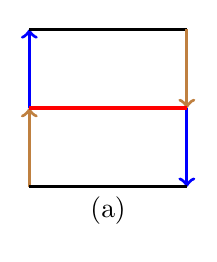
\begin{tikzpicture}
        \draw[color=blue, very thick, ->] (-1,0) -- (-1,1);
        \draw[color=brown, very thick, ->] (-1,-1) -- (-1,0);
        \draw[very thick] (-1,1) -- (1,1);
        \draw[color=brown, very thick, ->] (1,1) -- (1,0);
        \draw[color=blue, very thick, ->] (1,0) -- (1,-1);
        \draw[very thick] (1,-1) -- (-1,-1);
        \draw[color=red, very thick] (-1,0) -- (1,0);
        \node at (0,-1) [below]{(a)};
    \end{tikzpicture}
    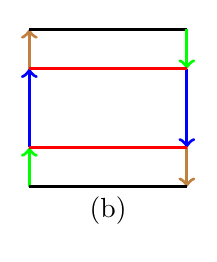
\begin{tikzpicture}
        \draw[color=green, very thick, ->] (-1,-1) -- (-1,-0.5);
        \draw[color=blue, very thick, ->] (-1,-0.5) -- (-1,0.5);
        \draw[color=brown, very thick, ->] (-1,0.5) -- (-1,1);
        \draw[very thick] (-1,1) -- (1,1);
        \draw[color=green, very thick, ->] (1,1) -- (1,0.5);
        \draw[color=blue, very thick, ->] (1,0.5) -- (1,-0.5);
        \draw[color=brown, very thick, ->] (1,-0.5) -- (1,-1);
        \draw[very thick] (1,-1) -- (-1,-1);
        \draw[color=red, very thick] (-1,0.5) -- (1,0.5);
        \draw[color=red, very thick] (-1,-0.5) -- (1,-0.5);
        \node at (0,-1) [below]{(b)};
    \end{tikzpicture}
    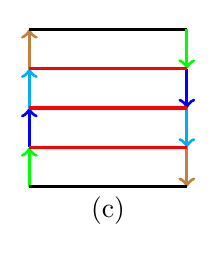
\begin{tikzpicture}
        \draw[color=green, very thick, ->] (-1,-1) -- (-1,-0.5);
        \draw[color=blue, very thick, ->] (-1,-0.5) -- (-1,0);
        \draw[color=cyan, very thick, ->] (-1,0) -- (-1,0.5);
        \draw[color=brown, very thick, ->] (-1,0.5) -- (-1,1);
        \draw[very thick] (-1,1) -- (1,1);
        \draw[color=green, very thick, ->] (1,1) -- (1,0.5);
        \draw[color=blue, very thick, ->] (1,0.5) -- (1,0);
        \draw[color=cyan, very thick, ->] (1,0) -- (1,-0.5);
        \draw[color=brown, very thick, ->] (1,-0.5) -- (1,-1);
        \draw[very thick] (1,-1) -- (-1,-1);
        \draw[color=red, very thick] (-1,0.5) -- (1,0.5);
        \draw[color=red, very thick] (-1,0) -- (1,0);
        \draw[color=red, very thick] (-1,-0.5) -- (1,-0.5);
        \node at (0,-1) [below]{(c)};
    \end{tikzpicture}
    \begin{enumerate}[(a)]
    \item
    如图,由于两次反向粘贴实质为同向,最终结果为圆环。
    
    \item
    如图,边界部分类似(a)知为圆环,中间为M\"obius带,因此结果为一个圆环一个M\"obius带。
    
    \item
    如图,与切割顺序无关,为两个圆环。
    
    \item
    若其中无中间圆,类似(b)可知为$k$个圆环与一个M\"obius带,否则类似(c)可知为$k$个圆环。
    \end{enumerate}
    
    \item
    \begin{enumerate}[(a)]
    \item
    记切割处为$x$,将两个$a$拼接后多边形成为$xxc^{-1}dbcb^{-1}d$,两个$x$可分离为右侧连通和第一个部分,剩余为$c^{-1}dbcb^{-1}d$,再切割出$c^{-1}d$,设切割线为$y$,将两个$d$拼接后多边形成为$yybcb^{-1}c$,两个$x$可分离为右侧连通和第二个部分,剩余$bcb^{-1}c$恰好为第三个部分,从而得证。
    
    \item
    记切割处为$x$,将两个$a$拼接后多边形成为$xbcdx^{-1}c^{-1}d^{-1}b^{-1}$,再切割出$c^{-1}b^{-1}d^{-1}$,设切割线为$y$,将两个$b$拼接后多边形成为$x^{-1}yxyd^{-1}c^{-1}cd$,可分离为$x^{-1}yxy$与$d^{-1}c^{-1}cd$,由讲义Klein瓶的两种多边形表示可知即为对应连通和。
    \end{enumerate}
    
    \item
    \begin{enumerate}[(a)]
    \item
    \begin{enumerate}[(i)]
    \item
    不可能是1个2-单形:否则考虑1-单形上的点,利用习题13.1(4)(b)可知其不存在邻域与平面同胚,矛盾。
    
    不可能是大于等于3个2-单形:否则考虑1-单形上的点的同胚于$\mathbb{R}^2$的邻域,在周边的两个2-单形中各取一个足够小半圆,形成一维紧流形,但去掉此一维紧流形后此邻域仍然连通,与Jordan曲线定理矛盾。
    
    \item
    利用(i),考虑顶点周围的边可知每个顶点周围的2-单形一定可以分为若干个圈,而若超出一个这样的圈,考虑顶点的同胚于$\mathbb{R}^2$的小邻域,在取出顶点后连通分支超过一个,从而矛盾。
    \end{enumerate}
    
    \item
    由其包含于有限个2-单形可知满足A2、T2,从而只需说明局部同胚于$\mathbb{R}^2$开集。
    
    若一点在2-单形上而不在1-单形上,说明其存在邻域只与此2-单形相交,由此局部同胚于平面。
    
    若一点在1-单形上而不在顶点上,取其在两个2-单形中各为半圆的小邻域,从而可同胚于$\mathbb{R}^2$中的开圆。
    
    若一点在顶点上,假设有$n$个2-单形环绕,可类似1-单形情况在每个2-单形中取一段弧相接成圈,此邻域即同胚于$\mathbb{R}^2$中的开集。
    \end{enumerate}
    
    \item
    \begin{enumerate}[(a)]
    \item
    若任何$\sigma_{i_3}$与$P_2$交为至多一点,由连通性考虑其中任意一点处,$P_2$与剩下的2-单形至少排成了两个圈,因此矛盾;若$\sigma_{i_3}\cap P_2$的公共边在$P_2$内部,此条边至少为3个2-单形相交,因此矛盾。从而每次都能取出符合要求相交于边界的$\sigma_i$,即补完了证明。
    
    \item
    考虑多边形划分所对应的三角剖分,边界粘合后满足(3)(b)的条件,因此构成曲面。
    \end{enumerate}
\end{enumerate}

\subsection{}
\begin{enumerate}[(1)]
    \item
    \begin{enumerate}[(a)]
    \item
    $\langle a,b,c,d|acadbcb^{-1}d\rangle\rightsquigarrow\mathbb{RP}^2\#\langle b,c,d|dbcb^{-1}dc^{-1}\rangle\rightsquigarrow\mathbb{RP}^2\#\mathbb{RP}^2\#\langle b,c|c^{-1}bc^{-1}b^{-1}\rangle$
    
    $\rightsquigarrow\mathbb{RP}^2\#\mathbb{RP}^2\#\mathbb{RP}^2\#\mathbb{RP}^2=\widetilde{\Sigma}_4$
    
    \item
    $\langle a,b,c,d,e|abcb^{−1}adede^{−1}\rangle\rightsquigarrow\mathbb{RP}^2\#\langle b,c,d,e|dede^{-1}bcb^{-1}\rangle\rightsquigarrow\mathbb{RP}^2\#\mathbb{RP}^2\#\langle b,c,e|e^{-1}bcb^{-1}e^{-1}\rangle$
    
    $\rightsquigarrow\mathbb{RP}^2\#\mathbb{RP}^2\#\mathbb{RP}^2\#\langle b,c|bcb^{-1}\rangle\rightsquigarrow\mathbb{RP}^2\#\mathbb{RP}^2\#\mathbb{RP}^2\#D=\widetilde{\Sigma}_{3,1}$
    
    \item
    将中间的交叉处上下交换后利用几何形变可知其为$\Sigma_{1,1}$。
    
    \item
    “过街天桥”与“地下通道”的交换不影响曲面的同胚,先不考虑右上角的$\#\mathrm{T}^2$,可发现交换后剩下部分为$\Sigma_{1,1}$,故最终结果为$\Sigma_{2,1}$。
    \end{enumerate}
    
    \item
    \begin{enumerate}[(a)]
    \item
    1:考虑其任何一个三角剖分的定向,由于三角剖分的性质,类似证明多边形表示的存在性,通过边界相接可以将一个三角形上的定向扩展到每个三角形上,因此反转任何三角形的定向都会反转所有三角形的定向,而此恰为与反转前相反的定向,从而对给定定向存在唯一一个与它不同的定向,即得证。
    
    2:利用连通和的良定性可不妨假设分别在$M_1,M_2$三角剖分的某个三角形三边各取一点,从中挖去小三角形,此时剩下三个三角形的边界由原三角形的边界有定向,再将两个小三角形对应边按相同定向粘贴,则剪开的两个三角形在粘贴后成为六个三角形,且保持定向、与其他部分无关,从而$M_1\#M_2$可定向。
    
    3:利用加细可考虑有一部分三角形能同胚于M\"obius带的三角剖分,若此三角剖分存在定向,则去除此部分外的三角形后保持定向,从而M\"obius带可定向,矛盾。
    
    \item
    对$S^2$,可不妨设其为$\max(|x|,|y|,|z|)=1$的立方体,由此$f(x,y,z)=(x,y,-z)$即构成反转定向的同胚,下面就$k$与$m$增加时归纳,使$f$仍为反转定向的同胚:
    
    在$k$增加时,在$x=-1$的一侧可任意增添$1\times1\times1$但中间被竖直挖去的立方体并将相交的面移出,在$m$增加时可在$x=1$的面上挖去沿$z$轴对称的小正方形,由此两操作独立可知任何$\Sigma_{k,m}$可通过有限操作得到,而由于$z=1,y=1,z=-1$的面没有改变,考虑这三个面的三角剖分可知操作后$f$仍为反转定向的同胚,从而得证。
    \end{enumerate}
    
    \item
    \begin{enumerate}[(a)]
    \item
    $\chi(S^2)=2\chi(\mathbb{RP}^2)=2,\chi(\Sigma_{11})=5\chi(\Sigma_3)=-20$
    
    \item
    $\chi(S_1)=k\chi(S_2)$
    
    证明:由紧性,考虑每点处邻域可取三角剖分使得每一个三角形$K$的内部既在某点的局部欧氏邻域中,又在满足覆叠性质的邻域中。此时,$p^{-1}(K)$同胚于$k$个三角形,且由覆叠映射性质可知不同三角形对应的$p^{-1}(K)$内部不交,利用Jordan-Schoenflies定理可将所有$p^{-1}(K)$的边界调整为所需的三角形,从而可从边界构造三角剖分,此时顶点的提升仍然为顶点,边的提升仍然为边,面的提升仍然为面,因此$|V|,|E|,|F|$均成为对应的$k$倍,从而由欧拉示性数定义得证。
    
    \item
    当$n-1|m-1$时,类似构造$\Sigma_{11}$到$\Sigma_3$覆叠可构造覆叠,而不满足此条件时由(b)可知不存在覆叠,从而此即为充要条件。
    
    \item
    先考虑$\widetilde{\Sigma}_l$,其覆叠一定为无边紧连通曲面,又由条件可定向考虑欧拉示性数知为$\Sigma_{l-1}$,而在其挖去$m$个圆盘后,利用分离性可知二重覆叠空间中将挖去$2m$个圆盘,因此$\Sigma_{l-1,2m}$为$\widetilde{\Sigma}_{l,m}$的二重覆叠。
    \end{enumerate}
    
    \item
    \begin{enumerate}[(a)]
    \item
    由每条边周围有两个面,每个面有三条边可知结论成立。
    
    \item
    由$\chi(S)=|V|-|E|+|F|$与(a)即有结论。
    
    \item
    由边数不超过任何两点连线可知$|E|\le\frac{|V|(|V|-1)}{2}$,代入(b)化简得$|V|^2-7|V|+6\chi(S)\ge0$,由于二次方程另一解导致$|V|$不超过3,不可能,因此结论成立。
    \end{enumerate}
\end{enumerate}
\end{document}